\documentclass[10pt,conference]{IEEEtran}
\usepackage{cite}
\usepackage{amsmath,amssymb,amsfonts}
\usepackage{algorithmic}
\usepackage{graphicx}
\usepackage{textcomp}
\usepackage{xcolor}
\usepackage{tikz}
\usepackage[hyphens]{url}
\usepackage{fancyhdr}
\usepackage{hyperref}
\usepackage{booktabs}
\usepackage{array}
\usepackage{enumitem}
\usepackage{xcolor}
\usepackage{hyperref}
\usepackage{graphicx}
\usepackage{caption}
\usepackage{subcaption}
\usepackage{multirow}
\usepackage{svg}
\usepackage{float}
\usepackage{placeins}
\usepackage[table]{xcolor}
\usepackage{tabularx}
\usepackage{kotex}
\usepackage{svg} 
\usepackage{comment}
\newcolumntype{Y}{>{\centering\arraybackslash}X}

% Ensure letter paper
\pdfpagewidth=8.5in
\pdfpageheight=11in

\newcommand{\hpcayear}{2027}
\newcommand{\todo}[1]{\textcolor{red}{[TODO: #1]}}
\newcommand{\ours}{\textsc{FINISH}}
\newcommand{\fpint}{FP-INT}
\newcommand{\wkv}{WKV}
\newcommand{\tc}{Tensor Core}
\newcommand{\mxu}{MXU}
\newcommand{\qcol}{Q-COL}
\newcommand{\qrow}{Q-ROW}
\newcommand{\Cone}{FP TCU Baseline}
\newcommand{\Ctwo}{Linear Only FP-INT}
\newcommand{\Cthr}{Naive WKV FP-INT}
\newcommand{\Cfou}{FINISH}
\newcommand{\blackcircletext}[1]{%
  \tikz[baseline=-0.5ex]{
    \node[
      circle,
      fill=black,
      text=white,
      inner sep=0pt,
      minimum size=7pt,
      font=\fontsize{5}{5}\selectfont\bfseries
    ] (char) {#1};
  }%
}

\setlength{\abovedisplayskip}{3pt}
\setlength{\belowdisplayskip}{3pt}
\setlength{\abovedisplayshortskip}{2pt}
\setlength{\belowdisplayshortskip}{2pt}


%%%%%%%%%%%%%%%%%%%%%%%%%%%%%%%%%%%%%%%%
%%%%%%%%%%%%%% -- UPDATE -- %%%%%%%%%%%%%%%
\newcommand{\hpcasubmissionnumber}{NaN}
\title{FINISH: An End-to-End FP–INT LLM Inference System with Quantized Weights and KV Cache}
%%%%%%%%%%%%%%%%%%%%%%%%%%%%%%%%%%%%%%%%


%%%%%%%%%%%%%%%%%%%%%%%%%%%%%%%%%%%%%%%%
%%%%%%%% -- ONLY FOR CAMERA READY -- %%%%%%%%
%\def\hpcacameraready{} % Uncomment to build camera-ready version
\newcommand{\hpcapubid}{0000--0000/00\$00.00}
\newcommand\hpcaauthors{First Author$\dagger$ and Second Author$\ddagger$}
\newcommand\hpcaaffiliation{First Affiliation$\dagger$, Second Affiliation$\ddagger$}
\newcommand\hpcaemail{Email(s)}

%%%%% -- ARTEFACT EVALUATION RESULTS -- %%%%%%
% Uncomment the following based on the badges that were awarded to this paper
%\def\aeopen{}           % The artifact is publically available
%\def\aereviewed{}     % The artefact has been reviewed
%\def\aereproduced{} % The results have been reproduced
%%%%%%%%%%%%%%%%%%%%%%%%%%%%%%%%%%%%%%%%

%%%%%%%%%%%%%%%%%%%%%%%%%%%%%%%%%%%%%
%%%%%%%%%% -- DO NOT MODIFY -- %%%%%%%%%%
%%%%%%%%%%%%%%%%%%%%%%%%%%%%%%%%%%%%%

\author{
  \ifdefined\hpcacameraready
    \IEEEauthorblockN{\hpcaauthors{}}
      \IEEEauthorblockA{
        \hpcaaffiliation{} \\
        \hpcaemail{}
      }
  \else
    \IEEEauthorblockN{\normalsize{HPCA \hpcayear{} Submission
      \textbf{\#\hpcasubmissionnumber{}}} \\
      \IEEEauthorblockA{
        Confidential Draft \\
        Do NOT Distribute!!
      }
    }
  \fi 
}

% Heading and footer for title page
\fancypagestyle{camerareadyfirstpage}{%
  \fancyhead{}
  \renewcommand{\headrulewidth}{0pt}
  \fancyhead[C]{
    \ifdefined\aeopen
    \parbox[][12mm][t]{13.5cm}{\hpcayear{} IEEE International Symposium on High-Performance Computer Architecture (HPCA)}    
    \else
      \ifdefined\aereviewed
      \parbox[][12mm][t]{13.5cm}{\hpcayear{} IEEE International Symposium on High-Performance Computer Architecture (HPCA)}
      \else
      \ifdefined\aereproduced
      \parbox[][12mm][t]{13.5cm}{\hpcayear{} IEEE International Symposium on High-Performance Computer Architecture (HPCA)}
      \else
      \parbox[][0mm][t]{13.5cm}{\hpcayear{} IEEE International Symposium on High-Performance Computer Architecture (HPCA)}
    \fi 
    \fi 
    \fi 
    \ifdefined\aeopen 
      \includegraphics[width=12mm,height=12mm]{ae-badges/open-research-objects.pdf}
    \fi 
    \ifdefined\aereviewed
      \includegraphics[width=12mm,height=12mm]{ae-badges/research-objects-reviewed.pdf}
    \fi 
    \ifdefined\aereproduced
      \includegraphics[width=12mm,height=12mm]{ae-badges/results-reproduced.pdf}
    \fi
  }
  %\fancyfoot[L]{\hpcapubid{} \copyright \hpcayear{} IEEE}
  \fancyfoot[C]{}
}
% Heading and footer for remaining pages
\fancyhead{}
\renewcommand{\headrulewidth}{0pt}
%\fancyhead[C]{\hpcayear{} IEEE International Symposium on
% High-Performance Computer Architecture (HPCA)}


\begin{document}
\maketitle

%Enables the camera ready header and footer
\ifdefined\hpcacameraready 
  \thispagestyle{camerareadyfirstpage}
  \pagestyle{empty}
\else
  \thispagestyle{plain}
  \pagestyle{plain}
\fi

\newcommand{\hpcaheight}{0mm}
\ifdefined\eaopen
\renewcommand{\hpcaheight}{12mm}
\fi
  


%%%%%%%%%%%%%%%%%%%%%%%%%%%%%%%%%%%%%%%%
%%%%%%%% -- PAPER CONTENT STARTS -- %%%%%%%%%

\begin{abstract}
LLM inference is increasingly deployed with both weight and KV cache quantization. In such weight and KV cache (WKV) quantized models, the core GEMMs operate on FP activations and INT weights or KV tensors. Today's GPUs execute this pattern by dequantizing INT operands on the fly and running the resulting FP$\times$FP product on Tensor Cores. This reduces memory traffic, but loses the compute- and energy-side benefits of quantization. Prior \fpint{} hardware also falls short because it mainly targets linear layers and leaves long-context attention on the conventional FP path.

This paper presents \ours{}, a hardware/software system that turns array-level \fpint{} efficiency into system-level LLM speedup. First, we propose a matrix multiplication unit (MXU) and an \fpint{} attention kernel that together support multiple KV quantization directions, so both linear layers and quantized KV attention execute on the same \fpint{} datapath.
%Second, we co-design a decoupled GEMM engine, high-bandwidth tensor memory and direct-connected memory path to keep the larger array utilized.
Second, we co-design a decoupled GEMM engine and a high-bandwidth tensor-memory subsystem with a low-cost, restricted tensor interconnect to sustain high utilization of the enlarged array.
Third, we extend the open-source Vortex GPGPU into an end-to-end stack and evaluate four design points to quantify how much unit-level efficiency each architectural step delivers at the system level. On a real FPGA prototype, \ours{} reduces area-normalized end-to-end latency over the FP Tensor Core baseline by 3.24$\times$ in prefill and 4.73$\times$ in decode on geomean (up to 4.31$\times$ and 7.96$\times$), and energy per token by 4.75$\times$ and 7.93$\times$.

\end{abstract}

\section{Introduction}

% \paragraph{The shift in LLM quantization.}
% Weight quantization is already widely deployed in LLM inference. Weight-only quantization keeps activations in FP and stores weights in INT4/INT8 to reduce model footprint and memory traffic. Activations and queries are input-dependent and dynamic, which makes aggressive quantization difficult, but weights can be quantized offline with a variety of techniques that minimize the resulting error~\cite{frantar2022gptq,lin2023awq,dettmers2023spqr,kim2023squeezellm,lee2023owq,kim2023finequant,shao2023omniquant,chee2023quip,tseng2024quipsharp,shang2023pbllm,egiazarian2024aqlm,huang2024billm,malinovskii2024pvtuning,tseng2024qtip,liu2024vptq,luo2024daq,lee2024lrq,yan2026d2quant,xu2025butterflyquant,liu2024spinquant}. Reducing weights to a low bit width directly reduces memory-traffic latency, and the saved capacity can also be spent on a larger model or a longer KV cache to improve accuracy.

% As modern LLMs scale to long-context and high-throughput serving, however, the KV cache itself has become a new memory bottleneck. At context lengths beyond 32k or 128k, the KV cache can demand memory capacity and bandwidth comparable to the model weights. LLM inference has therefore moved beyond weight-only quantization toward \wkv{} quantization, in which both the weights and the KV cache are quantized.
Large language models (LLMs) have become core AI workloads, but increasing model sizes and context lengths make inference increasingly constrained by memory capacity, memory bandwidth, and compute cost. Efficient serving must therefore reduce both data movement and arithmetic overhead rather than optimizing either in isolation.

Quantization is one of the most effective techniques for reducing inference cost. Weight-only quantization keeps activations in FP while storing weights in INT4 or INT8, reducing model footprint and per-token weight traffic~\cite{frantar2022gptq,lin2023awq,dettmers2023spqr,kim2023squeezellm,lee2023owq,kim2023finequant,shao2023omniquant,chee2023quip,tseng2024quipsharp,shang2023pbllm,egiazarian2024aqlm,huang2024billm,malinovskii2024pvtuning,tseng2024qtip,liu2024vptq,luo2024daq,lee2024lrq,yan2026d2quant,xu2025butterflyquant,liu2024spinquant}. The saved capacity can be used for a larger model, a longer context, or a larger serving batch, improving the accuracy--throughput--cost tradeoff.

As LLM serving moves toward long contexts and high throughput, however, the KV cache becomes another major source of capacity and bandwidth pressure. Attention computation also grows with the attended sequence length and becomes a substantial fraction of prefill latency at long contexts, as shown in Figure~\ref{fig:long_seq_atten_overhead}. Recent methods therefore quantize both model weights and the KV cache~\cite{yue2024wkvquant,liu2024spinquant}. We refer to this approach as weight-and-KV-cache (\wkv{}) quantization.

This shift changes the arithmetic form of the dominant GEMMs as well as the memory traffic. In a \wkv{}-quantized model, linear and FFN layers multiply FP activations by INT weights. Quantized attention follows the same pattern: $QK^T$ multiplies FP queries by INT keys, while $PV$ multiplies FP probabilities by INT values~\cite{figna,yue2024wkvquant,liu2024spinquant}. Realizing the full benefit of \wkv{} quantization therefore requires efficient \fpint{} execution across both linear and attention layers.

Existing GPUs execute these operations by dequantizing the INT operand and then using an FP$\times$FP Tensor Core. Software kernels such as Marlin~\cite{marlin} and BitDecoding~\cite{bitdecoding} can fuse and hide much of the dequantization latency, but every MAC still executes on the FP$\times$FP datapath. They therefore capture the memory benefit of quantization without exploiting the higher compute density and energy efficiency available from a native \fpint{} unit. This limitation becomes increasingly important as MQA, GQA, MLA, batching, and quantization raise arithmetic intensity~\cite{mqa,gqa,deepseekai2024deepseekv2strongeconomicalefficient}.

Prior hardware studies, including FIGNA, FIGLUT, ANDA, and LUT Tensor Core~\cite{figna,figlut,anda,lut_tensor_core}, improve array-level TOPS/mm$^2$ and TOPS/W using specialized \fpint{} datapaths. However, two system-level limitations remain. First, most designs accelerate linear-layer GEMMs but leave quantized KV attention on the conventional FP path, and existing attention-oriented designs cannot efficiently handle various quantization methods. Second, increasing \fpint{} array density also raises operand- and partial-sum-bandwidth demand. Scaling conventional register-file, cache, local-memory, DMA, and crossbar structures with the array can erode the area and energy advantages of the denser \fpint{} datapath.

This paper presents \ours{}, an end-to-end hardware/software system that translates native \fpint{} array efficiency into LLM-inference performance. \ours{} integrates a quantization-direction-reconfigurable \fpint{} GEMM engine that supports both linear and quantized-attention GEMMs, a partitioned tensor-memory subsystem with fixed interleaved connectivity and specialized DMA engines, and layout/runtime support that satisfies the resulting alignment and bank-mapping constraints. The GEMM engine remains decoupled from the SIMT pipeline, which executes control-intensive and vector operations, while a dedicated tensor path supplies the larger MXU without proportionally scaling the general-purpose memory fabric.

Our key contributions can be summarized as follows:
\begin{itemize}[leftmargin=*]
    \item \textbf{Native \fpint{} execution for linear and quantized-attention GEMMs.} We propose a quantization-direction-reconfigurable GEMM engine that supports both \qcol{} and \qrow{} execution and independently configures standard or transposed loading of the INT operand. The same physical MXU therefore executes linear layers, $QK^T$, and $PV$ without falling back to an FP Tensor Core in either prefill or decode.

    \item \textbf{A tensor-memory system that sustains a denser \fpint{} MXU.} We decouple the GEMM engine from the SIMT datapath and partition on-chip storage into general-purpose local memory, dedicated tensor memory, and accumulator memory. Fixed one-to-one or interleaved connectivity, together with specialized T-DMA and G-DMA engines, supplies tensor operands without proportionally scaling the general-purpose crossbar and cache paths.

    \item \textbf{Constraint-aware layout and runtime support.} We use tile-major tensor layouts, alignment-aware allocation, and fused layout transformation to satisfy the address-alignment and bank-mapping constraints introduced by the simplified tensor path while avoiding a standalone transformation pass.

    \item \textbf{An end-to-end system implementation and evaluation on an FPGA platform.} We implement \ours{} by extending the Vortex GPGPU, including its hardware, runtime, and native LLM kernels, and evaluate four incremental design points to isolate how each component converts array-level efficiency into system-level performance. The FPGA prototype with HBM achieves up to $4.31\times$ lower area-normalized prefill latency and up to $7.96\times$ lower area-normalized decode latency than the FP Tensor Core baseline.
\end{itemize}

%%%%%%%%%%%%%%%%%%%%%%%\iffalse
\begin{comment}
Large language models (LLMs) have become core AI workloads, but growing model sizes and context lengths have made inference cost a first-order systems problem. Memory capacity, memory bandwidth, and compute demand all scale with every token, so efficient serving must reduce both data movement and arithmetic cost.
 
Quantization is one of the most effective solutions. Weight-only quantization keeps activations in FP while storing weights in INT4 or INT8, shrinking both model footprint and per-token weight bandwidth~\cite{frantar2022gptq,lin2023awq,dettmers2023spqr,kim2023squeezellm,lee2023owq,kim2023finequant,shao2023omniquant,chee2023quip,tseng2024quipsharp,shang2023pbllm,egiazarian2024aqlm,huang2024billm,malinovskii2024pvtuning,tseng2024qtip,liu2024vptq,luo2024daq,lee2024lrq,yan2026d2quant,xu2025butterflyquant,liu2024spinquant}.\todo{reference check하자} The saved capacity can be spent on a larger model, a longer KV cache, or a larger serving batch, improving the accuracy-throughput-cost tradeoff.
 
As LLMs scale toward long-context and high-throughput serving, the KV cache creates growing capacity and bandwidth pressure. The attention GEMMs also grow with the attended sequence length and become a substantial fraction of prefill computation at long contexts, as shown in Figure~\ref{fig:long_seq_atten_overhead}. Recent methods therefore quantize both weights and the KV cache~\cite{yue2024wkvquant,liu2024spinquant}. We refer to this approach as weight and KV cache (\wkv{}) quantization. This shift reduces memory traffic, but it also changes the core arithmetic pattern and exposes a mismatch with today's accelerators.

\textbf{Key observation: WKV quantization turns the core GEMMs into FP-INT operations.}
In a \wkv{} quantized model, the linear layers multiply an FP activation matrix by an INT weight matrix. 
In attention, $QK^T$ multiplies the FP $Q$ matrix by the INT $K$ matrix, and $PV$ multiplies the FP attention-score matrix $P$ by the INT $V$ matrix~\cite{figna,yue2024wkvquant,liu2024spinquant}.
% , $QK^T$ multiplies FP queries by INT keys, and PV multiplies FP probabilities by INT values~\cite{figna,yue2024wkvquant,liu2024spinquant}. Each core GEMM therefore has one FP operand and one INT operand. Turning \wkv{} quantization into performance requires executing these \fpint{} GEMMs efficiently.

\textbf{Problem: memory saving alone is not enough.}
On-the-fly dequantization lets existing FP$\times$FP Tensor Cores run these kernels, but it forfeits quantization's compute-side benefit.
As attention variants such as MQA, GQA, and MLA reduce per-token KV traffic, and high-batch serving and speculative decoding raise compute demand, compute-path efficiency becomes the limiter~\cite{specdec, mqa, gqa, deepseekai2024deepseekv2strongeconomicalefficient}.
% As MQA/GQA/MLA and high-batch serving raise arithmetic intensity, compute-path efficiency becomes the limiter.

\textbf{Limits of prior software optimization.}
Software \fpint{} GEMM kernels such as Marlin~\cite{marlin} and BitDecoding~\cite{bitdecoding} hide much of the dequantization latency, but existing Tensor Cores cannot multiply FP activations by INT weights directly. These kernels must still convert the INT weights to FP and execute every MAC on the FP$\times$FP datapath, so they cannot exploit the much higher compute-energy efficiency of a native \fpint{} unit.

\textbf{Limits of prior hardware research.}
FIGNA, FIGLUT, ANDA, and LUT Tensor Core~\cite{figna, figlut, anda, lut_tensor_core} improve array-level TOPS/mm$^2$ and TOPS/W with \fpint{} units, but two system gaps remain. First, most designs accelerate only linear layers and leave quantized KV attention on the FP path. Second, larger \fpint{} arrays require proportional register, memory, DMA, and interconnect bandwidth, so array density does not automatically become system-level speedup.

\textbf{Goal and approach of this paper.}
We co-design the GEMM engine, memory subsystem, and kernel/runtime stack so \fpint{} array efficiency translates into end-to-end LLM performance.
%\ours{} accelerates both linear and attention GEMMs with a transposable GEMM unit that supports multiple KV quantization directions.
\ours{} accelerates both linear and attention GEMMs with a RHS-axis-reconfigurable GEMM engine that supports multiple KV quantization directions.
It decouples the GEMM engine from the SIMT lanes and feeds it through a low-cost, restricted tensor interconnect. The runtime and kernels then satisfy the resulting address constraints through layout, allocation, and fusion.

\textbf{Contributions.}
This paper makes the following contributions.
\begin{itemize}[leftmargin=*]
    \item \textbf{Native \fpint{} attention execution at both prefill and decode.}
    We propose a GEMM engine and kernels that execute both linear layers and quantized KV attention as native \fpint{} GEMMs, improving both TTFT and TPOT.

    \item \textbf{Decoupled GEMM engine and low-cost tensor interconnect.}
    We decouple the GEMM engine from SIMT and feed it with split local/tensor memory, a restricted high-bandwidth tensor interconnect, and cache-bypass DMA.

    \item \textbf{Layout-optimization kernels and runtime extensions.}
    We resolve modulo-based address constraints with layout optimization, fusion, and memory-allocation-aware runtime support.

    % \item \textbf{E2E \fpint{} accelerator implementation and system evaluation.}
    \item \textbf{End-to-End WKV inference system and incremental system-level evaluation.}
    We implement the proposed \fpint{} compute and memory architecture as a complete accelerator system that includes an FPGA prototype and the runtime support and native kernels required to execute LLM workloads. We reuse and extend the existing Vortex software infrastructure and incrementally compare four design points to isolate which components convert array level gains into system level speedup. On real hardware, \Cfou{} achieves up to $4.31\times$ lower area-normalized prefill latency and up to $7.96\times$ lower area-normalized decode latency than the FP Tensor Core baseline.
\end{itemize}
\end{comment}
%%%%%%%%%%%%%%%%%\fi

\section{Background and Motivation}
\subsection{WKV-Quantized LLM Inference}

The main operations of LLM inference are the Q/K/V linear projections, attention-score computation ($QK^T$), attention-value product ($PV$), output projection, and FFN layers. Under weight-only quantization, the linear and FFN layers become products between FP activations and INT weights. When KV-cache quantization is also applied, the K and V tensors are stored in INT, so both attention GEMMs likewise become \fpint{} operations: $QK^T$ multiplies an FP Q tensor by an INT K tensor, while $PV$ multiplies an FP probability tensor by an INT V tensor.

Letting $S_*$ and $Z_*$ denote quantization scales and zero points, respectively, the principal kernels of \wkv{}-quantized inference can be summarized as
\begin{align}
    Y_{\mathrm{linear},fp}
    &=
    X_{fp}
    \left(
        \left(
            W_{int}
            -
            Z_W
        \right)
        \odot
        S_W
    \right),
    \\
    P_{fp}
    &=
    \mathrm{softmax}
    \left(
        \frac{
            Q_{fp}
            \left(
                \left(
                    K_{int}
                    -
                    Z_K
                \right)
                \odot
                S_K
            \right)^T
        }{
            \sqrt{d_k}
        }
    \right),
    \\
    O_{fp}
    &=
    P_{fp}
    \left(
        \left(
            V_{int}
            -
            Z_V
        \right)
        \odot
        S_V
    \right).
\end{align}

Figure~\ref{fig:fpint_inference} contrasts three execution paths. A conventional GPU dequantizes the INT weight and KV operands before executing FP$\times$FP GEMMs. Prior \fpint{} accelerators improve linear-layer execution but leave quantized attention on the FP path. In this work, we aim at building the execution path which consumes INT operands natively in both linear layers and the $QK^T$ and $PV$ attention kernels.

\begin{figure}[t]
    \centering
    \begin{subfigure}[t]{\linewidth}
        \centering
        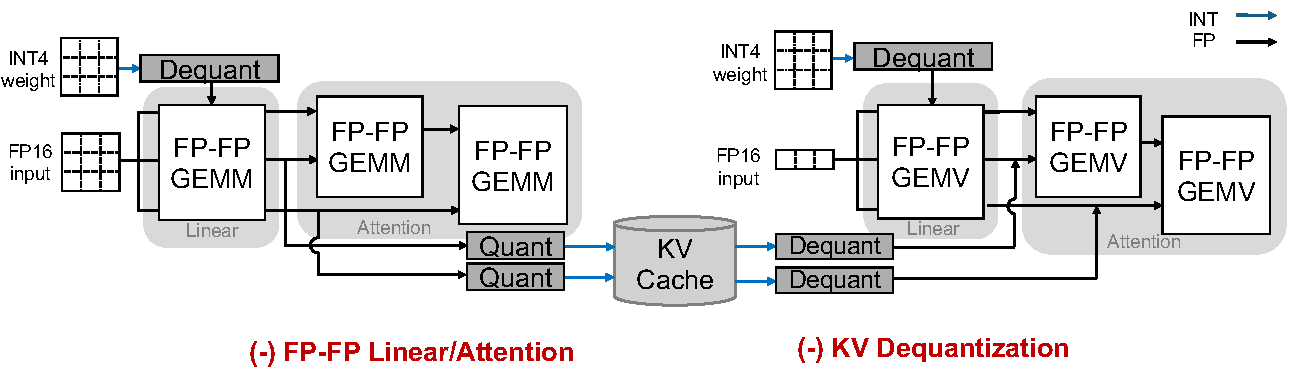
\includegraphics[width=0.95\linewidth]{figures/fig1_a.pdf}
        \caption{A conventional GPU dequantizes INT weight and KV operands before FP GEMM.}
        \label{fig:conventional-gpu}
    \end{subfigure}
    \vspace{0.5em}
    \begin{subfigure}[t]{\linewidth}
        \centering
        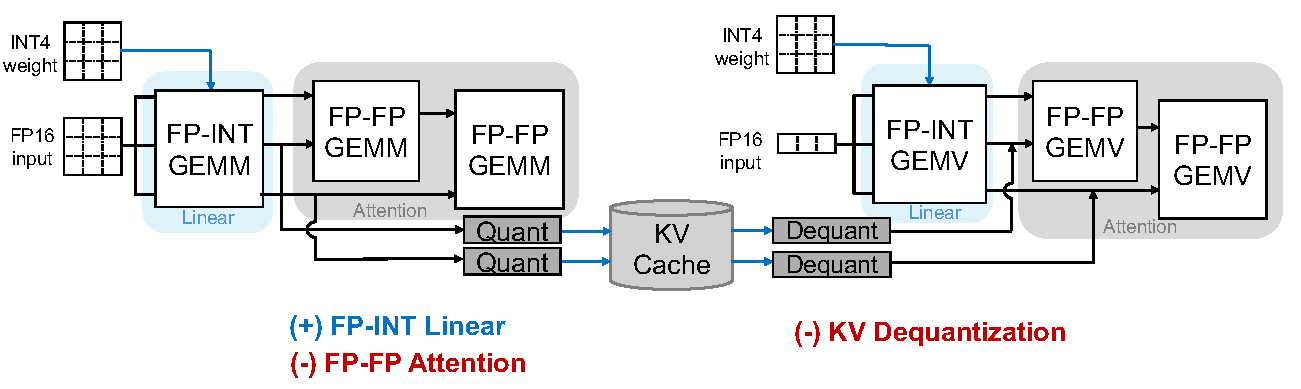
\includegraphics[width=0.95\linewidth]{figures/fig1_b.pdf}
        \caption{Prior \fpint{} accelerators support linear layers but leave attention on the FP path.}
        \label{fig:prior-fpint}
    \end{subfigure}
    \vspace{0.5em}
    \begin{subfigure}[t]{\linewidth}
        \centering
        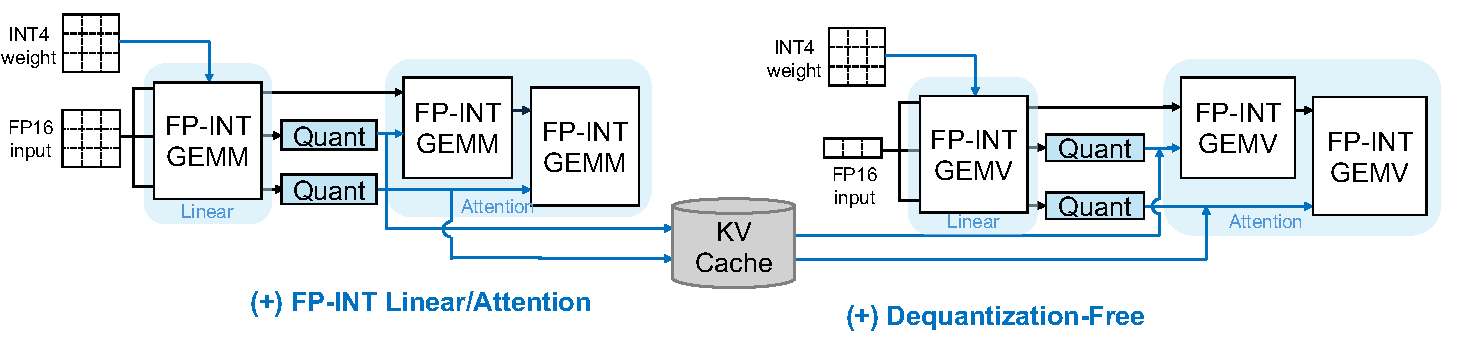
\includegraphics[width=0.99\linewidth]{figures/fig1_c.pdf}
        \caption{The proposed design executes both linear and attention GEMMs using native \fpint{} datapaths.}
        \label{fig:target-fpint}
    \end{subfigure}
    \caption{Execution paths for \wkv{}-quantized inference.}
    \label{fig:fpint_inference}
\end{figure}

\subsection{Why Memory Savings Alone Are Insufficient}

Quantization first reduces memory footprint and traffic, but it does not eliminate compute pressure. Prefill processes the prompt in parallel and is generally compute-bound. Decode is often memory-bound because it proceeds token by token and repeatedly reads the KV cache, but GQA, MQA, MLA, batching, and quantization increase arithmetic intensity and can move decode closer to the compute-bound regime. As illustrated in Figure~\ref{fig:bottleneck-analysis}, modern LLM serving therefore needs a datapath that processes quantized operands directly rather than reducing memory traffic only to dequantize them onto an FP unit.

\begin{figure}[t]
    \centering
    \begin{subfigure}[t]{\linewidth}
        \centering
        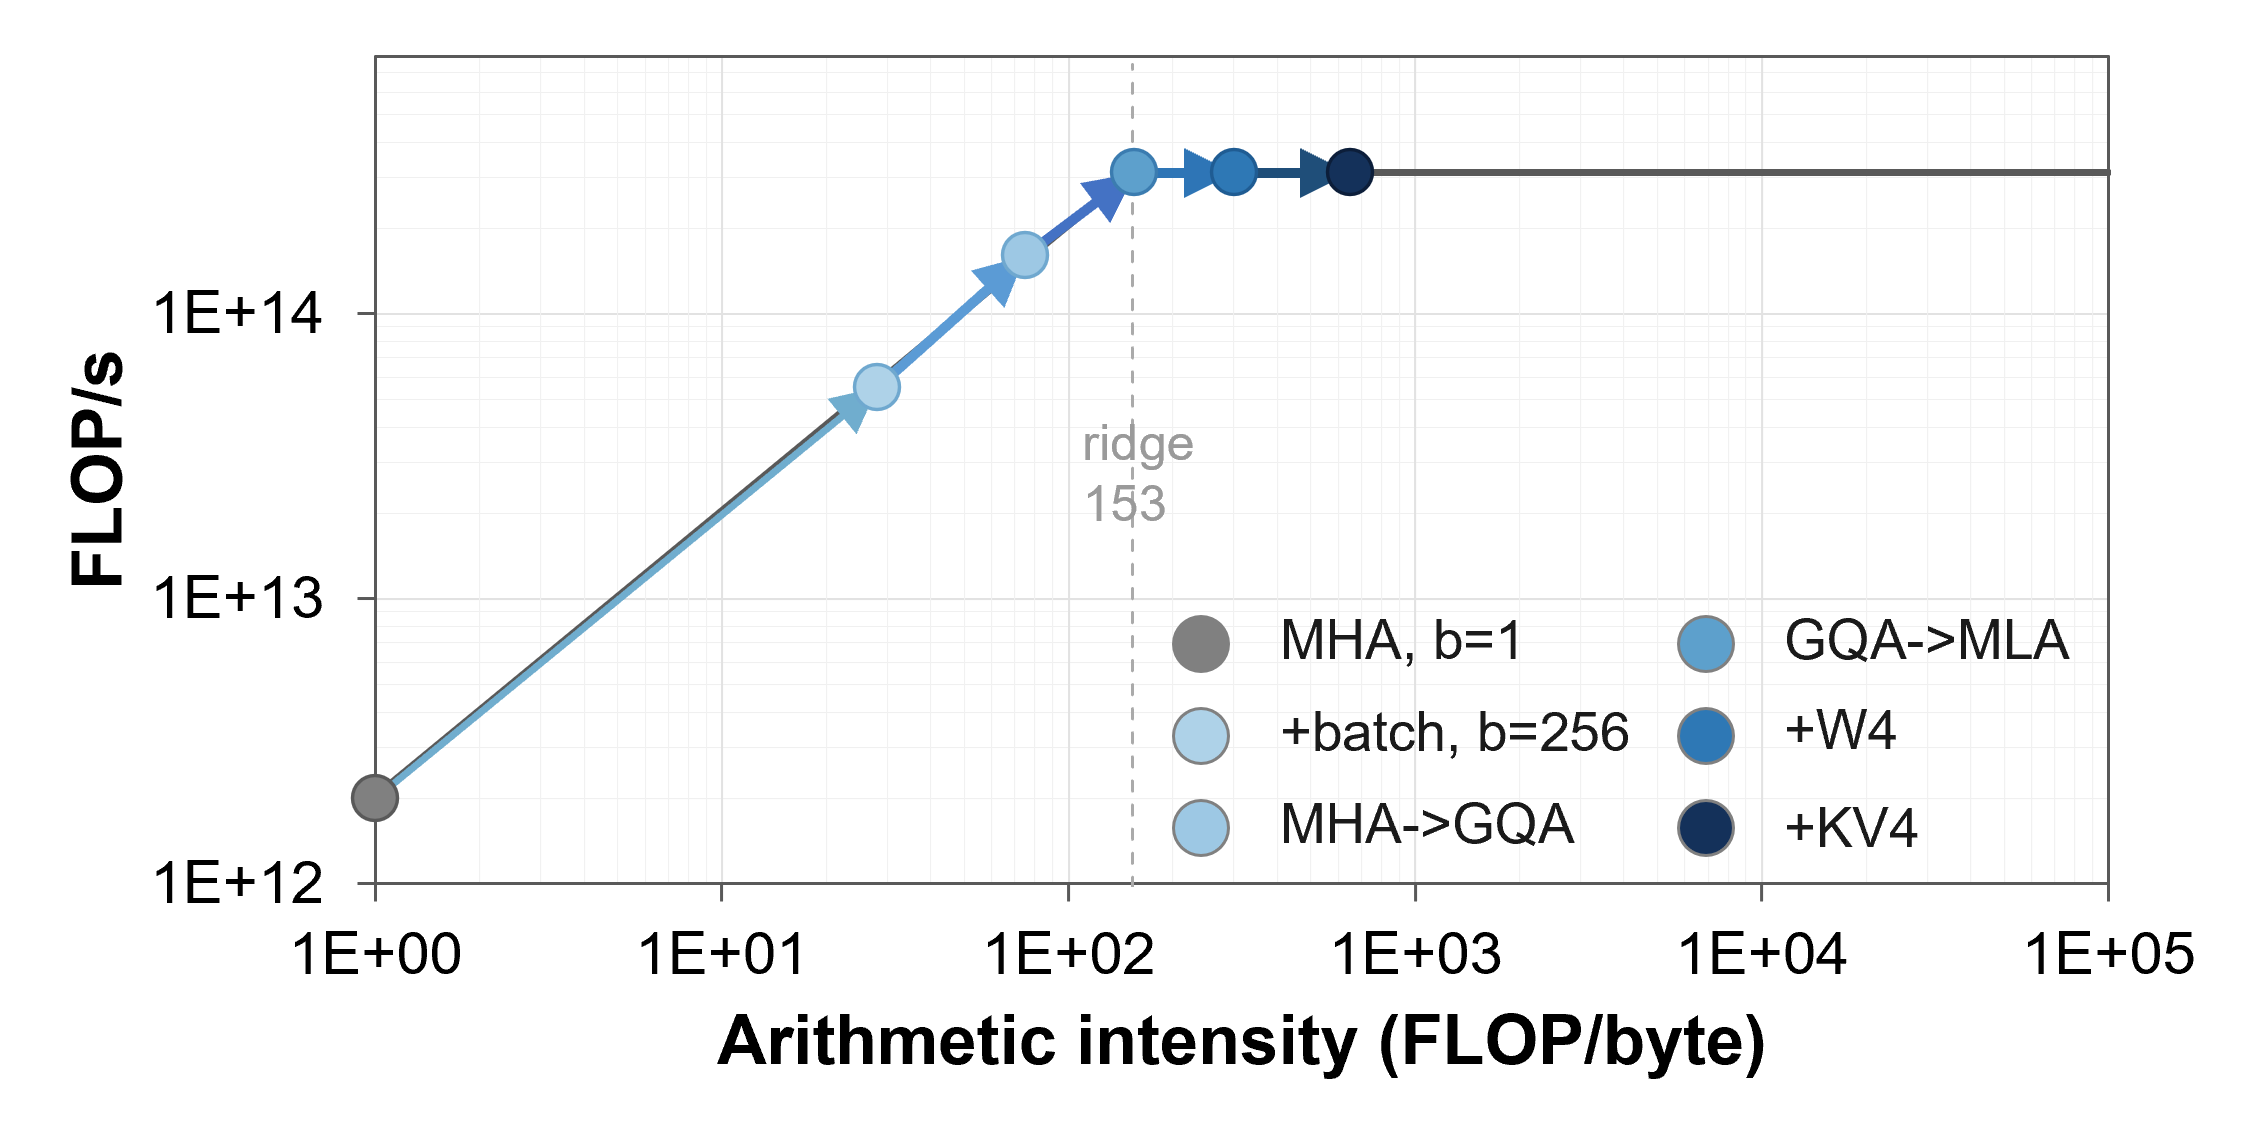
\includegraphics[width=0.92\linewidth]{figures/roofline_decode.png}
        \caption{Decode with a sequence length of 1024.}
        \label{fig:roofline_decode}
    \end{subfigure}
    \vspace{0.5em}
    \begin{subfigure}[t]{\linewidth}
        \centering
        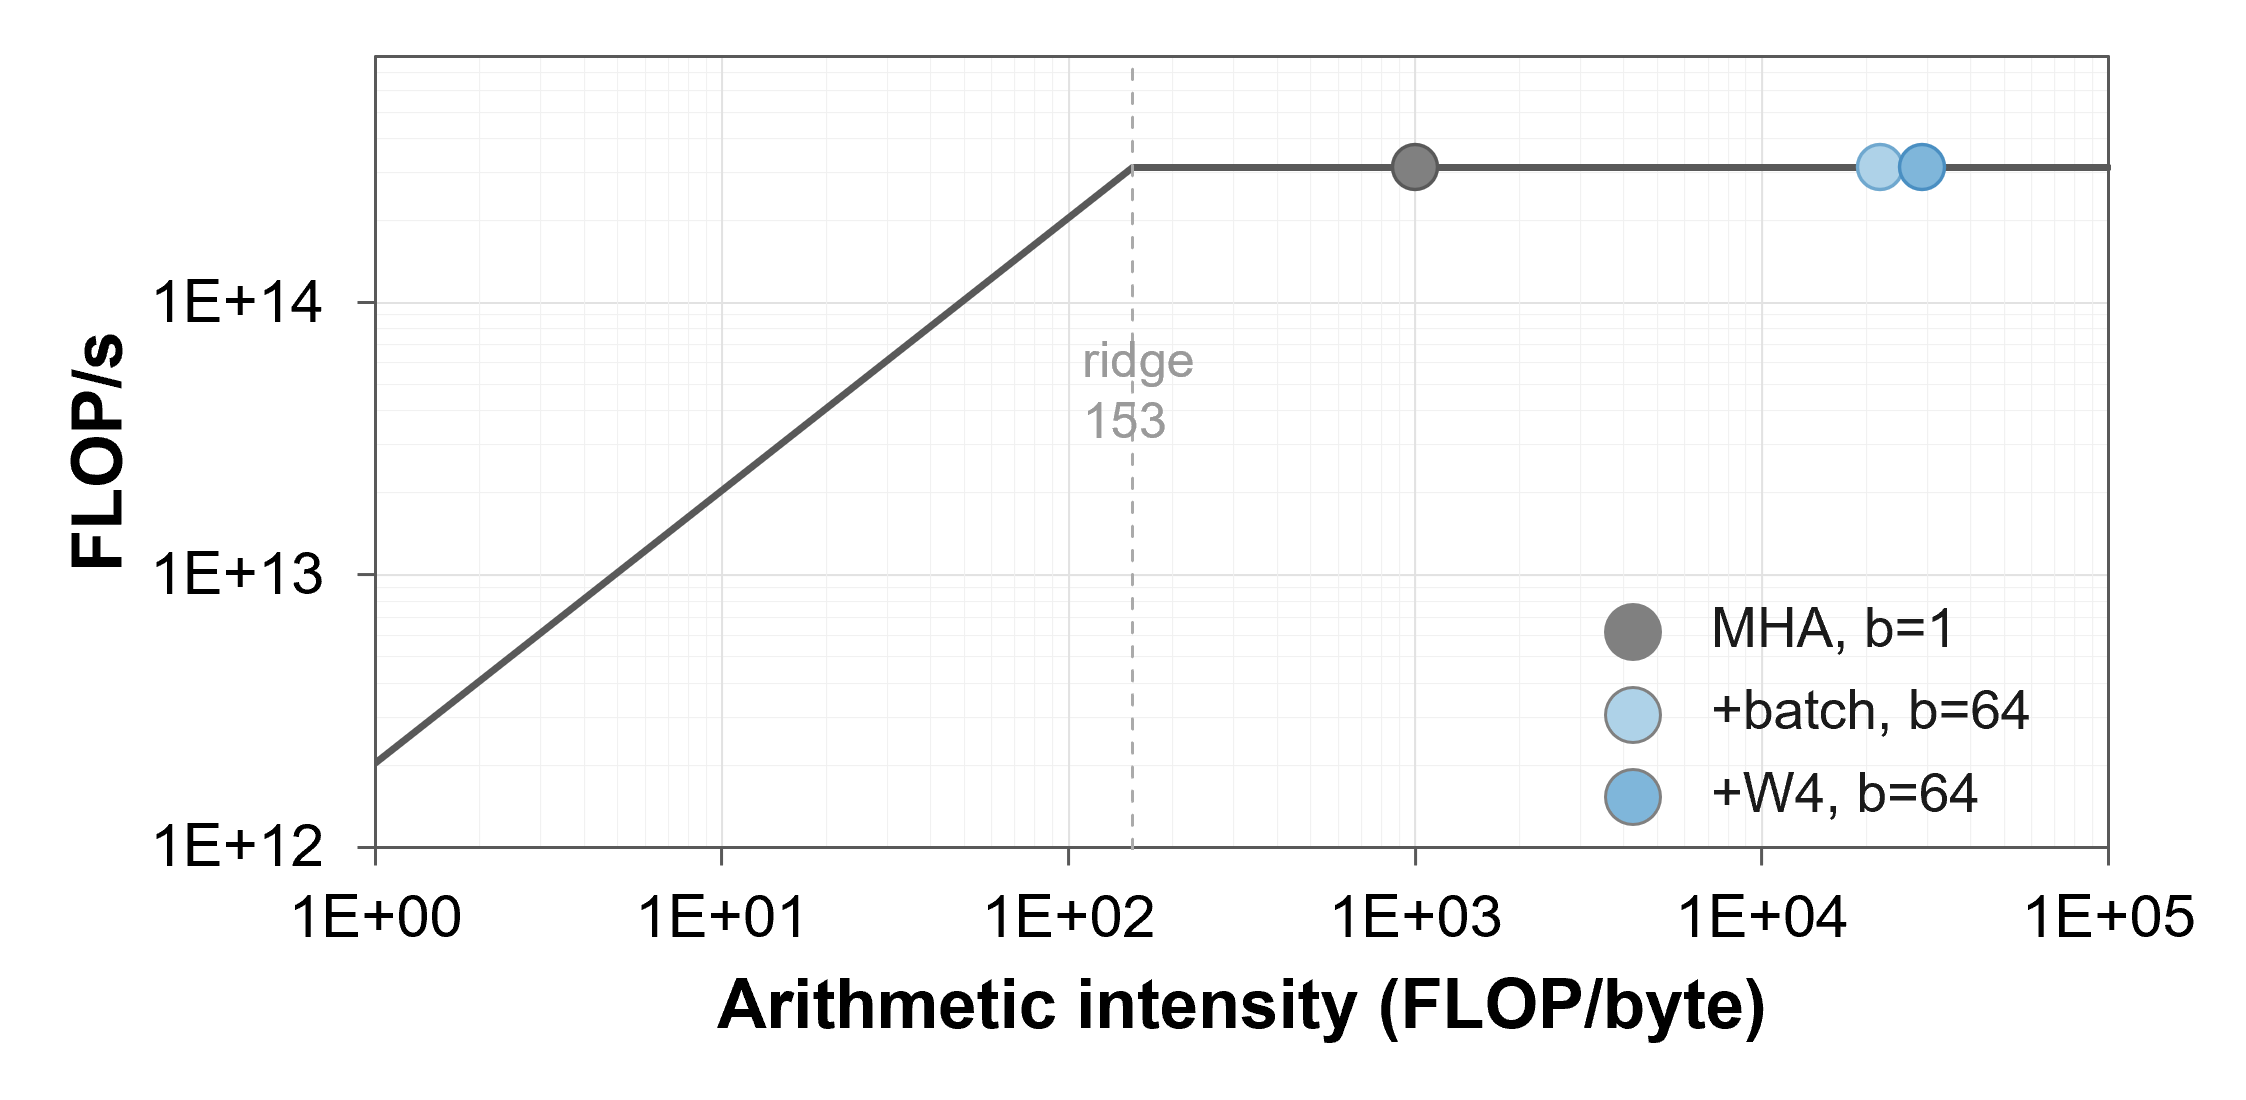
\includegraphics[width=0.92\linewidth]{figures/roofline_prefill.png}
        \caption{Prefill with a sequence length of 1024.}
        \label{fig:roofline_prefill}
    \end{subfigure}
    \caption{A100 FP16 roofline with a peak throughput of 312~TFLOP/s and a ridge point of 153~FLOP/byte. Decode configurations progressively apply batch scaling, GQA, MLA, weight quantization, and KV-cache quantization, while prefill configurations apply batch scaling and weight quantization.}
    \label{fig:bottleneck-analysis}
\end{figure}

\subsection{Limitations of Software-based FP-INT Execution}

Software \fpint{} GEMM kernels keep weights quantized in memory and fuse dequantization into the GEMM. Existing GPU Tensor Cores, however, do not natively support GEMMs between FP activations and INT operands. Each INT value must therefore be converted to FP before multiplication, and the dot product still executes on an FP$\times$FP Tensor Core. Fusion can hide much of the conversion latency, so dequantization latency itself is not the fundamental energy limitation. The fundamental limitation is that every MAC still incurs the cost of the FP$\times$FP datapath. Software optimization therefore captures the memory benefit of quantization but cannot exploit the substantially higher compute density and energy efficiency of a dedicated \fpint{} unit~\cite{figna}.

\subsection{System-Level Limitations of Existing FP-INT Accelerators}
\label{sec:sys_gap}

Prior \fpint{} hardware studies use custom arrays or lookup-table-based units to execute \fpint{} products efficiently. FIGNA~\cite{figna} aligns FP mantissas to a shared exponent and performs the dot product with integer MACs, whereas FIGLUT~\cite{figlut} and LUT Tensor Core~\cite{lut_tensor_core} exploit low-bit weight patterns to replace multiplications with table lookups and accumulation. These techniques eliminate the conventional dequantize-then-FP-MAC path and improve array-level TOPS/mm$^2$ and TOPS/W. However, two system-level limitations remain before these gains translate into end-to-end LLM-inference performance.

\textbf{Limitation 1: Existing \fpint{} datapaths do not natively support all quantized-attention mappings.}
KV-cache quantization associates scale and zero-point metadata with either tokens or channels of the original K and V tensors. We refer to these quantization directions as token-wise and channel-wise quantization, respectively. Quantization group size separately specifies how many elements share each metadata entry. The selected direction differs across frameworks, and the same K or V tensor may be quantized along different axes in different schemes, as summarized in Table~\ref{tab:kv_quant_direction}~\cite{liu2024kivi,hooper2024kvquant,he2024zipcache,yue2024wkvquant,duanmu2024skvq,ashkboos2024quarot,liu2024spinquant}.

Quantized attention performs the same $QK^T$ and $PV$ arithmetic in prefill and decode. Decode applies each new query to an INT KV cache that grows with sequence length, while prefill applies all query tokens to the context and incurs an attention workload that grows as $O(N^2)$. Falling back to an FP attention path therefore loses the compute- and energy-efficiency benefits of KV-cache quantization in both stages, particularly as attention becomes a substantial portion of long-sequence prefill latency, as shown in Figure~\ref{fig:long_seq_atten_overhead}. Most prior \fpint{} designs focus on linear-layer GEMMs and leave quantized attention on the conventional FP path. AxCore considers quantized attention but does not natively support token-wise KV quantization~\cite{axcore}.

\begin{figure}[t]
    \centering
    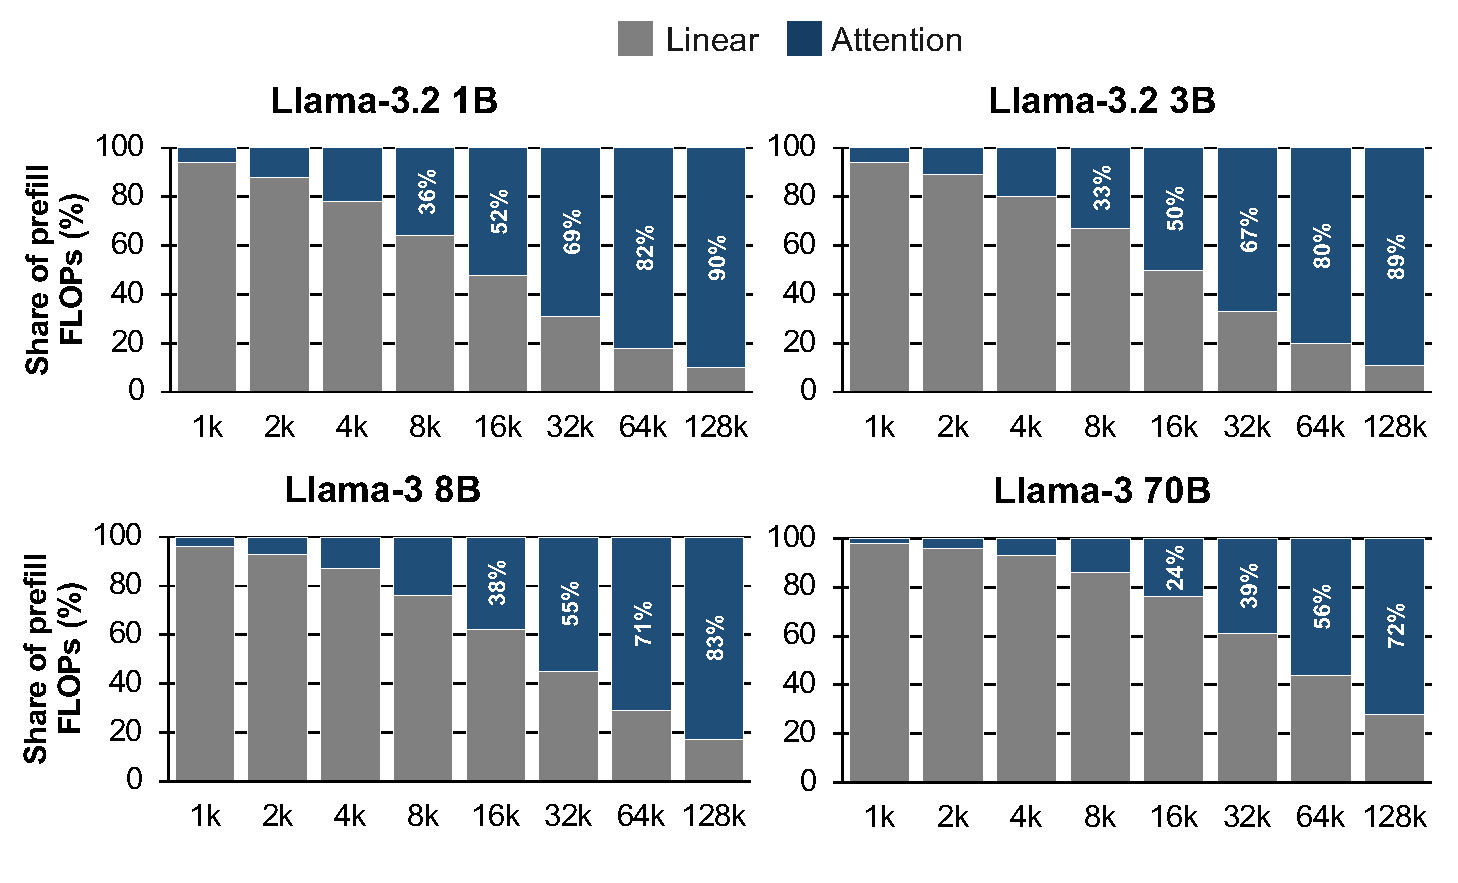
\includegraphics[width=0.92\linewidth]{figures/long_seq_attn_breakdown.pdf}
    \caption{Accelerating attention during prefill becomes critical in the long-sequence regime.}
    \label{fig:long_seq_atten_overhead}
\end{figure}

\begin{table}[t]
\centering
\caption{Quantization directions used by KV-cache quantization schemes.}
\label{tab:kv_quant_direction}
\small
\setlength{\tabcolsep}{3pt}
\begin{tabularx}{\columnwidth}{@{}>{\raggedright\arraybackslash}Xcc@{}}
\toprule
Scheme & K Direction & V Direction \\
\midrule
KIVI / KVQuant / ZipCache & channel-wise & token-wise \\
WKVQuant / SKVQ / QuaRot / SpinQuant & token-wise & token-wise \\
\bottomrule
\end{tabularx}
\end{table}

The hardware-level quantization direction depends on how the quantized tensor is mapped into a GEMM. When a quantized weight or KV tensor is consumed as the INT operand of a GEMM, we define its hardware quantization direction with respect to the operand layout seen by the MXU. We call it \qcol{} when the scale and zero-point metadata are associated with columns of the INT operand, and \qrow{} when they are associated with rows. These hardware directions are distinct from the token-wise and channel-wise quantization directions of the original K and V tensors. Their mapping depends on the attention operation and whether the INT operand is consumed in its standard or transposed orientation.
For example, consuming a channel-wise-quantized K tensor in transposed orientation for QK$^T$ maps its metadata along the GEMM reduction dimension. Token-wise quantization of V similarly places metadata along the reduction dimension of PV. Both cases therefore require \qrow{} execution.
A conventional \qcol{} datapath cannot factor a single scale and zero-point correction out of these dot products and must instead apply per-term dequantization before an FP reduction, erasing much of the intended efficiency, as illustrated in Figure~\ref{fig:quant_row_dir_overhead}.

\begin{figure}[t]
    \centering
    \begin{subfigure}[t]{\linewidth}
        \centering
        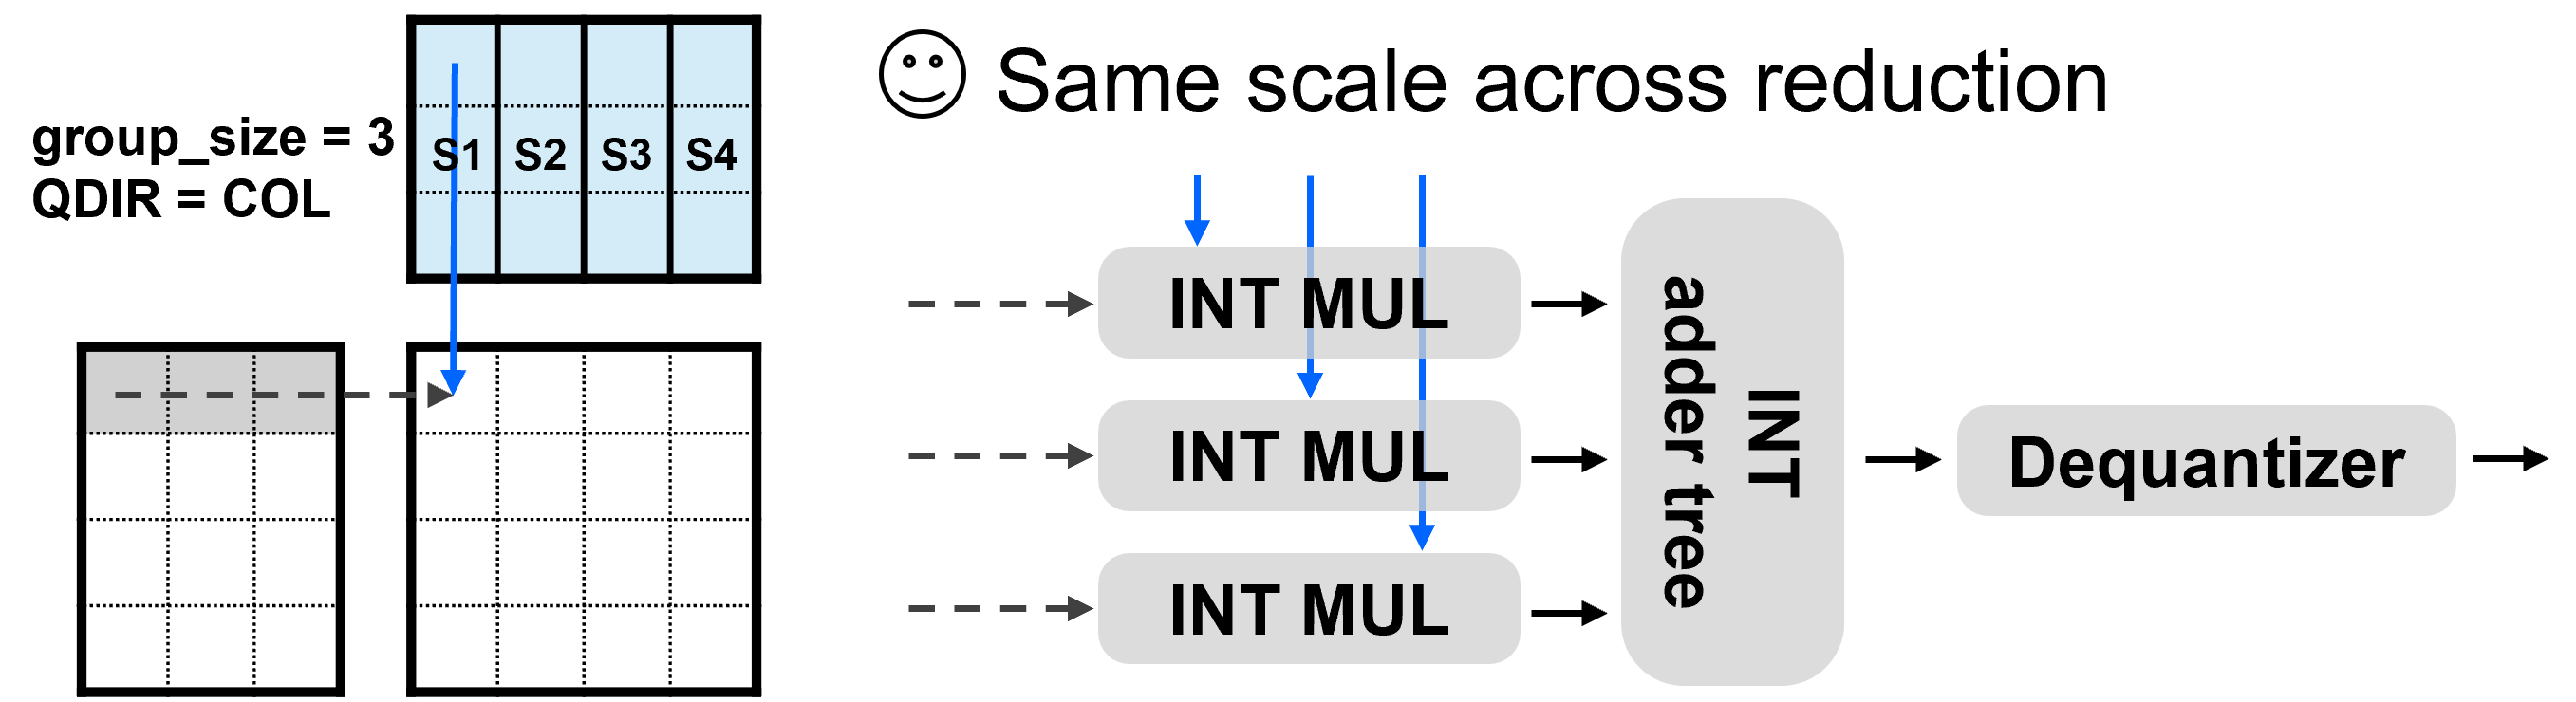
\includegraphics[width=0.92\linewidth]{figures/fig4_a.png}
        \caption{\qcol{} execution on a conventional FIGNA-style datapath.}
        \label{fig:conv_acc}
    \end{subfigure}
    \vspace{0.5em}
    \begin{subfigure}[t]{\linewidth}
        \centering
        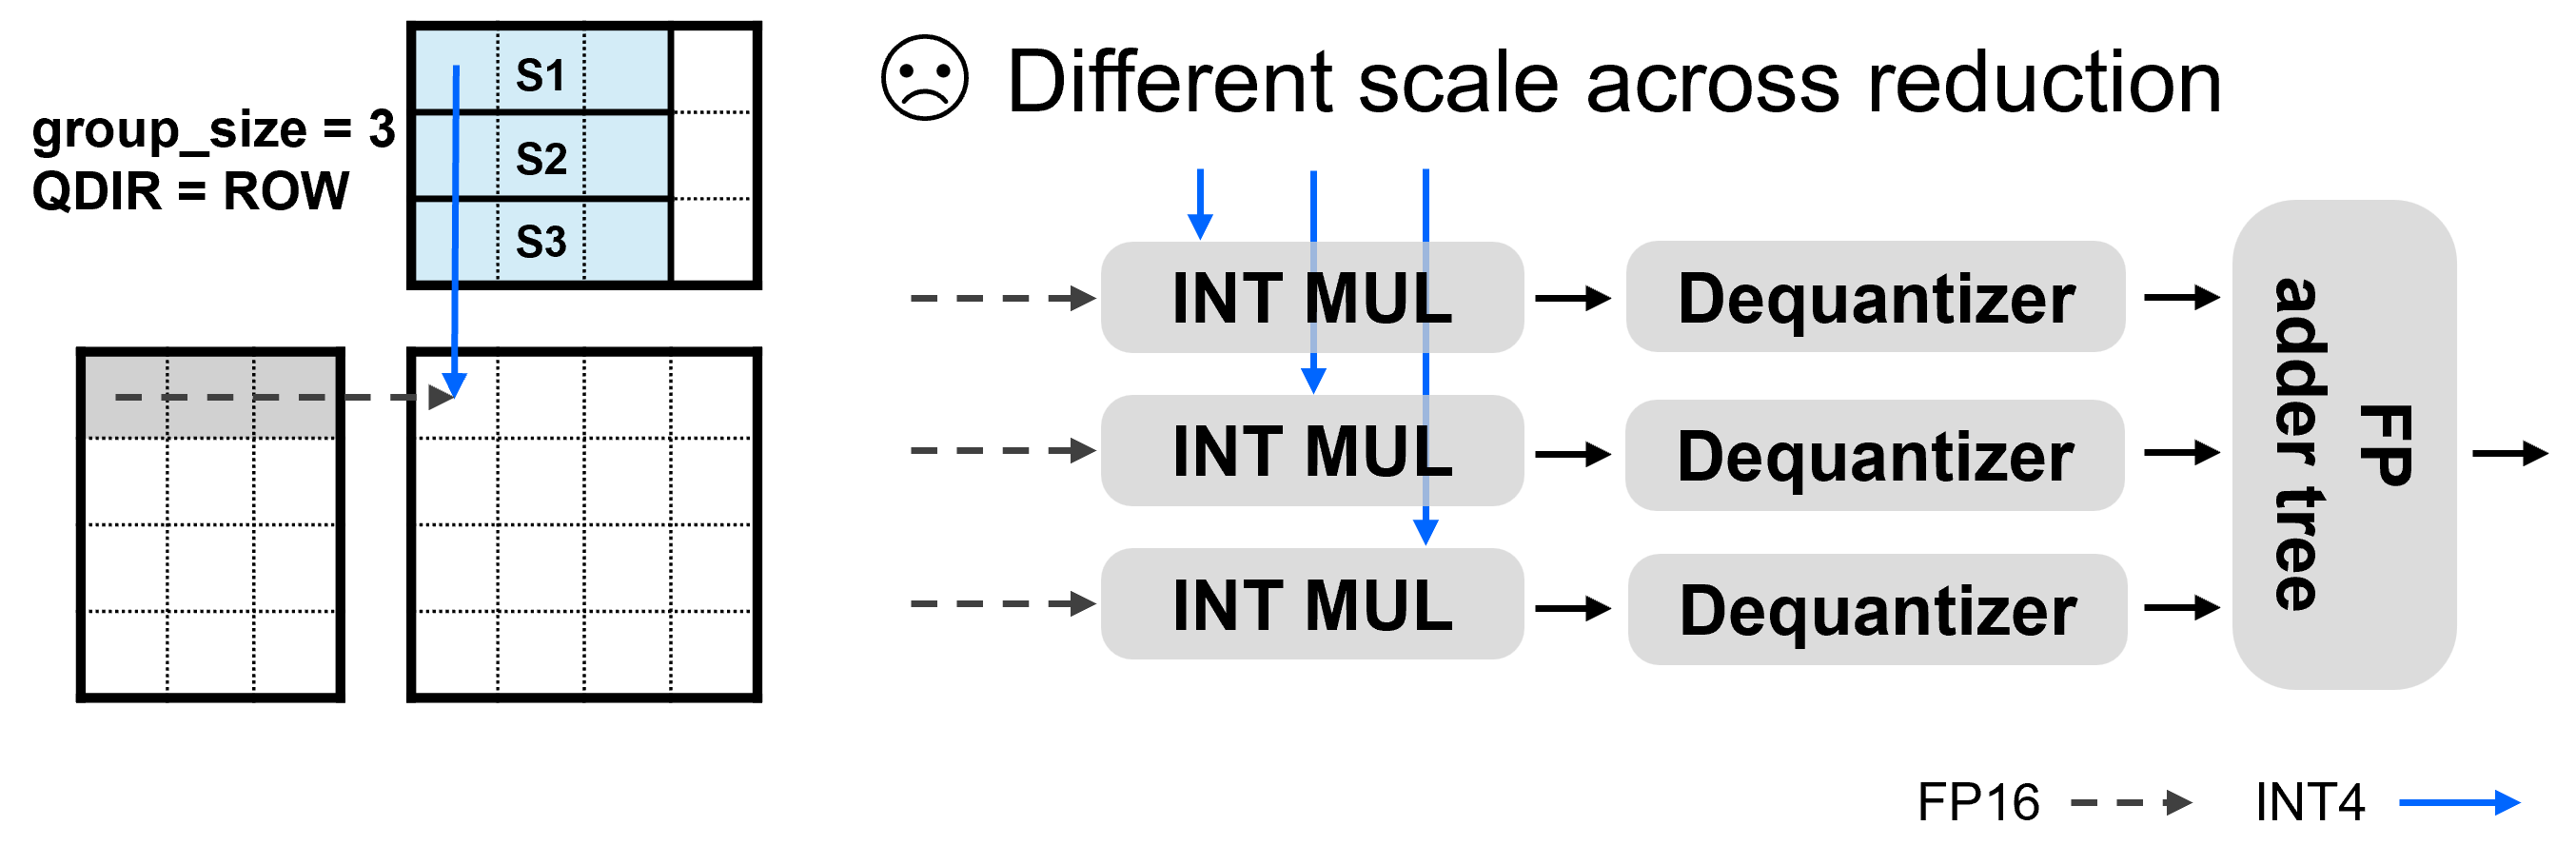
\includegraphics[width=0.92\linewidth]{figures/fig4_b.png}
        \caption{\qrow{} execution on a datapath designed only for \qcol{}.}
        \label{fig:row_quant}
    \end{subfigure}
    \caption{\qrow{} introduces per-term dequantization and FP-reduction overhead on an accelerator designed only for \qcol{}.}
    \label{fig:quant_row_dir_overhead}
\end{figure}

\textbf{Limitation 2: General-purpose operand-delivery paths diminish the avdantage of increased array-level density.}
A larger \fpint{} MXU improves performance only when the system can keep it supplied with operands and partial sums. Prior \fpint{} accelerator work emphasizes array-level efficiency, but system-level throughput also depends on memory bandwidth, command bandwidth, and low-latency tensor transfers.

Conventional GPU-style memory hierarchies preserve flexible access across local memory, cache, and the register file through heavily connected crossbars~\cite{jin2024uncovering,tine2021vortex}. Replacing an FP$\times$FP MXU with a larger \fpint{} MXU while proportionally scaling this crossbar-based structure causes interconnect and peripheral costs to grow rapidly with port and bank counts. As Figure~\ref{fig:xbar_overhead} shows, these costs can substantially diminish the array-level TOPS/mm$^2$ advantage of \fpint{} computation.

\begin{figure}[t]
    \centering
    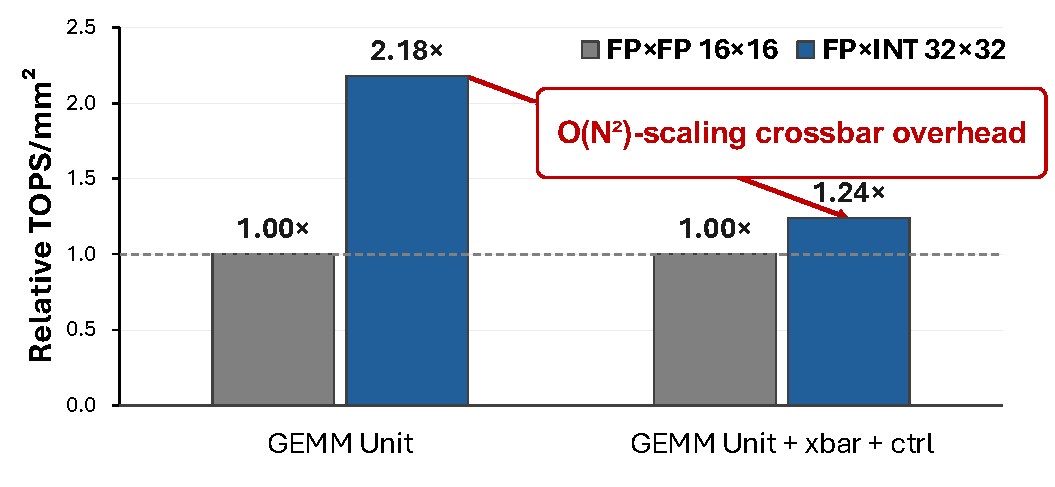
\includegraphics[width=0.82\linewidth]{figures/fig5.pdf}
    \caption{Relative TOPS/mm$^2$ of FP$\times$FP and \fpint{} GEMM units as crossbar and memory-system areas are progressively included. To match the ridge point of the GEMV roofline, the local-memory bank count increases from 16 to 64, the data-cache bank count from 2 to 8, and the number of HBM access ports from 2 to 8.}
    \label{fig:xbar_overhead}
\end{figure}

These limitations motivate a system that combines native support for both \qcol{} and \qrow{} attention, a specialized tensor-memory path that sustains the denser \fpint{} MXU, and software support that satisfies the resulting layout and placement constraints.

%Jae-Joon
\begin{comment}
\iffalse
\subsection{WKV Quantized LLM Inference}

The main operations of LLM inference consist of the Q/K/V linear projections, the attention score computation ($QK^T$), the attention-value product ($PV$), the $O$ linear projection, and the FFN layer. Under weight-only quantization, the linear projections and the MLP layer turn into products of an FP activation and an INT weight. Once KV-cache quantization is also applied, the $K$ and $V$ matrices of attention are stored in INT as well, so both attention GEMMs likewise become \fpint{} operations: $QK^T$ pairs an FP $Q$ with an INT $K$, and $PV$ pairs an FP probability with an INT $V$.

Letting $S_*$ and $Z_*$ denote the quantization scale and zero point, the compute kernels of \wkv{} quantized inference can be summarized as follows:
\begin{align}
    Y_{\mathrm{linear},fp}
    &= X_{fp} \left( (W_{int} - Z_W) \odot S_W \right), \\
    P_{fp}
    &= \mathrm{softmax}\left(
        \frac{
        Q_{fp} \left( (K_{int} - Z_K) \odot S_K \right)^T
        }{\sqrt{d_k}}
    \right), \\
    O_{fp}
    &= P_{fp} \left( (V_{int} - Z_V) \odot S_V \right) .
\end{align}

Figure~\ref{fig:fpint_inference} contrasts the conventional GPU path with our target execution path. A conventional GPU dequantizes $W_{int}$, $K_{int}$, and $V_{int}$ before using an FP Tensor Core. \ours{} instead restructures scale/zero-point handling and dataflow so the same \fpint{} GEMM path natively consumes INT operands in both linear layers and the $QK^T$ and $PV$ attention kernels.

%\begin{figure}[t]
%    \centering
%    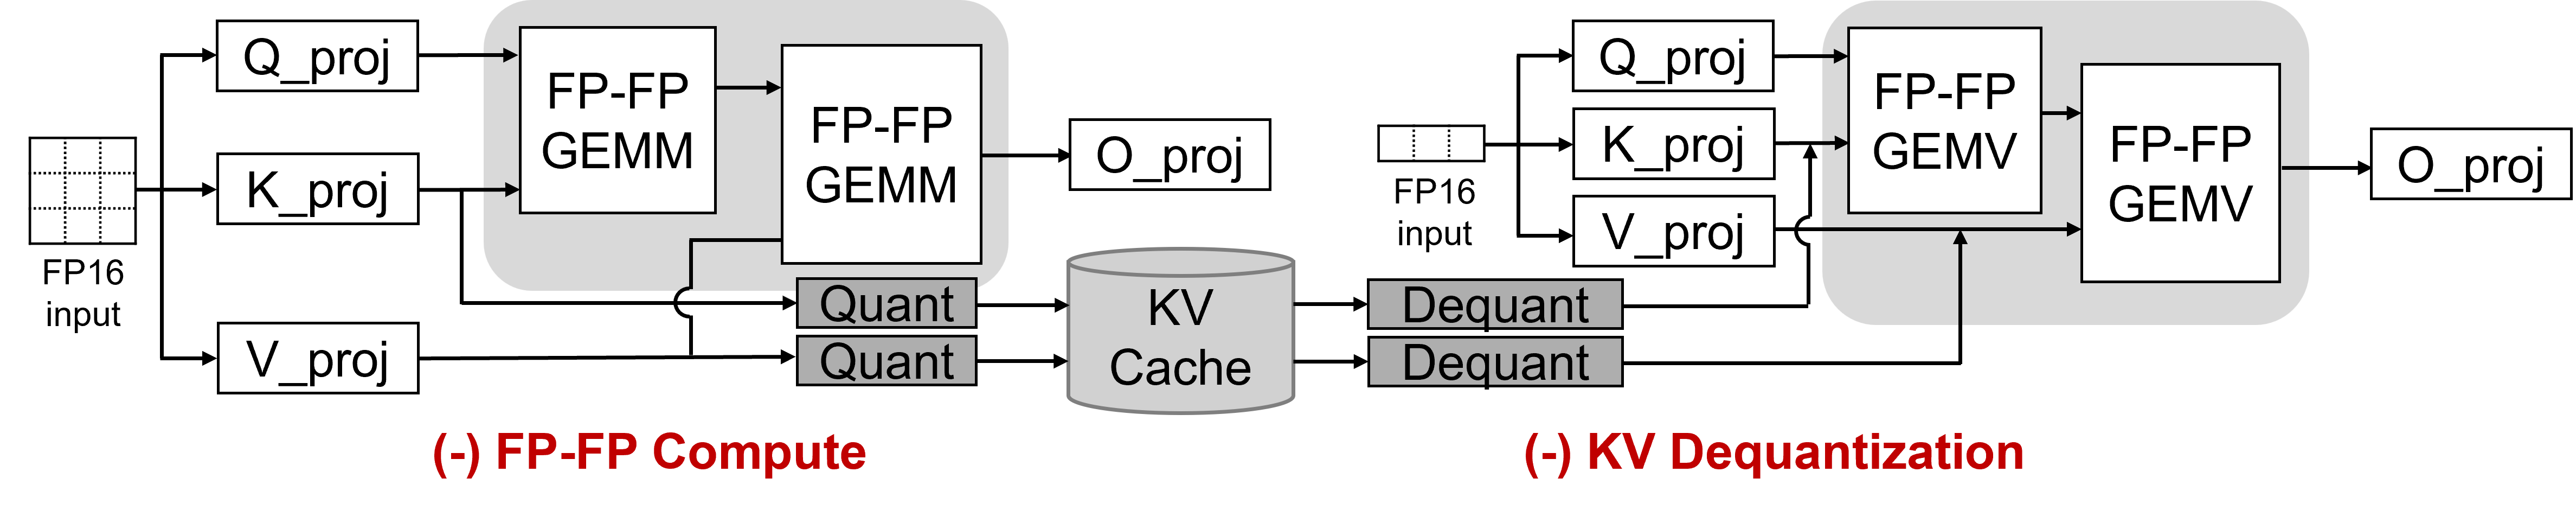
\includegraphics[width=0.98\linewidth]{figures/figs_fig1_2_a.png}
%    \caption{Execution paths for WKV quantized inference: (a) conventional GPU dequantizes INT weight/KV operands before FP GEMM, (b) prior \fpint{} hardware accelerates linear layers but leaves quantized KV attention on the FP path, and (c) our design executes both linear and attention GEMMs using native \fpint{} paths.}
    %\label{fig:fpint_inference}
%\end{figure}

\begin{figure}[t]
    \centering

    \begin{subfigure}[t]{\linewidth}
        \centering
        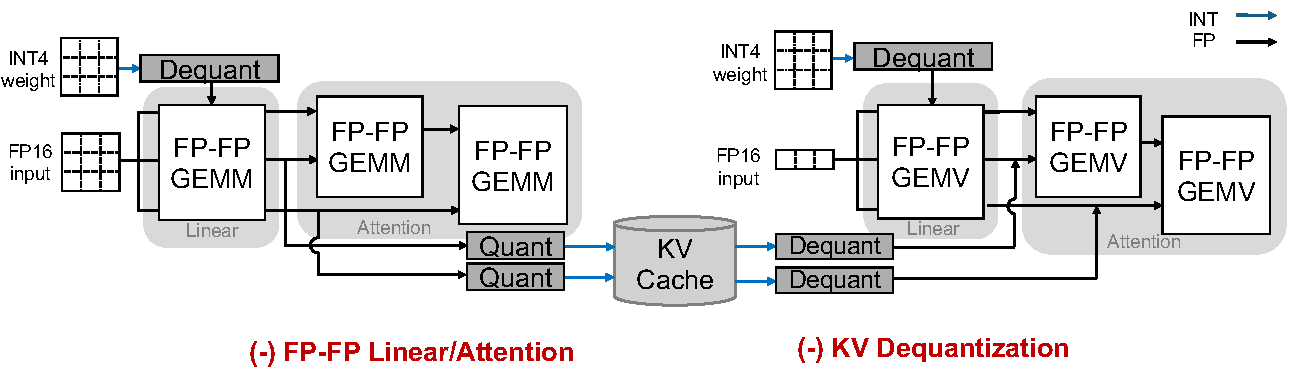
\includegraphics[width=0.95\linewidth]{figures/fig1_a.pdf}
        \caption{Conventional GPU dequantizes INT weight/KV operands before FP GEMM.}
        \label{fig:conventional gpu}
    \end{subfigure}

    \vspace{0.5em}

    \begin{subfigure}[t]{\linewidth}
        \centering
        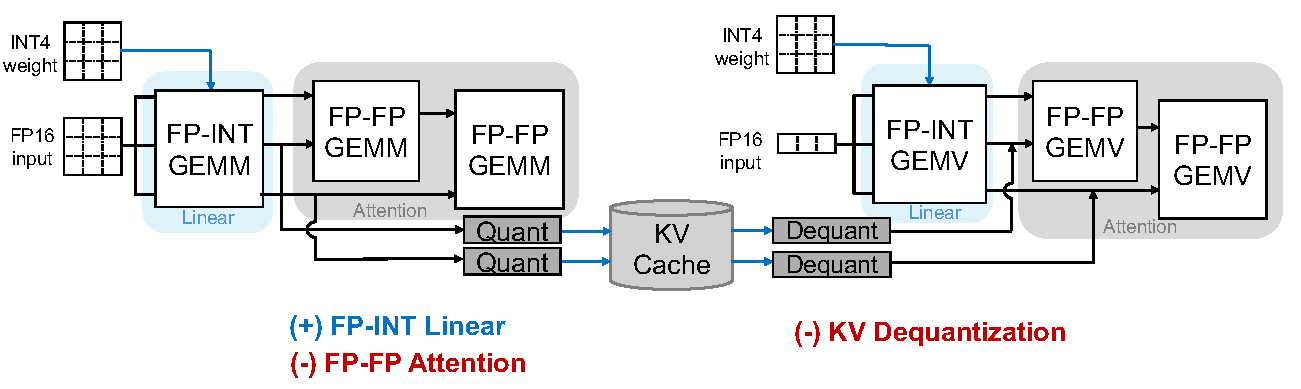
\includegraphics[width=0.95\linewidth]{figures/fig1_b.pdf}
        \caption{Prior FP-INT accelerators support only linear layers and leave attention on the FP path.}
        \label{fig:conventional gpu}
    \end{subfigure}

    \vspace{0.5em}

    \begin{subfigure}[t]{\linewidth}
        \centering
        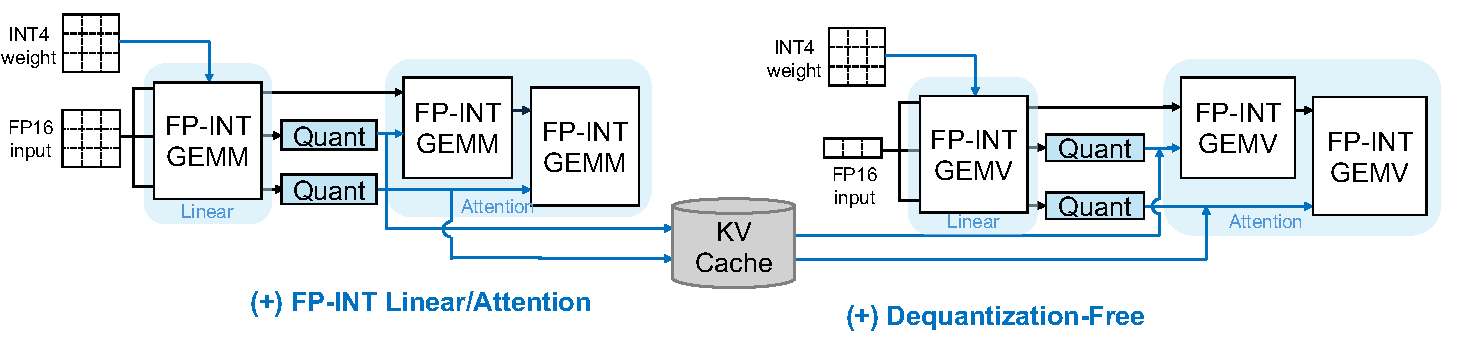
\includegraphics[width=0.99\linewidth]{figures/fig1_c.pdf}
        \caption{Our design executes both linear and attention GEMMs using native \fpint{} paths.}
        \label{fig:ours}
    \end{subfigure}

    \caption{Execution paths for WKV quantized inference.}
    \label{fig:fpint_inference}
\end{figure}


\subsection{Why Memory Saving Alone is Insufficient}

Quantization first reduces memory footprint, but it does not remove compute pressure. Prefill processes a prompt in one shot and is generally compute-bound. Decode is often memory-bound because it runs token by token and repeatedly reads the KV cache, yet GQA, MQA, MLA, batching, and quantization can push it closer to the compute-bound regime (Figure~\ref{fig:bottleneck-analysis}). Modern LLM serving therefore needs a datapath that processes quantized operands directly, rather than only reducing memory traffic and then dequantizing onto an FP unit.

% \begin{figure}[t]
%     \centering
%     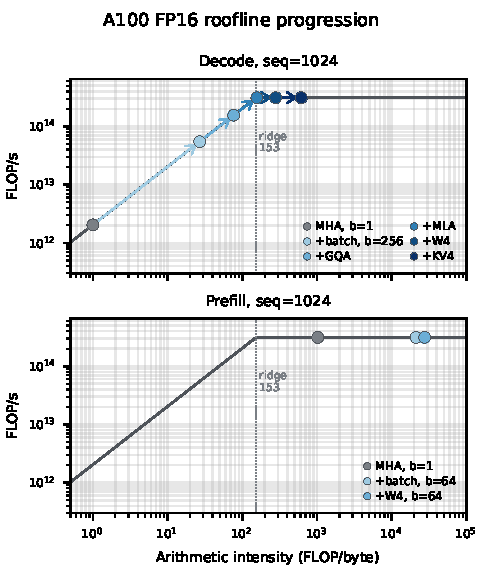
\includegraphics[width=0.92\linewidth]{figures/progression_roofline.pdf}
%     \caption{Memory traffic reduction alone becomes insufficient as arithmetic intensity increases.}
%     \label{fig:bottleneck-analysis}
% \end{figure}
\begin{figure}[t]
    \centering
    \begin{subfigure}[t]{\linewidth}
        \centering
        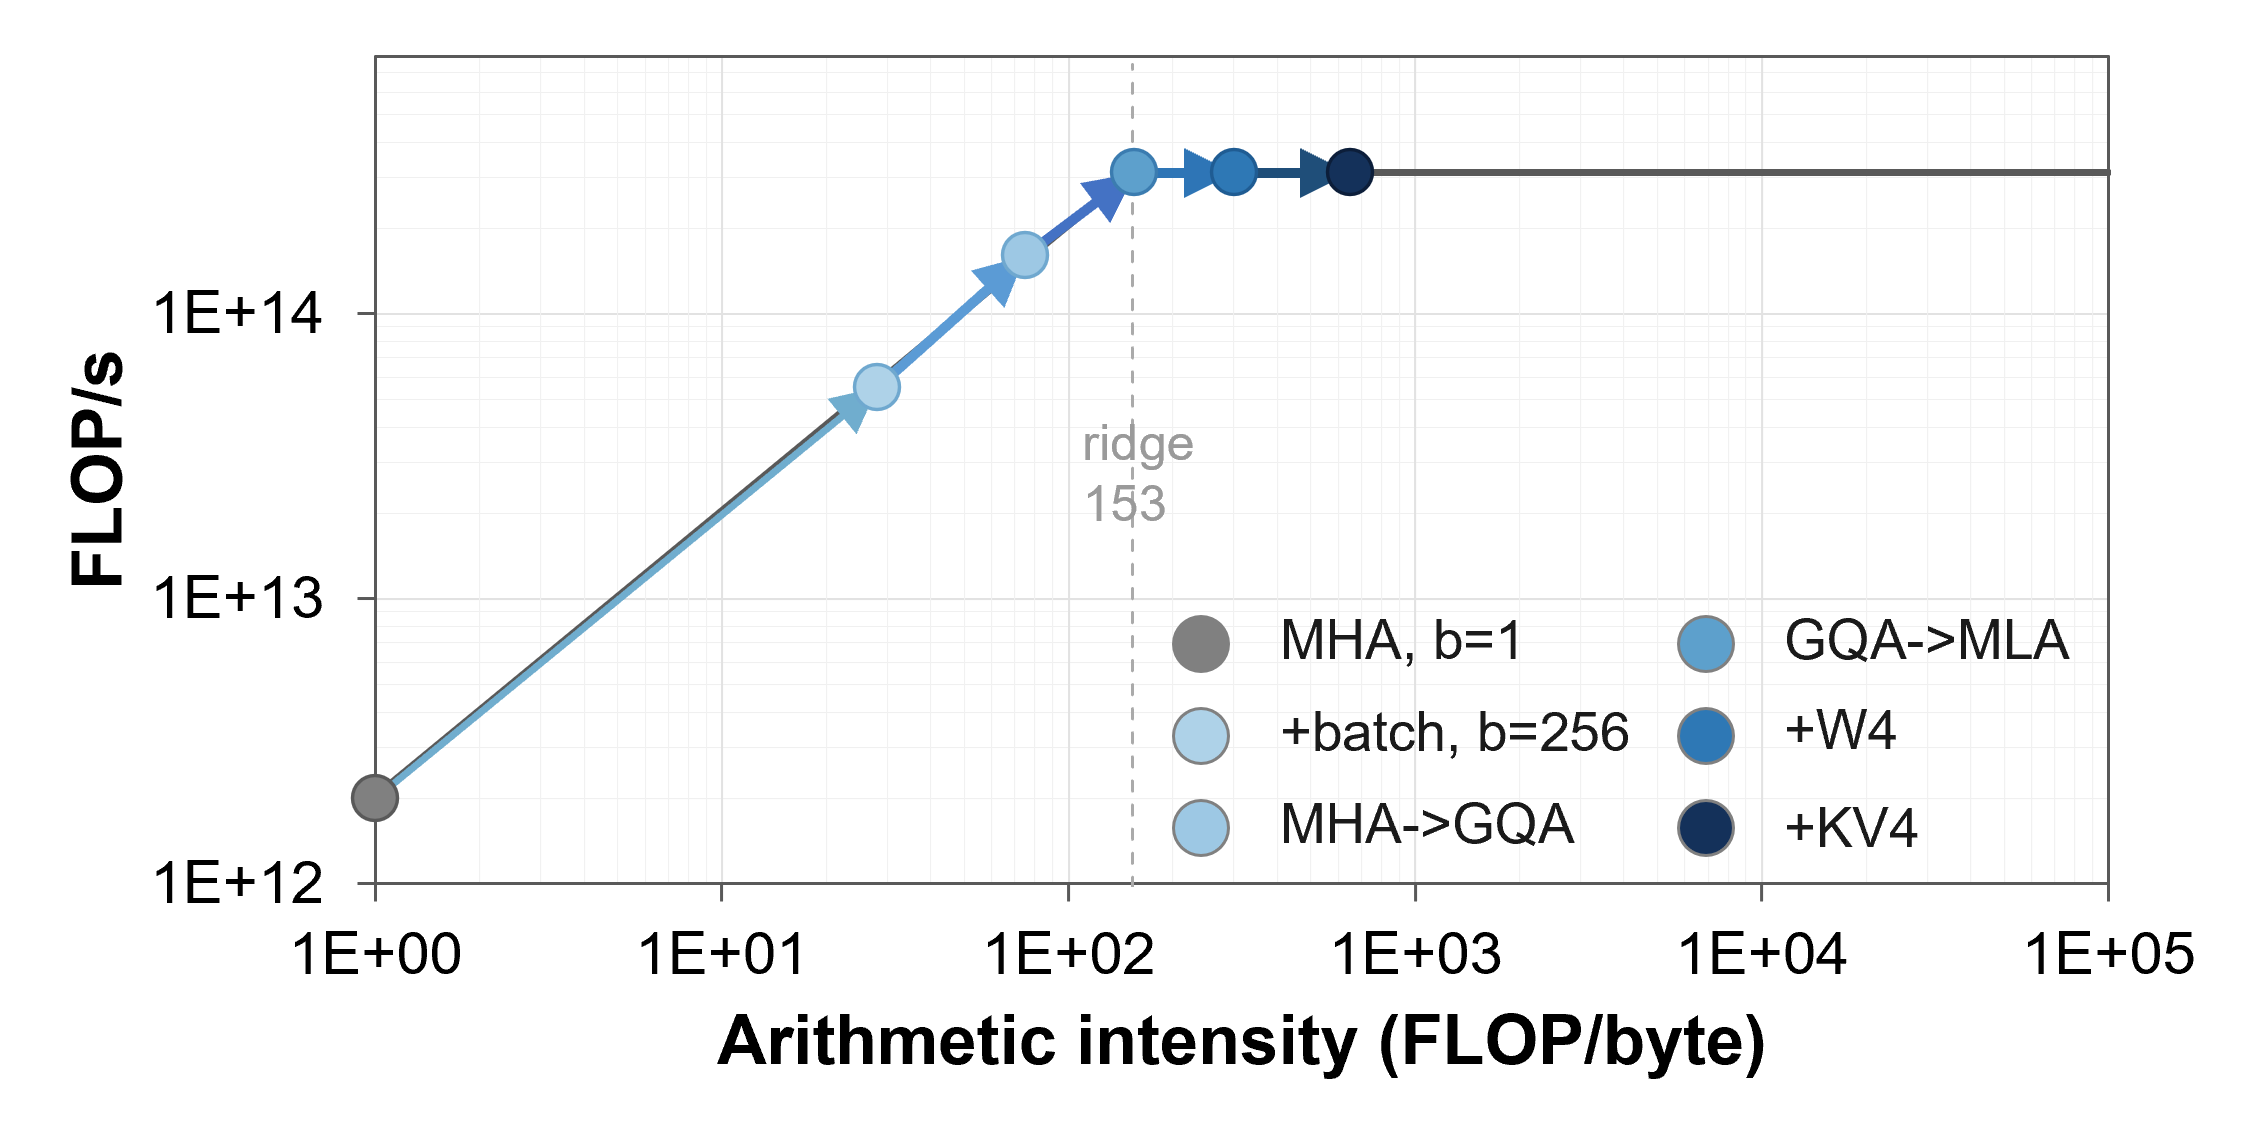
\includegraphics[width=0.8\linewidth]{figures/roofline_decode.png}
        \caption{Decode, sequence length of 1024}
        \label{fig:roofline_decode}
    \end{subfigure}
    \vspace{0.5em}
    \begin{subfigure}[t]{\linewidth}
        \centering
        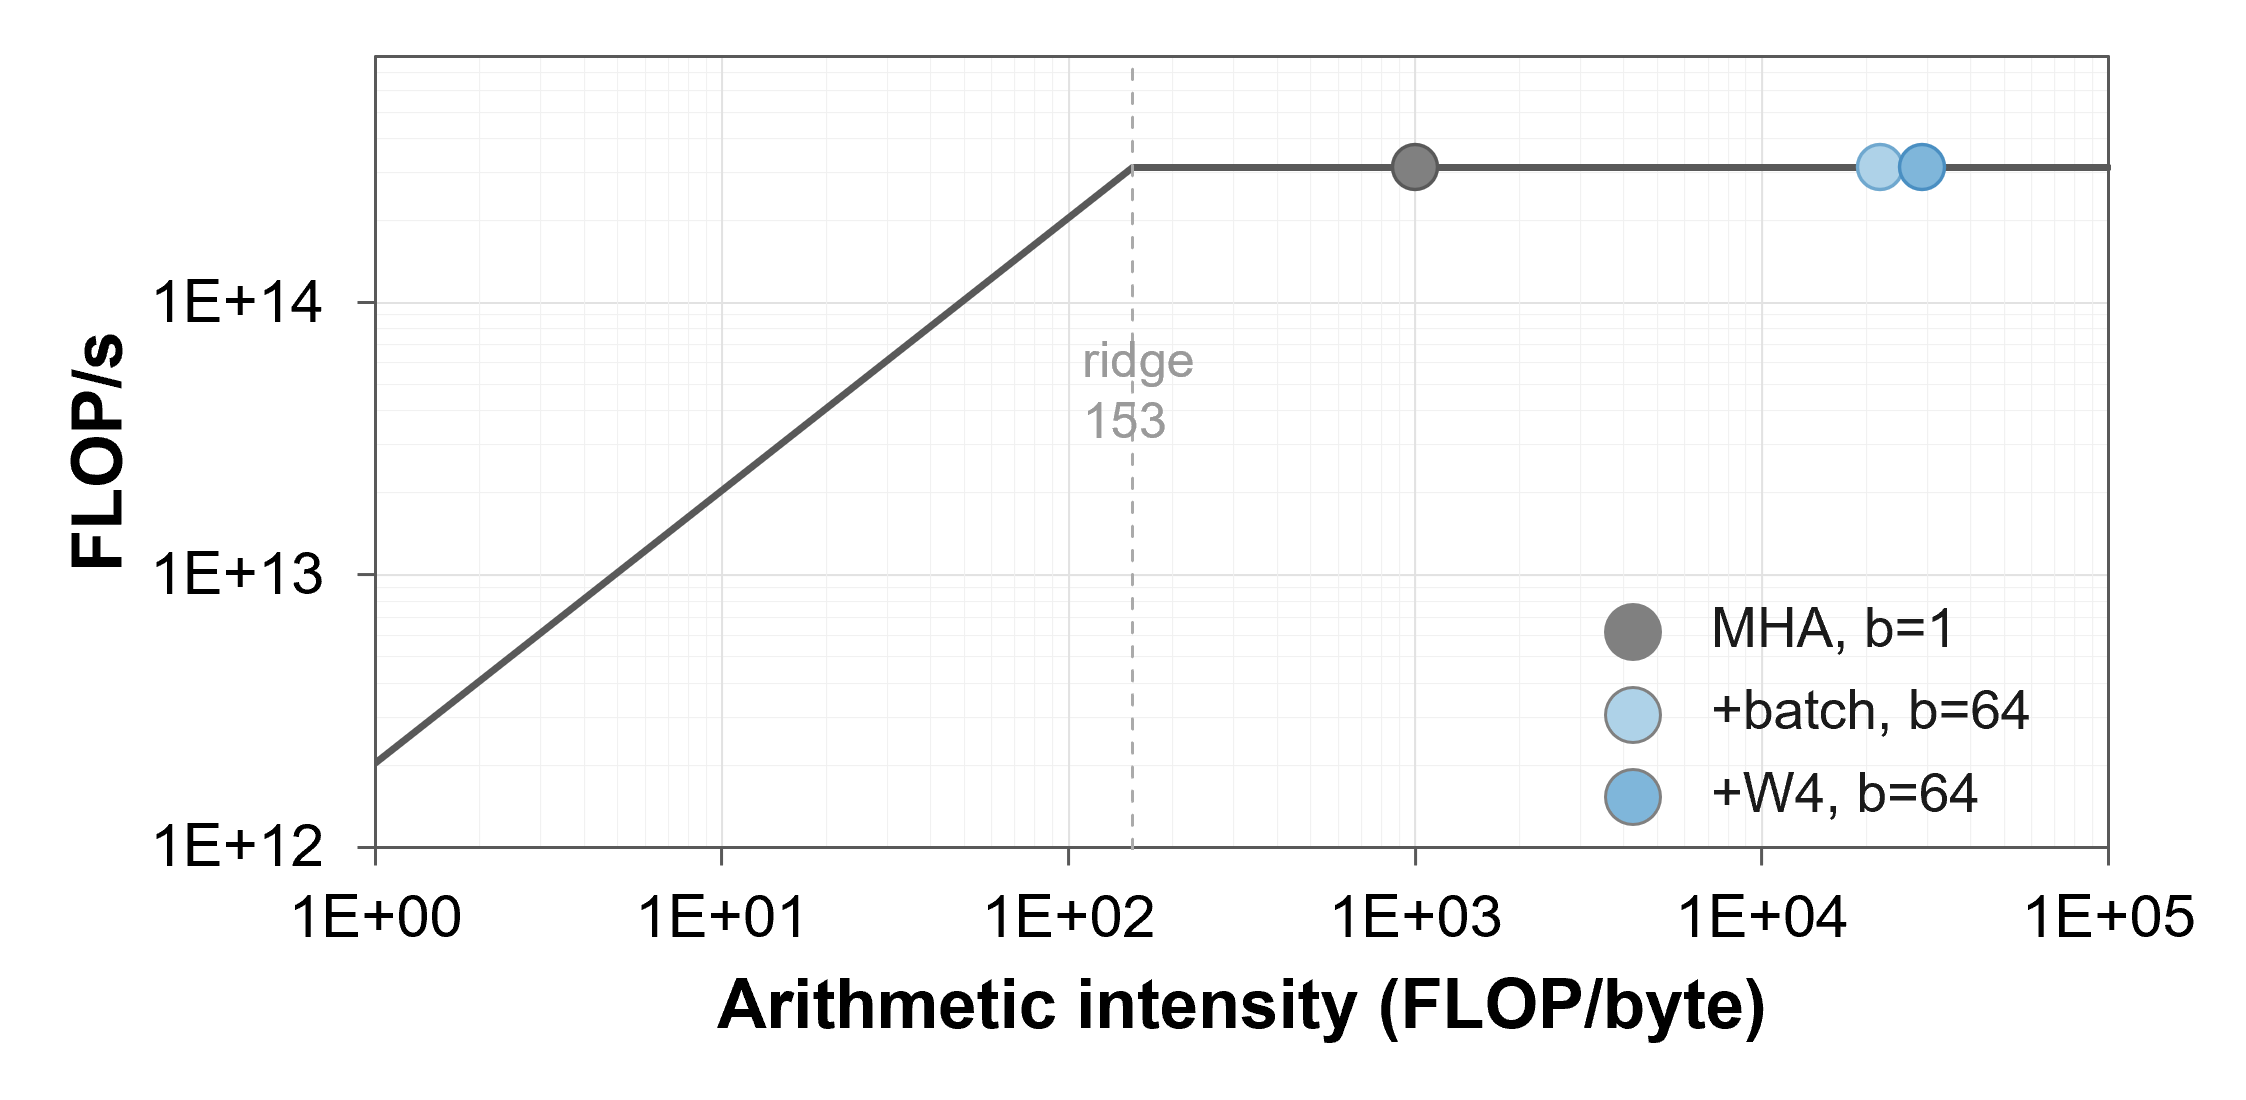
\includegraphics[width=0.8\linewidth]{figures/roofline_prefill.png}
        \caption{Prefill, sequence length of 1024}
        \label{fig:roofline_prefill}
    \end{subfigure}
    \caption{A100 FP16 roofline with a peak of 312~TFLOP/s and a ridge point at 153~FLOP/byte. For decode, the configurations progressively apply batch scaling, GQA, MLA, weight quantization, and KV quantization. For prefill, they apply batch scaling and weight quantization. 
    %These configurations raise arithmetic intensity beyond the ridge point, where reducing memory traffic alone no longer helps and compute path efficiency becomes the limiter. Prefill becomes compute bound even at modest batch sizes, while decode crosses the ridge as these configurations accumulate.
    }
    \label{fig:bottleneck-analysis}
\end{figure}



\subsection{Software FP-INT GEMM Optimization and Its Limitations}

Software \fpint{} GEMM kernels keep weights quantized in memory and fuse their dequantization into the GEMM. However, existing GPU Tensor Cores do not natively support GEMMs between FP activations and INT weights. Each INT weight must therefore be converted to FP before multiplication, and the dot product still executes on an FP$\times$FP Tensor Core. Fusion can hide much of the conversion latency, so dequantization itself is not the fundamental energy limitation. The fundamental limitation is that every MAC still incurs the energy cost of the FP$\times$FP datapath. Consequently, software optimization captures the memory benefit of quantization but cannot exploit the much higher compute-energy efficiency of a dedicated \fpint{} unit~\cite{figna}.

\subsection{Hardware FP-INT GEMM Accelerator and System-Level Gap}
\label{sec:sys_gap}

Prior \fpint{} hardware studies use custom arrays or lookup-table-based units to perform \fpint{} multiplications efficiently. 
They show high TOPS/mm$^2$ and TOPS/W at the array level.
They remove the conventional
dequantize-then-FP-MAC path by transforming the dot product into
a simpler datapath. FIGNA aligns FP mantissas to a shared exponent and
performs the dot product with integer MACs, whereas FIGLUT and LUT
Tensor Core exploit low-bit weight patterns to replace multiplications
with table lookups and accumulation~\cite{figna,figlut,lut_tensor_core}.
These transformations remove FP MAC and improve array-level compute density and energy efficiency.
But two gaps remain before these gains translate into end-to-end LLM-inference performance.

\textbf{Gap 1: Existing \fpint{} datapaths do not natively support quantized attention in both prefill and decode.}
KV cache schemes associate quantization metadata with either tokens or channels of the original K and V tensors before any transpose. We refer to these two quantization directions as token-wise and channel-wise, respectively. Quantization group size separately denotes the number of elements that share the metadata. Quantized attention executes the same $QK^T$ and PV operations in both stages. These operations therefore encounter the same \fpint{} arithmetic constraint. During decode, each new query attends to an INT KV cache that grows with the sequence length. Falling back to the FP path loses the computational and energy efficiency benefits of KV quantization. During prefill, all query tokens attend to the context. The attention workload therefore grows as $O(N^2)$ and becomes a substantial part of TTFT at long sequence lengths (Figure~\ref{fig:long_seq_atten_overhead}). Most prior \fpint{} designs focus on GEMMs in linear layers and leave quantized attention on the conventional FP path. AxCore considers quantized attention, but it does not natively support token-wise KV quantization~\cite{axcore}. Existing designs therefore cannot cover both token-wise and channel-wise KV quantization across $QK^T$ and PV. This limits their benefits in both prefill and decode.

\begin{figure}[t]
    \centering
    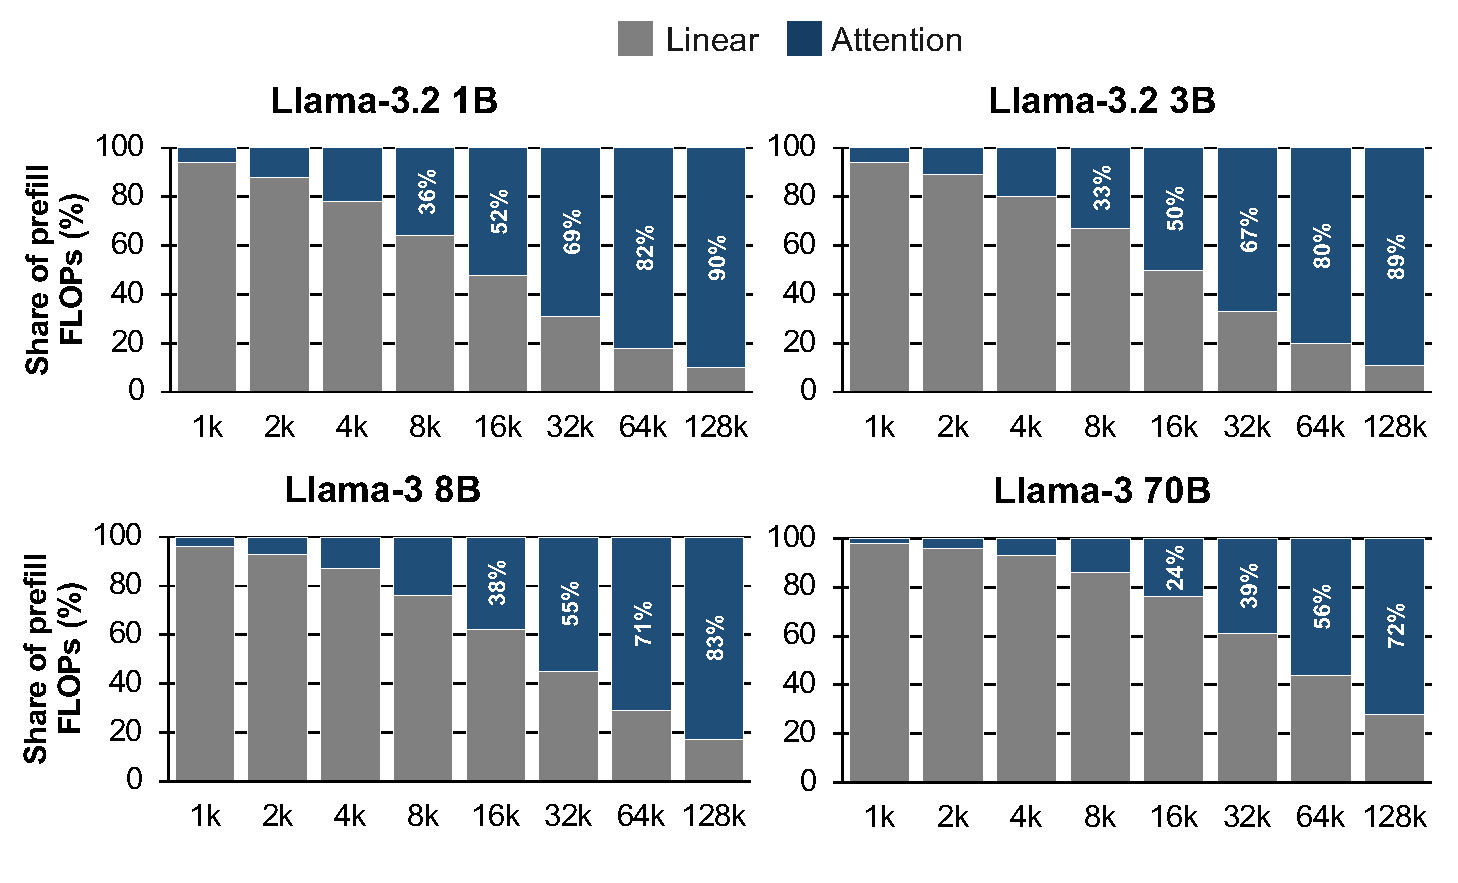
\includegraphics[width=0.92\linewidth]{figures/long_seq_attn_breakdown.pdf}
    \caption{Accelerating attention during prefill becomes critical in the long-sequence regime.}
    \label{fig:long_seq_atten_overhead}
\end{figure}

The underlying arithmetic limitation is common to both stages and comes from the direction of KV quantization metadata. Moving from prefill to decode changes the number of query rows, but does not change which tensor axis forms the reduction dimension in $QK^T$ and PV. Common KV quantization schemes use either token-wise or channel-wise quantization for K and V.
The selected direction varies across quantization frameworks. The same K or V tensor may use token-wise quantization in one framework and channel-wise quantization in another (Table~\ref{tab:kv_quant_direction})~\cite{liu2024kivi,hooper2024kvquant,he2024zipcache,yue2024wkvquant,duanmu2024skvq,ashkboos2024quarot,liu2024spinquant}.

\begin{table}[t]
\centering
\caption{Quantization directions used by KV cache quantization schemes.}
\label{tab:kv_quant_direction}
\small
\setlength{\tabcolsep}{3pt}
\begin{tabularx}{\columnwidth}{@{}>{\raggedright\arraybackslash}Xcc@{}}
\toprule
Scheme & K Direction & V Direction \\
\midrule
KIVI / KVQuant / ZipCache & channel-wise & token-wise \\
WKVQuant / SKVQ / QuaRot / SpinQuant & token-wise & token-wise \\
%- & channel-wise / token-wise & token-wise \\
\bottomrule
\end{tabularx}
\end{table}

After K is transposed for $QK^T$, channel-wise K metadata varies along the reduction dimension. Similarly, token-wise V metadata varies along the reduction dimension of PV. In either case, a conventional \fpint{} unit cannot factor out a single scale after the dot product. It must instead correct each term using its scale and zero point before accumulation and use an FP reduction. This erases much of the intended efficiency (Figure~\ref{fig:quant_row_dir_overhead}).
When an INT tensor is mapped to the right hand side (RHS) of a matrix multiplication unit (MXU), we call its quantization direction \qcol{} if metadata is associated with RHS columns and \qrow{} if metadata is associated with RHS rows. These hardware directions are distinct from the token-wise and channel-wise directions of the original K and V tensors. Their mapping depends on the attention operation and whether the RHS is transposed.

\begin{figure}[t]
    \centering

    \begin{subfigure}[t]{\linewidth}
        \centering
        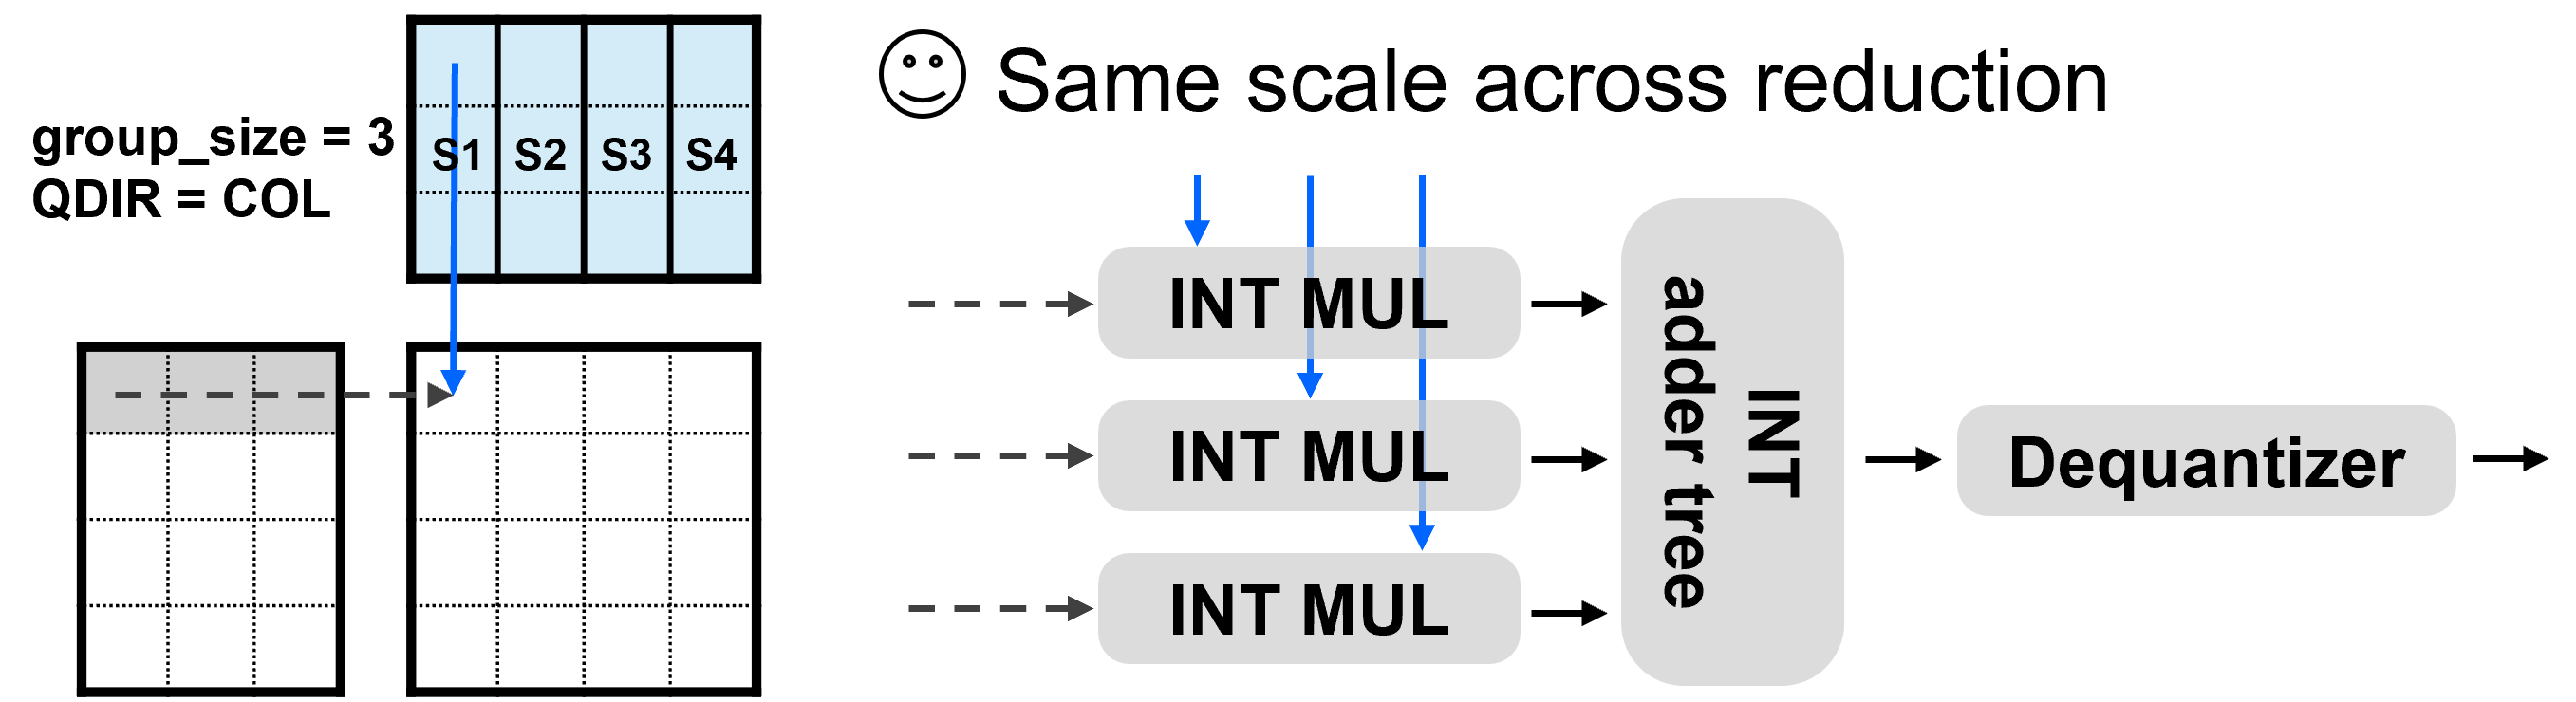
\includegraphics[width=0.92\linewidth]{figures/fig4_a.png}
        \caption{\qcol{} quantization direction (FIGNA style).}
        \label{fig:conv_acc}
    \end{subfigure}

    \vspace{0.5em}

    \begin{subfigure}[t]{\linewidth}
        \centering
        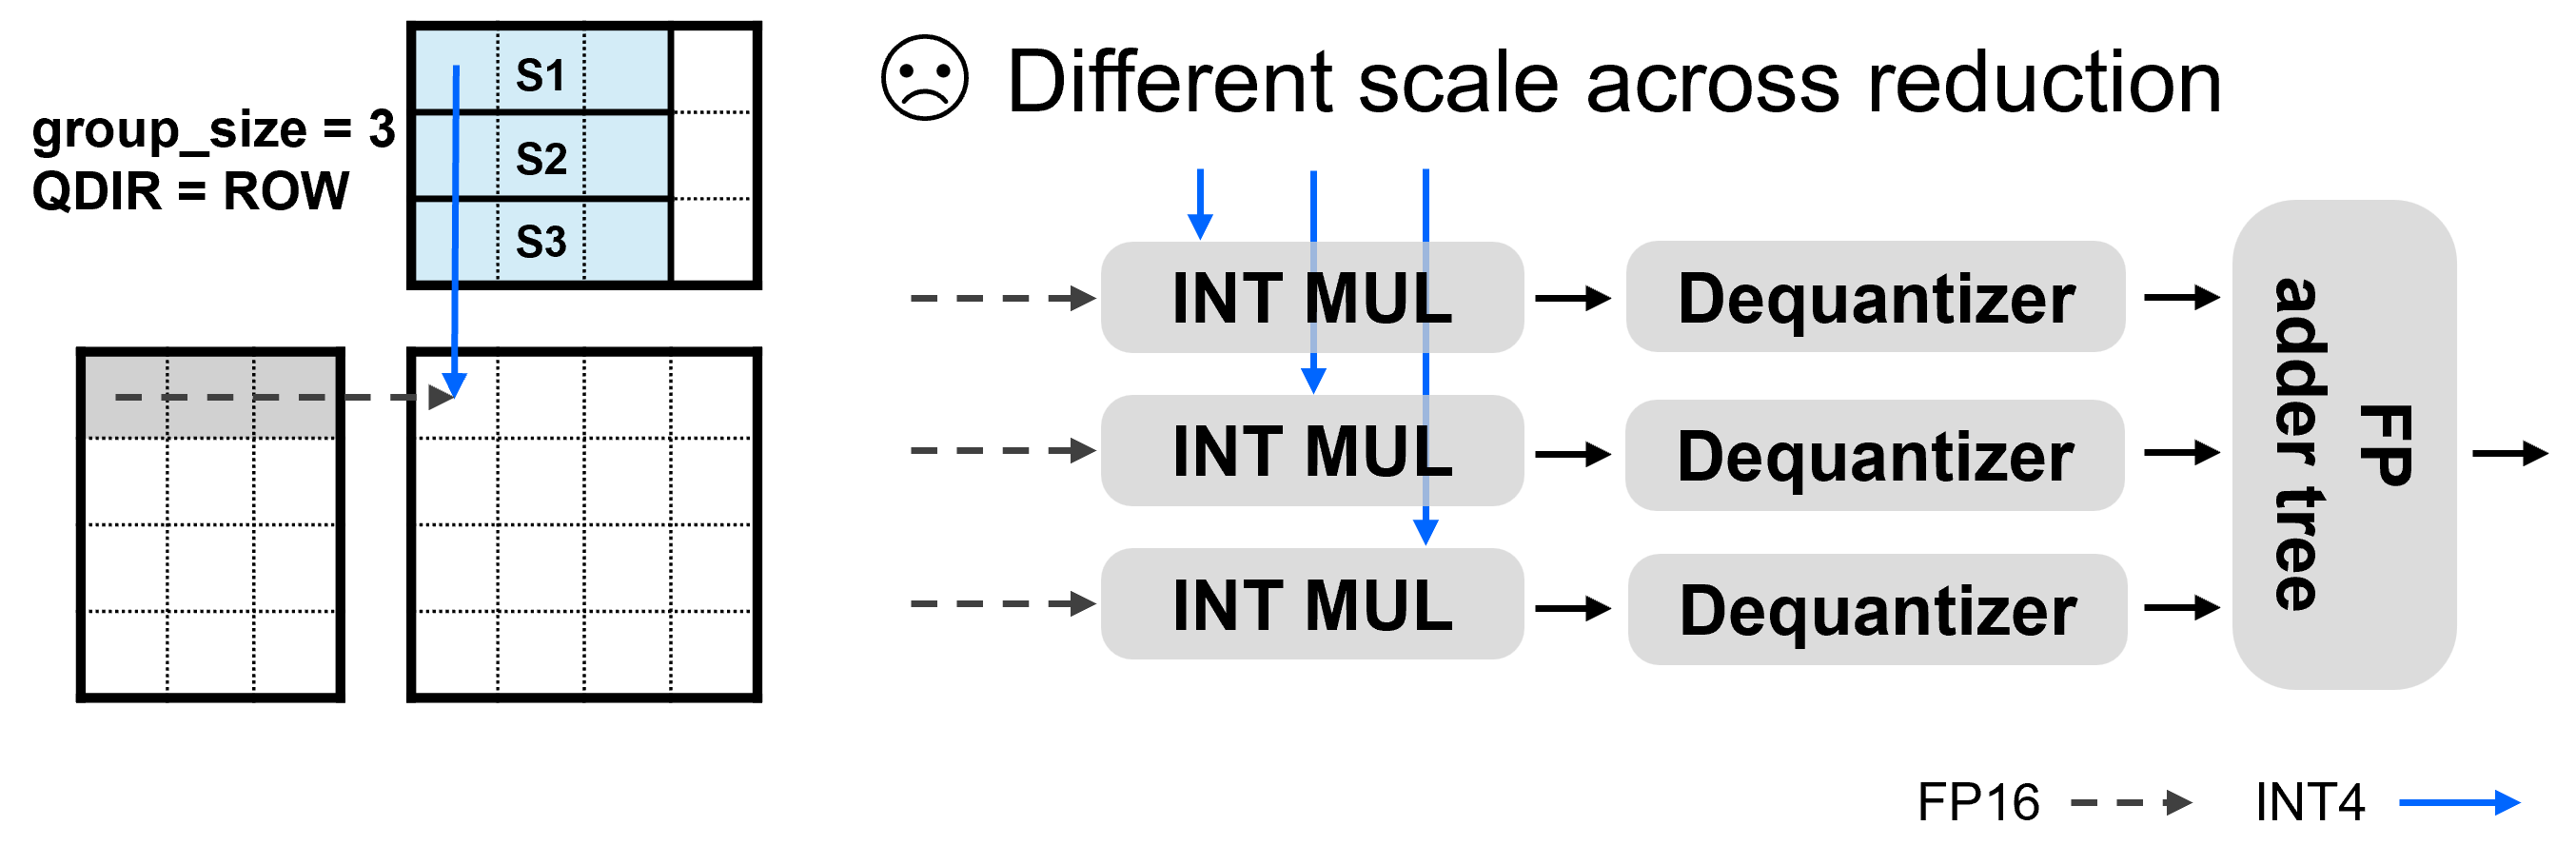
\includegraphics[width=0.92\linewidth]{figures/fig4_b.png}
        \caption{\qrow{} quantization direction on a conventional \qcol{} datapath.}
        \label{fig:row_quant}
    \end{subfigure}

    \caption{The \qrow{} quantization direction introduces overhead on an accelerator designed only for \qcol{}.}
    \label{fig:quant_row_dir_overhead}
\end{figure}

\textbf{Gap 2: A larger matrix unit alone does not guarantee performance gains.}
A larger \fpint{} MXU only helps if the system keeps it busy. Prior \fpint{} accelerator work focuses on array-level efficiency, but delivered TOPS also depends on memory bandwidth, command bandwidth, and low-latency bursts.

Scaling the memory subsystem is harder than increasing the bank count. Conventional GPU-style hierarchies expose flexible access across shared memory, cache, and the register file, so they rely heavily on crossbars~\cite{jin2024uncovering, tine2021vortex}. Replacing an FP$\times$FP MXU with a larger \fpint{} MXU while preserving this crossbar-based structure makes the interconnect cost grow as $O(N^2)$, which can erase the array-level TOPS/mm$^2$ advantage (Figure~\ref{fig:xbar_overhead}).

%Even after banking and interleaving provide raw bandwidth, the DMA must issue bursts whose per-cycle requests stay within bank boundaries. Misaligned accesses require a barrel shifter that scales with DMA width, adding area, power, and timing cost. Thus the system must scale bandwidth while also constraining layout and access patterns enough for simple, aligned bursts.

%\begin{figure}[t]
%    \centering
%    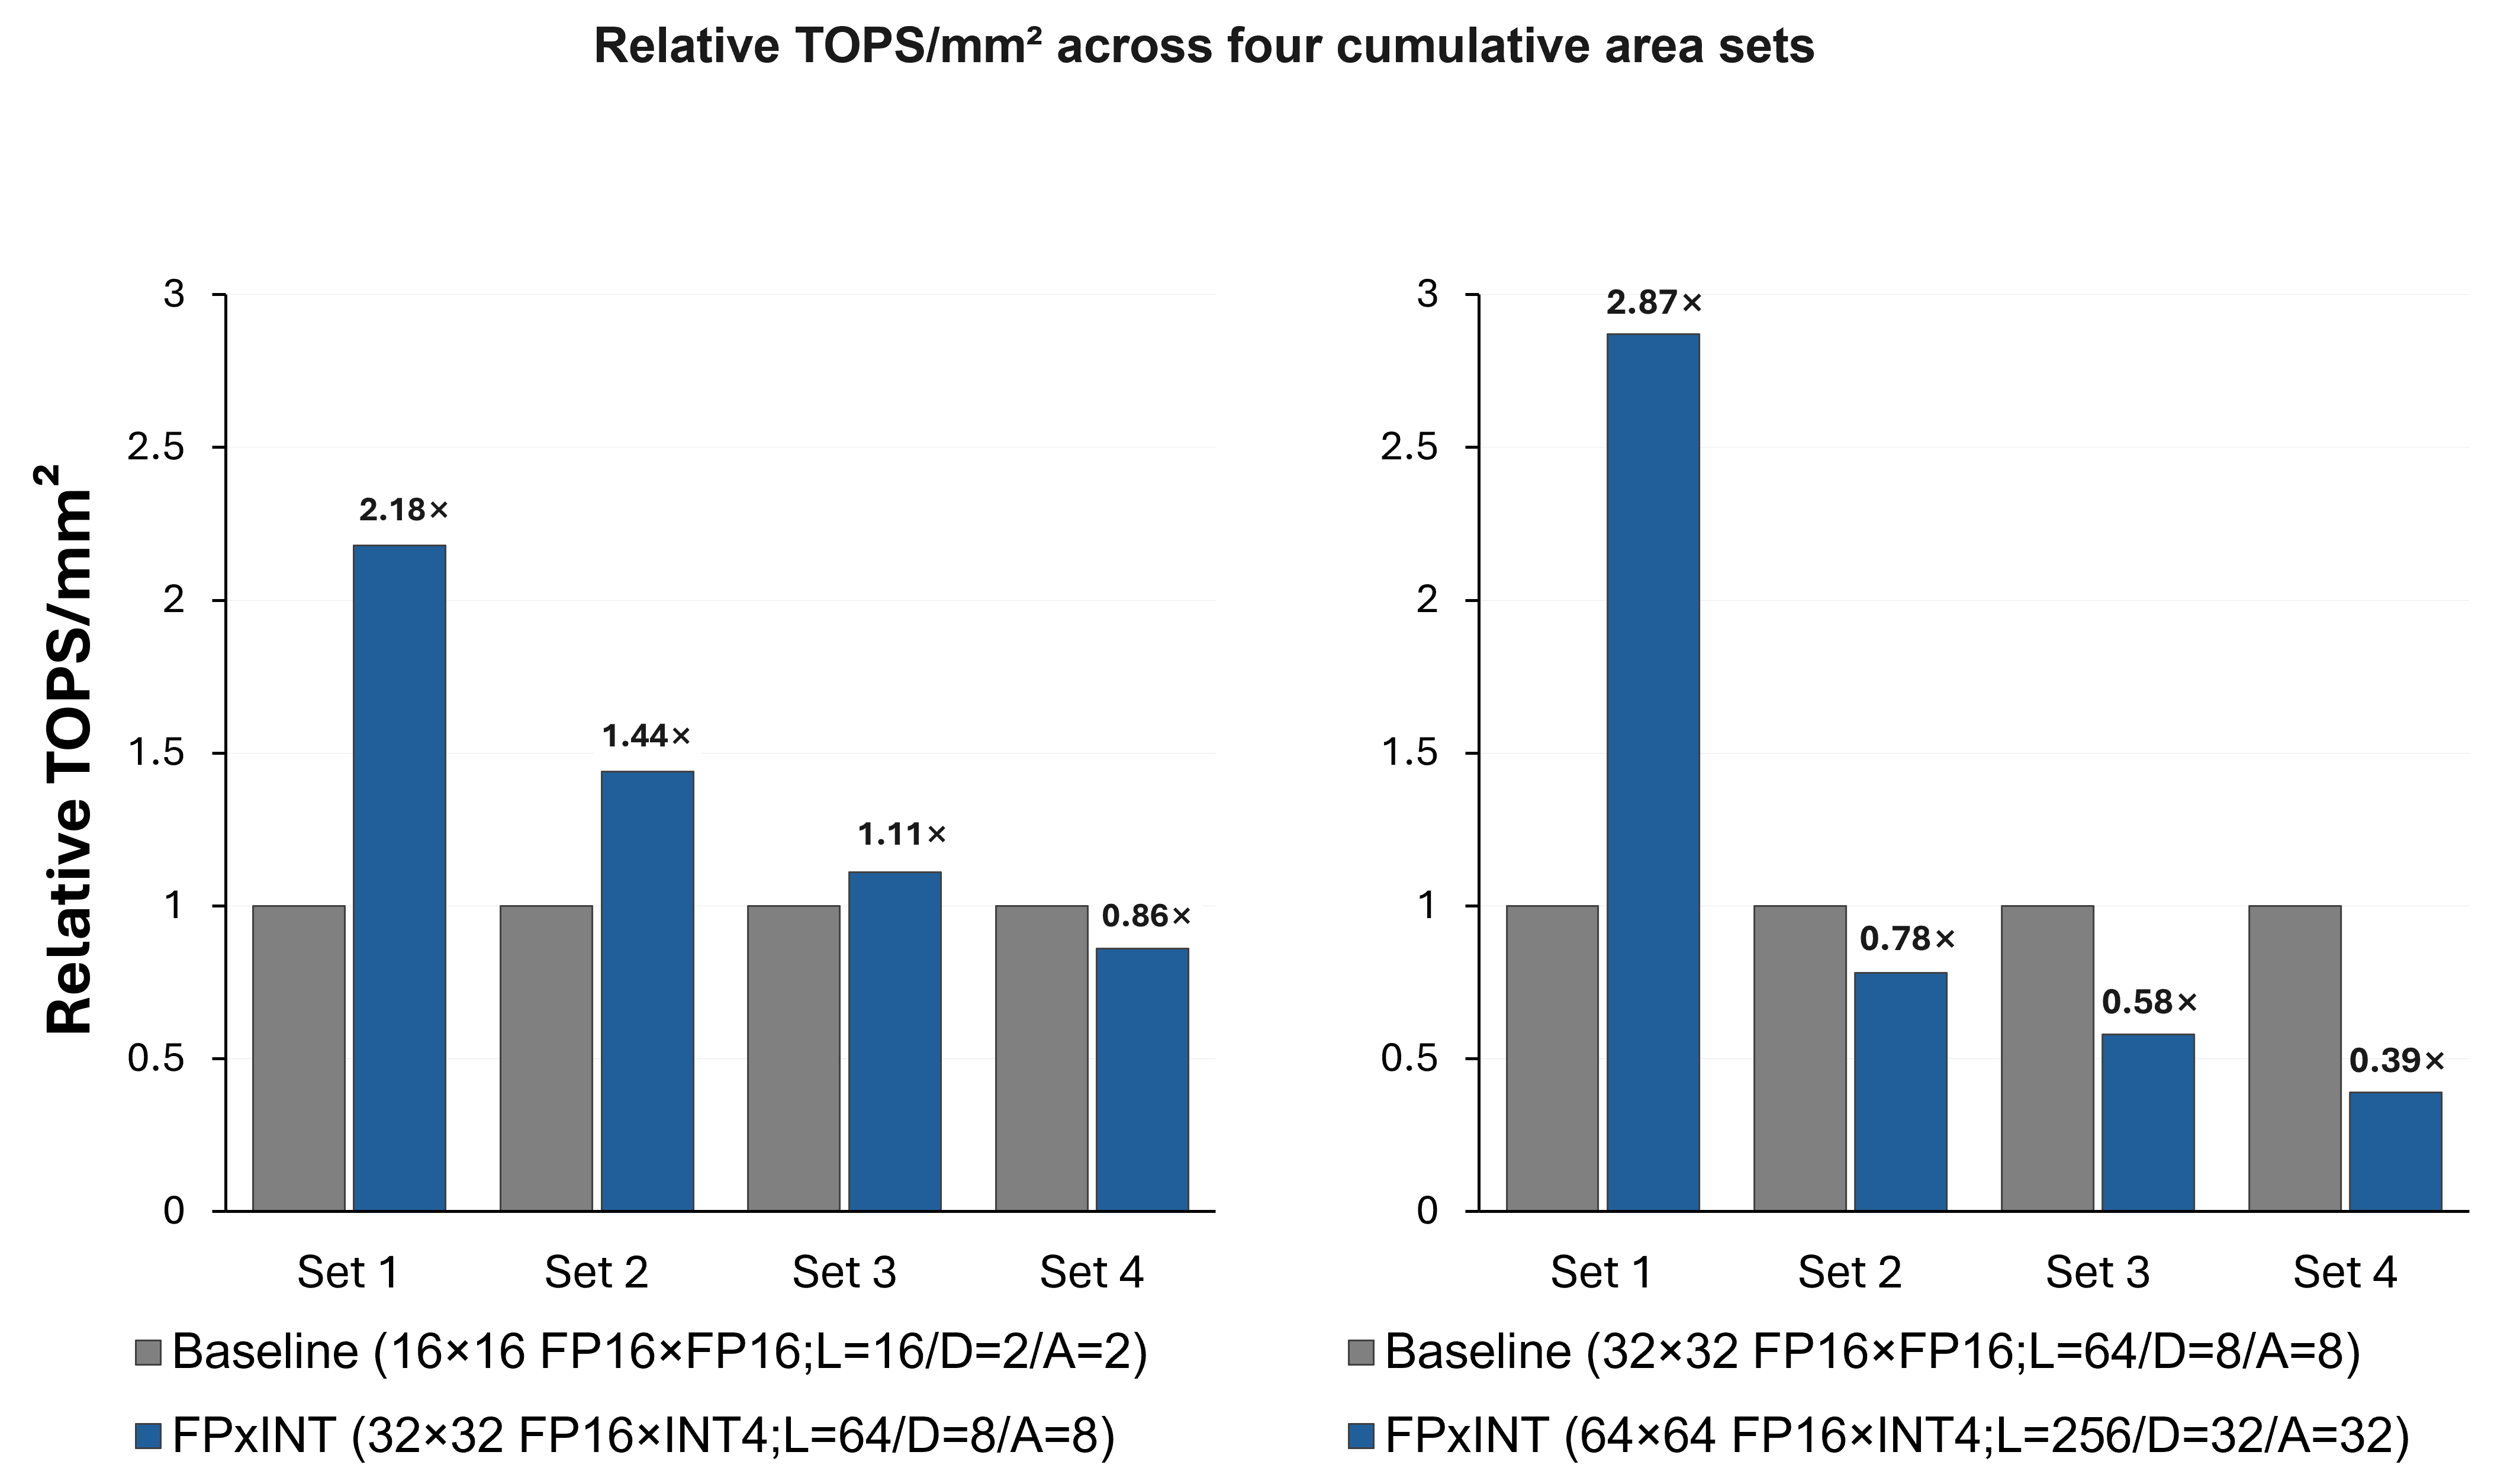
\includegraphics[width=0.98\linewidth]{figures/xbar_overhead_value.png}
%    \caption{Relative TOPS/mm$^2$ of FP$\times$FP and \fpint{} GEMM arrays as memory system area is progressively included. Bars are normalized to the FP$\times$FP baseline within each set, and absolute areas are shown inside the bars. Set~1 includes only the placed and routed MXU. Set~2 adds the crossbar and its control logic. Set~3 also includes the SRAM peripheral overhead caused by the increased bank count. Set~4 uses the placed and routed area of the full memory system. The intrinsic SRAM cell area is excluded, while SRAM peripheral overhead is charged only to the \fpint{} design. $L$, $D$, and $A$ denote the numbers of local memory banks, data cache banks, and AXI ports, respectively. Their values are chosen to match the ridge point of the GEMV roofline.}
%    \label{fig:xbar_overhead}
%\end{figure}
\begin{figure}[t]
    \centering
    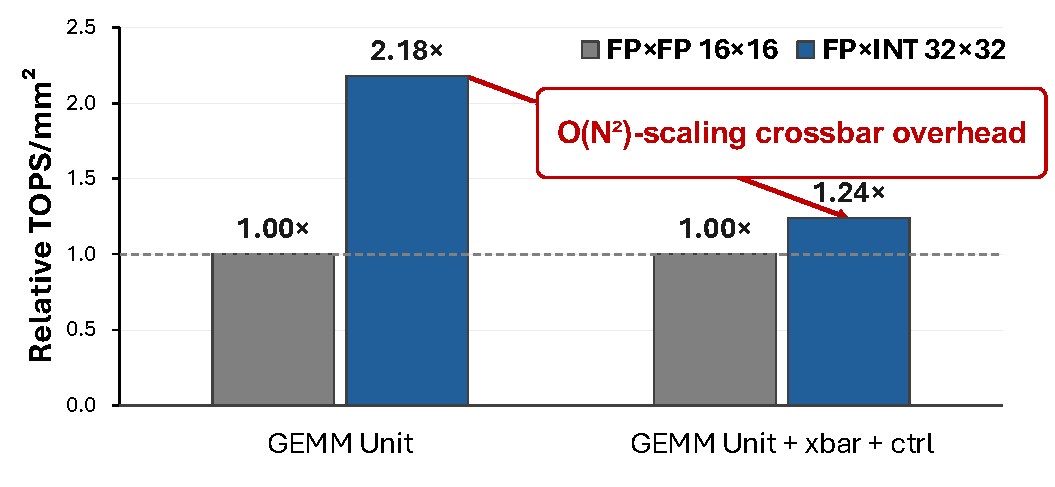
\includegraphics[width=0.85\linewidth]{figures/fig5.pdf}
    \caption{Relative TOPS/mm² of FP×FP and FP–INT GEMM units as crossbar and memory-system areas are progressively included. It shows diminishing relative TOPS/mm² gains of FP–INT over FP×FP with MXU and crossbar bandwidth scaling. To match the ridge point of the GEMV roofline, the local-memory bank count is increased from 16 to 64, the D-cache bank count from 2 to 8, and the number of HBM access ports from 2 to 8.}
    \label{fig:xbar_overhead}
\end{figure}
\fi
%Jae-Joon
\end{comment}

%Jae-Joon
\section{Overview of The Proposed \ours{} System}
\label{sec:overview}

\begin{figure*}[t]
    \centering
    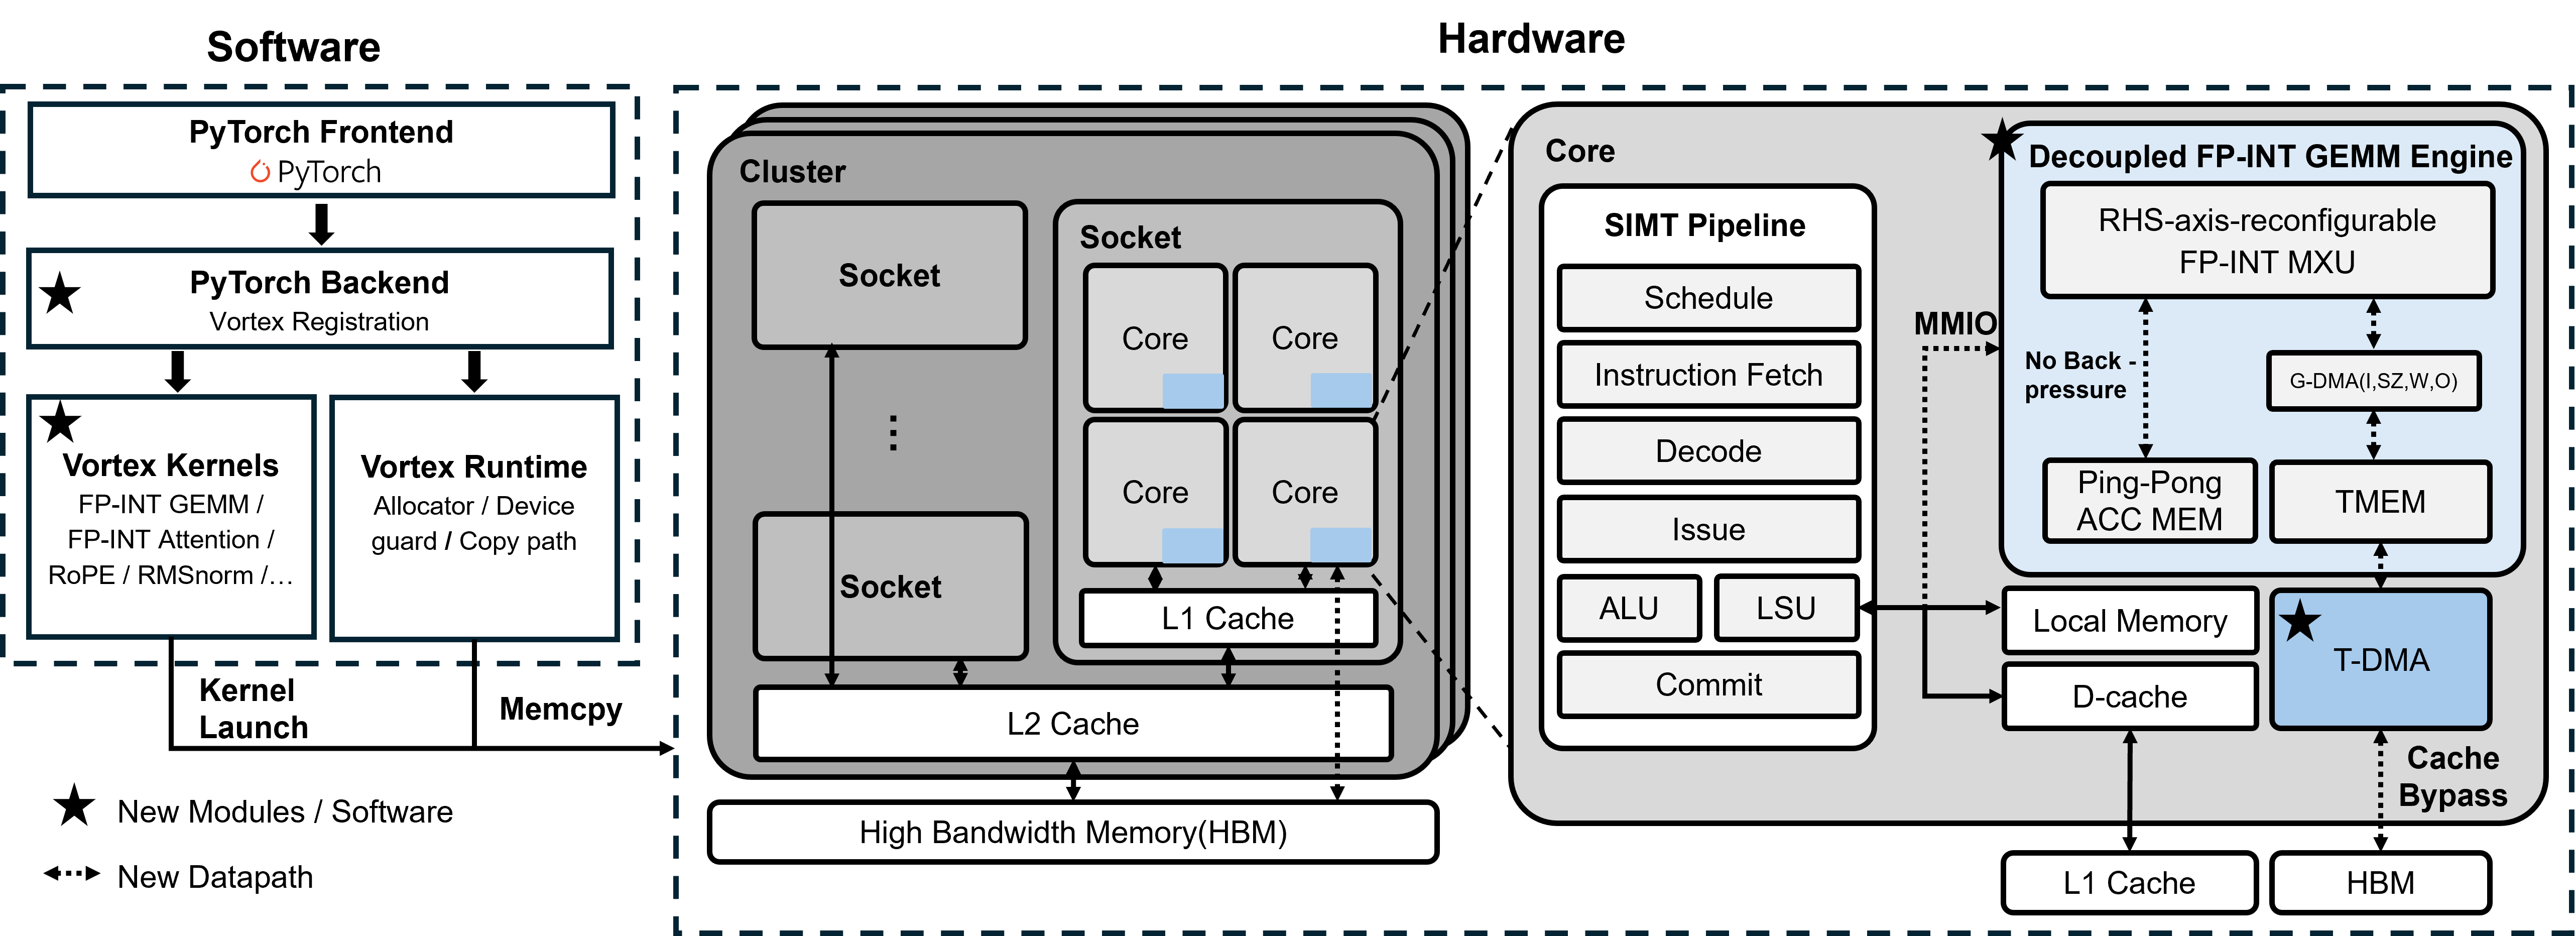
\includegraphics[width=0.95\linewidth]{figures/top_diagram.png}
    \caption{Overview of the \ours{} hardware/software system and its end-to-end execution flow.}
    \label{fig:overview}
\end{figure*}


\subsection{Overall Architecture}
\ours{} is an end-to-end hardware/software system for LLM inference with quantized weights and KV cache. It builds on 
Vortex~\cite{tine2021vortex}, an open-source GPGPU, and integrates a native \fpint{} GEMM engine with a dedicated tensor-memory subsystem and the runtime and kernel support required to use it. 
Figure~\ref{fig:overview} shows the high-level organization of \ours{}.
LLM inference contains control flow and vector operations, including normalization, activation functions, softmax, elementwise operations, quantization, and layout manipulation, in addition to GEMMs. Although these vector operations account for a relatively small fraction of the total arithmetic work, offloading them to a host CPU would incur frequent synchronization and data-transfer overheads. The orignal Vortex SIMT pipeline therefore remains responsible for control flow, vector kernels, kernel launch, and synchronization, while a decoupled \fpint{} GEMM engine executes the linear and attention GEMMs through memory-mapped IO (MMIO)-issued descriptors.

To make the end-to-end FP-INT LLM inference system more effective, we introduce several design features as follows.

\subsection{Quantization-Direction Aware Reconfigurable Dataflow}
The \fpint{} GEMMs in a \wkv{}-quantized model differ in how quantization metadata is organized for the INT operand and whether that operand is presented to the MXU in standard or transposed form. \ours{} captures these differences using two independent, per-GEMM configuration attributes: (1) quantization direction (\qcol{} or \qrow{}), (2) Loading choice for quantized operand (Standard or Transposed).
%The quantization direction selects either \qcol{} or \qrow{} metadata handling, while the load orientation selects standard or transposed loading of the INT operand. Linear projections, FFN layers, and $PV$ use the standard orientation, whereas $QK^T$ consumes K in transposed orientation. As summarized in Table~\ref{tab:kv_quant_direction}, token-wise and channel-wise quantization of the original K and V tensors map differently to \qcol{} and \qrow{} depending on the operation and load orientation. 
By configuring these two attributes independently, the same physical \fpint{} GEMM engine in FINISH can support the required execution modes across linear and attention layers with minimal hardware overhead. Section~\ref{sec:fpint-gemm-engine} details the corresponding datapaths and execution mechanisms.

\subsection{Tensor Memory System and Data Path for Improved GEMM Engine Utilization}
Naively scaling a conventional crossbar-based memory system with a denser \fpint{} MXU can diminish its array-level TOPS/mm$^2$ advantage.
To efficiently feed the larger number of FP-INT MACs over conventional FP-FP MACs, FINISH employs dedicated memory (TMEM) and datapath for Tensor data, which separates regular tensor traffic from general-purpose SIMT load/store traffic.
The dedicated tensor path allow \ours{} to increase \fpint{} compute density without proportionally scaling the register-file, cache, and local-memory interconnects. Detailed discussions are given in Section~\ref{sec:memory-system}.
%To efficiently feed the larger number of FP-INT MACs over conventional FP-FP MACs, FINISH employs dedicated memory for Tensor data (TMEM). Tensor operands are transferred among HBM pseudo-channels, TMEM, and the GEMM engine through a cache-bypassing, high-bandwidth tensor path. This path separates regular tensor traffic from general-purpose SIMT load/store traffic. Dedicated accumulator memory keeps wide partial sums off the input and weight paths, preventing accumulation traffic from interfering with operand delivery. Together, the decoupled GEMM engine and the dedicated tensor path allow \ours{} to increase \fpint{} compute density without proportionally scaling the register-file, cache, and local-memory interconnects. Detailed discussions are given in Section~\ref{sec:memory-system}.

\subsection{Hardware Constraint-Aware Data Mapping and Allocation}
The dedicated TMEM and tensor datapath with simplified connectivity trades general address flexibility for lower hardware overhead. 
Because GEMM tensors exhibit regular tiled access patterns, \ours{} satisfies these constraints through alignment-aware HBM allocation and compatible tensor layouts. This design scales the available tensor-memory bandwidth to $8\times$ that of the baseline with only an approximately 4\% increase in total area. Detailed discussions are given in Section~\ref{sec:runtime-section}.

\subsection{Hardware-Generated GEMM command stream}
%\textbf{Hardware-generated GEMM command stream.}
A large \fpint{} MXU needs command bandwidth as well as operand bandwidth. In our initial design, a kernel built tile-level commands through bit manipulation and enqueued them with store instructions, but on Vortex this scalar command stream became the launch bottleneck. 
FINISH instead has the kernel write the matrix dimensions, tile dimensions, tensor, accumulator, scale, and zero-point base addresses, quantization direction (qdir), and load direction to MMIO registers, and then initiate execution by writing 1 to the start bit in the MMIO registers.
A micro-op FSM inside the GEMM engine expands the descriptor into DMA, load direction of the quantized input, MXU step, accumulator update, and completion signaling. The SIMT pipeline therefore handles compact descriptor setup and synchronization, while hardware generates the repetitive GEMM command stream.
%Jae-Joon


\begin{comment}
\section{\ours{} Design Overview}

\begin{figure*}[t]
    \centering
    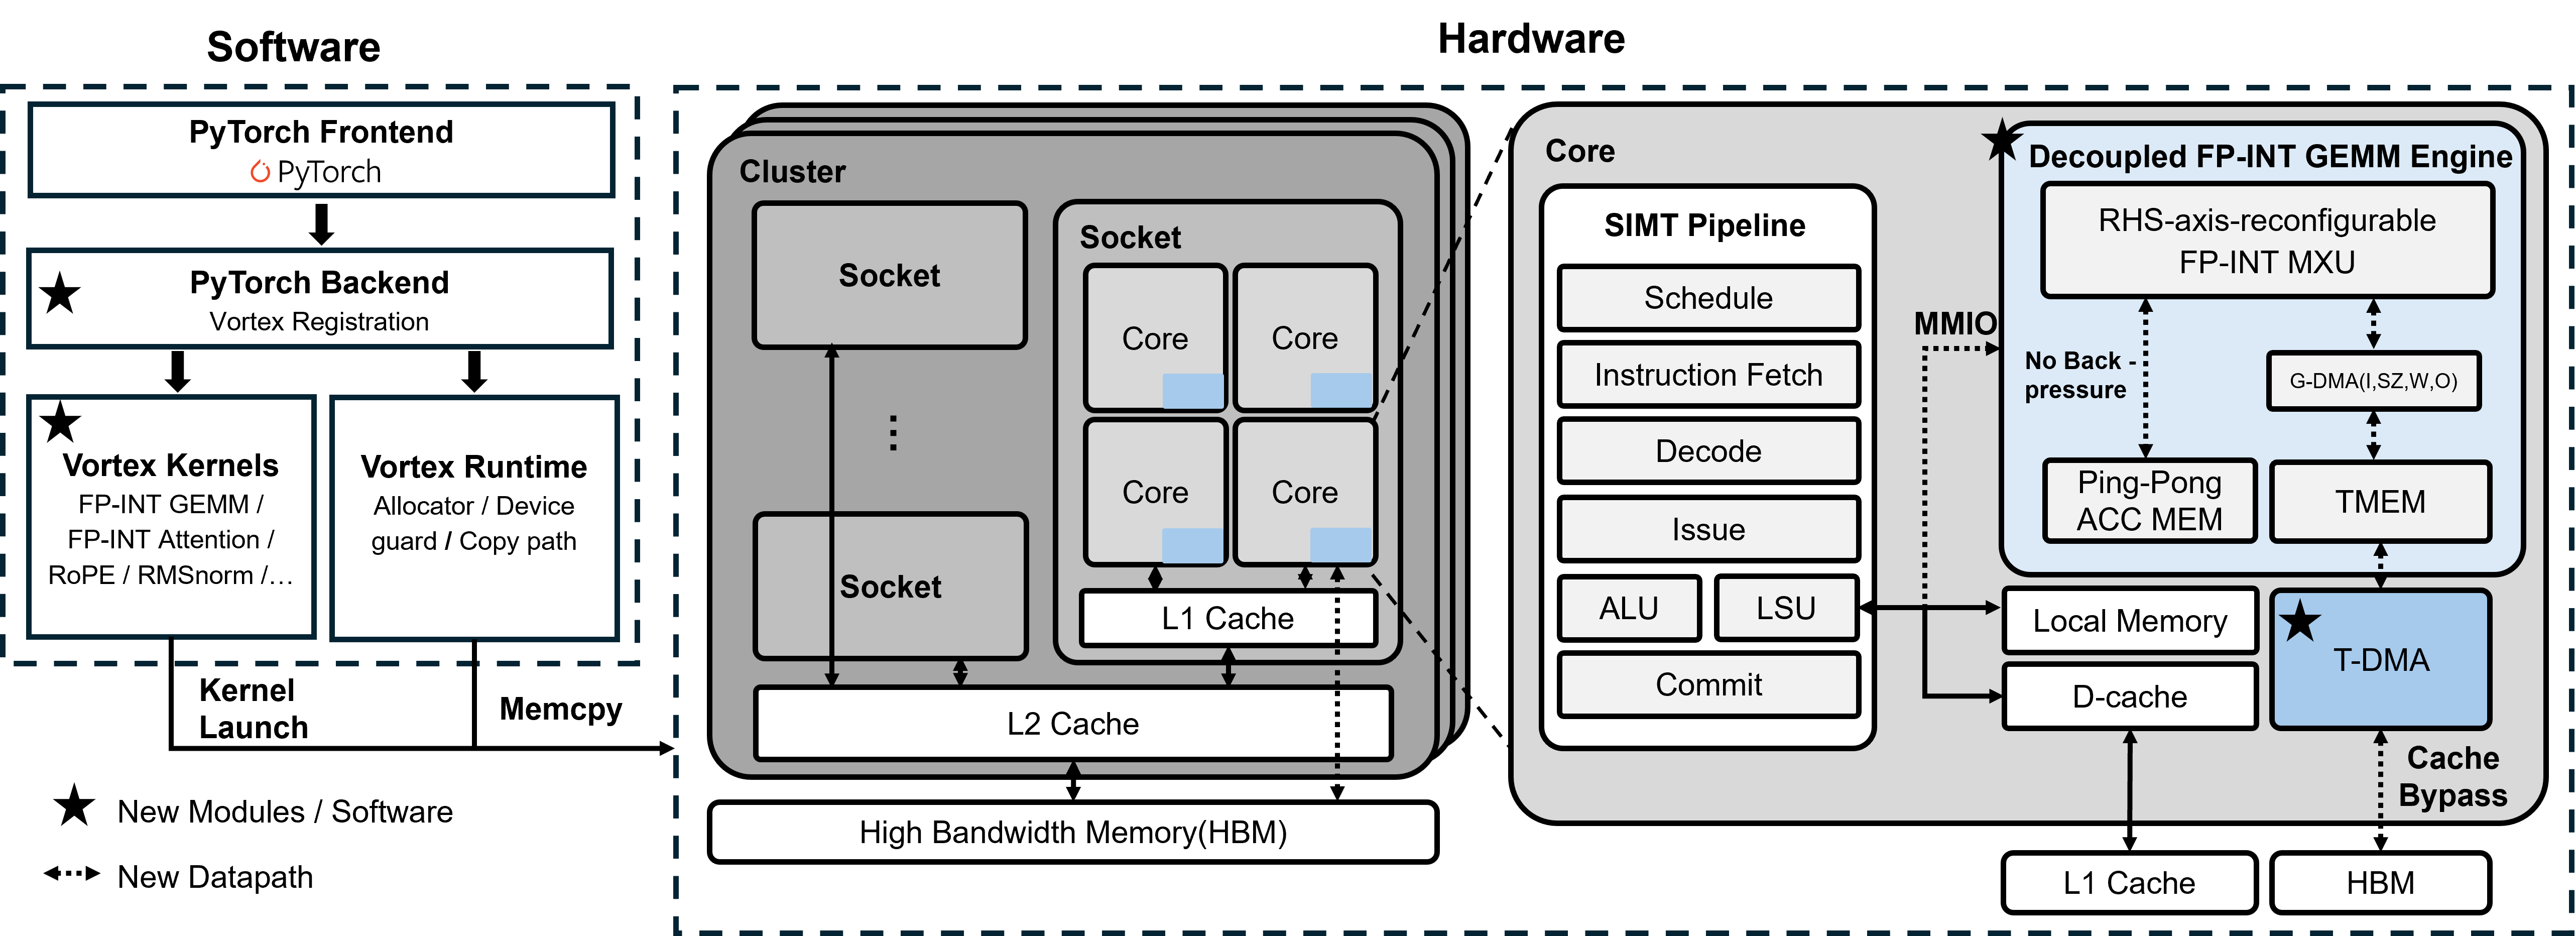
\includegraphics[width=0.95\linewidth]{figures/top_diagram.png}
    \caption{Overview of the proposed hardware/software system.}
    \label{fig:overview}
\end{figure*}

\ours{} is built on Vortex~\cite{tine2021vortex}, an open source GPGPU, and accelerates WKV quantized models by integrating an \fpint{} GEMM engine with an efficient memory subsystem and the runtime and kernel support required to use it.
Figure~\ref{fig:overview} shows the high-level organization of \ours{}.
The original Vortex SIMT pipeline remains responsible for control flow, vector operations, kernel launch, and synchronization, while a decoupled \fpint{} GEMM engine executes the linear and attention GEMMs through MMIO-issued descriptors.
%Tensor operands move between HBM pseudo channels, tensor memory, and the GEMM engine through a cache bypassed direct tensor path. 
Tensor operands are transferred among HBM pseudo-channels, tensor memory, and the GEMM engine through a cache-bypassing, high-bandwidth tensor data path equipped with DMA units that support aligned access across multiple channels.
The runtime and kernels manage layout, alignment, and synchronization so that this restricted path can be used efficiently.
To make this system effective end-to-end, we make several design decisions.

\textbf{Retaining the Vortex SIMT pipeline.}
An LLM contains a variety of vector operations in addition to GEMM. Even though these vector operations carry a small fraction of the total work, falling back to a CPU for them would incur a large overhead. We therefore keep the SIMT pipeline to preserve programmability and generality.

% \paragraph{The \fpint{} GEMM engine must support every combination of quantization direction and load direction for the right hand side operand.}
\textbf{Reconfigurable quantization and load directions for the right hand side.}
The \fpint{} GEMMs that appear repeatedly in a \wkv{} quantized model vary along two hardware axes for the RHS operand of the MXU. The RHS quantization direction is either \qcol{} or \qrow{}. The RHS load direction determines whether the operand is consumed in its standard or transposed orientation. In QK$^T$, the RHS must be consumed in transposed form, whereas in PV, the linear projections, and the FFN, the RHS is not transposed. Table~\ref{tab:kv_quant_direction} describes the token-wise and channel-wise quantization directions of the original K and V tensors. Their mapping to \qcol{} or \qrow{} depends on the operation and the RHS load direction. The \fpint{} GEMM engine must therefore support all four hardware execution patterns in a reconfigurable manner.

% \paragraph{We decouple the GEMM engine from SIMT and use dedicated tensor memory and accumulator memory.}
\textbf{Decoupled GEMM engine with a dedicated tensor path.}
Virgo previously demonstrated that a matrix unit can be physically disaggregated from the SIMT cores and placed at the GPU cluster level. This organization bypasses the capacity and bandwidth limitations of the SIMT register file and also supports separate accumulator memory~\cite{virgo}. We build on this established organization for a denser \fpint{} engine and focus on supplying the data bandwidth needed to keep it utilized. Virgo supplies matrix operands through cluster shared memory. For our \fpint{} engine, scaling the shared memory crossbar to the required bandwidth would be costly, and SIMT load and store traffic could interfere with tensor traffic. \ours{} therefore uses dedicated tensor memory and places accumulator memory inside the GEMM engine. The accumulator memory keeps wider partial sums off the input and weight path and enables a conflict free ping pong schedule on two single port SRAMs, so the GEMM pipeline can run without back pressure.

% \paragraph{The GEMM command stream is generated by a hardware micro-op FSM, not by a software queue.}
\textbf{Hardware-generated GEMM command stream.}
A large \fpint{} MXU needs command bandwidth as well as operand bandwidth. In our initial design, a kernel built tile-level commands through bit manipulation and enqueued them with store instructions, but on Vortex this scalar command stream became the launch bottleneck. 
%\ours{} instead has the kernel write the matrix shape, tile shapes, tensor/accumulator/scale/zero-point base addresses, quantization direction (\texttt{qdir}), and load direction into MMIO registers, then submit the request through a doorbell.
FINISH instead has the kernel write the matrix dimensions, tile dimensions, tensor, accumulator, scale, and zero-point base addresses, quantization direction (qdir), and load direction to MMIO registers, and then initiate execution by writing 1 to the start bit in the MMIO registers.
A micro-op FSM inside the GEMM engine expands the descriptor into DMA, RHS load, MXU step, accumulator update, and completion signaling. The SIMT pipeline therefore handles compact descriptor setup and synchronization, while hardware generates the repetitive GEMM command stream.

% \paragraph{Rather than scaling the memory subsystem with a complex crossbar, we scale it at low cost with a simple interconnect fabric and handle the resulting constraints in the software stack.}
\textbf{Low-Cost, Restricted Interconnect with Software-Handled Constraints.}
Naively scaling full-crossbar memory components can eliminate the TOPS/mm$^2$ gain of the \fpint{} array. At the HBM--TMEM boundary, \ours{} replaces a full crossbar with a fixed 1:1 or interleaved fabric. At the TMEM--MXU boundary, four fixed 64\,B GEMM ports select among the TMEM banks through restricted wide-word mux/demux paths. Tensor traffic is carried on a cache-bypassed DMA path. When a vector stage is fused before GEMM, it issues a fence after producing the GEMM inputs. When a vector stage follows GEMM, it polls a read-only MMIO register that reports completed result tiles. The tradeoff is a set of boundary-specific mapping and alignment constraints that the software stack must satisfy.
%Because GEMM traffic is regular, constraint-aware HBM allocation and tensor layout can satisfy these constraints while scaling memory bandwidth by $8\times$ with only about a 4\% increase in total area.
Because GEMM traffic exhibits regular access patterns, constraint-aware HBM allocation and tensor layouts can satisfy these requirements while scaling memory bandwidth to $8\times$ the baseline, with only an approximately 4\% increase in total area.
\end{comment}

\section[Native FP-INT Attention Support]{Native \texorpdfstring{\fpint{}}{FP-INT} Attention Support}

As discussed in Section~\ref{sec:sys_gap}, native \fpint{} attention requires more than an MXU that multiplies one FP operand by one INT operand. The key issue is whether the quantization metadata changes along the GEMM reduction direction. If one scale and zero point are shared across the values being reduced, the MXU can first compute the INT dot product and apply dequantization afterward. This is the common case in GEMMs in linear layers, where metadata is fixed by output channel or group. 
%In KV-cache quantization, however, QK$^T$ and PV map token and channel axes to different GEMM directions. 
In KV-cache quantization, however, the key and value caches can each be quantized along either the token or channel dimension, with the selected quantization axes varying across frameworks.
%A scheme that keeps metadata outside the reduction direction in one attention GEMM can place different scales along the reduction direction in the other. 
In that case, each product must be dequantized before accumulation, so a conventional \fpint{} MXU needs per-term FP multiplication and FP reduction or falls back to the FP attention path.

To address this, we propose a \fpint{} MXU that independently reconfigures the RHS quantization direction between \qcol{} and \qrow{} and separately configures the RHS load direction. The \texttt{qdir} field selects where the \fpint{} GEMM applies the scale and the zero point. In the following, $A$ is the FP input operand, $B^{int}$ is the INT RHS operand, $G_K$ and $G_N$ are the quantization group sizes along the reduction and output dimensions, $g(k)=\lfloor k/G_K \rfloor$, and $h(n)=\lfloor n/G_N \rfloor$.

The same prealigner is shared by \qcol{} and \qrow{}. We follow the numerical accuracy preserving prealignment scheme of FIGNA~\cite{figna} and represent each FP16 input using a 31 bit signed aligned mantissa before integer multiplication and reduction. The subsequent integer accumulation and conversion back to FP also follow FIGNA.

In \qcol{}, the scale and the zero point are bound to the reduction group and the output column. Within a group, $S^{\mathrm{COL}}_{g,n}$ and $Z^{\mathrm{COL}}_{g,n}$ are invariant in the reduction index $k$, so output scaling can be deferred to the end of the dot product:
\begin{align}
    C^{\mathrm{COL}}_{m,n}
    &=
    \sum_g S^{\mathrm{COL}}_{g,n}
    \left(
        \sum_{k \in \mathcal{K}_g} A_{m,k} B^{int}_{k,n}
        -
        Z^{\mathrm{COL}}_{g,n} \sum_{k \in \mathcal{K}_g} A_{m,k}
    \right) .
    \label{eq:qcol-fpint}
\end{align}
Figure~\ref{fig:fpint-gemm-unit} shows how this \qcol{} computation is implemented. The Conditional Input Scaling Unit~\blackcircletext{1} selects the unscaled activation and forwards it to the prealigner. After prealignment, the Reconfigurable Zero-Point Correction Unit~\blackcircletext{2} and the Transposable MXU~\blackcircletext{3} operate in parallel. The former reduces the aligned activations and then multiplies the result by $-Z^{\mathrm{COL}}_{g,n}$, while the latter computes the main product $\sum \hat{A} B^{int}$. The FP Output Reconstructor~\blackcircletext{4} merges the correction and main-product paths, converts the result back to FP, and applies $S^{\mathrm{COL}}_{g,n}$. This dataflow is possible because the scale remains stationary along the output lane.

In \qrow{}, by contrast, the scale and the zero point are bound to the reduction index and the output group. The direct \qrow{} computation is
\begin{align}
    C^{\mathrm{ROW}}_{m,n}
    &=
    \sum_k A_{m,k}
    \left(
        S^{\mathrm{ROW}}_{k,h(n)} \cdot
        (B^{int}_{k,n} - Z^{\mathrm{ROW}}_{k,h(n)})
    \right) .
    \label{eq:qrow-direct}
\end{align}
Because $S^{\mathrm{ROW}}_{k,h(n)}$ changes with $k$, it cannot be factored out of the reduction, and \qcol{} scaling after accumulation is no longer valid. Likewise, the $k$-dependent zero point prevents a single correction after first reducing the activations. A direct datapath would therefore need to dequantize each term before accumulation, which is inefficient.

The \qrow{} datapath does not eliminate the scale multiplication required for each reduction term.
Instead, the Conditional Input Scaling Unit~\blackcircletext{1} moves this multiplication from RHS dequantization to the FP input before prealignment.
Define $\bar{A}^{(h)}_{m,k}=A_{m,k}S^{\mathrm{ROW}}_{k,h(n)}$. The \qrow{} computation then becomes
\begin{align}
    C^{\mathrm{ROW}}_{m,n}
    &=
    \sum_k \bar{A}^{(h)}_{m,k} B^{int}_{k,n}
    -
    \sum_k \bar{A}^{(h)}_{m,k} Z^{\mathrm{ROW}}_{k,h(n)},
    \label{eq:qrow-fpint}
\end{align}
The scale is now absorbed into $\bar{A}$ before the prealigner converts the FP vector into the aligned integer representation used by the MXU.
The downstream datapath therefore does not consume scale metadata that varies along the reduction dimension.
Equivalently, every reduction term after prealignment has an effective scale of one.
This does not mean that the scale metadata is rewritten to one. It means that the scale has already been applied to the FP input and no additional scale operation remains in the reduction path.
The main product and zero point correction can therefore use integer reduction.
The remaining zero point term is handled by the correction path selected by \texttt{qdir} as described below.
Although $S^{\mathrm{ROW}}_{k,h(n)}$ is indexed by the output group, $h(n)$ is invariant within an MXU tile.
Our 32$\times$32 MXU supports quantization group sizes of 32, 64, and 128 along the output dimension.
When a GEMM dimension does not align with a quantization group boundary, the kernel pads it to the next boundary, so a 32 column MXU tile never spans two output groups.
Consequently, all columns in an MXU tile use the same scale vector.
The input scaler in component~\blackcircletext{1} applies this scale vector before prealignment, and the resulting activation vector is reused by all 32 MXU columns.
For our 32$\times$32 MXU, component~\blackcircletext{1} contains 32 FP multipliers rather than 1024 per-PE multipliers.
This organization requires neither a separate scaled activation for each column nor activation replay across columns.
% ---------------------------------------------------------------------
% The Reconfigurable Zero-Point Correction Unit~\blackcircletext{2} implements zero-point correction in an order selected by \texttt{qdir}. We denote the prealigner output as $\hat{A}$ in \qcol{} and as $\hat{\bar{A}}$ in \qrow{}. For notational simplicity, the exponent and shift corrections are absorbed into these representations. In \qcol{}, the zero point varies only across columns within a group, so the activation sum is formed first and then multiplied by the column-specific zero point:
% \begin{align}
%     P^{\mathrm{COL}}_{m,n} &= \sum_{k \in \mathcal{T}} \hat{A}_{m,k} B^{int}_{k,n}, \\
%     R^{\mathrm{COL}}_{m} &= \sum_{k \in \mathcal{T}} \hat{A}_{m,k}, \\
%     D^{\mathrm{COL}}_{m,n} &= (-Z^{\mathrm{COL}}_{g,n}) R^{\mathrm{COL}}_{m}, \\
%     I^{\mathrm{COL}}_{m,n} &= P^{\mathrm{COL}}_{m,n} + D^{\mathrm{COL}}_{m,n} .
%     \label{eq:qcol-correction}
% \end{align}
% Thus, the correction unit uses reduce-then-multiply in \qcol{}.

% In \qrow{}, the zero point differs per reduction lane, so summing the activations first would lose track of which zero point should be multiplied. We therefore form the lane-specific zero-point product first using $\hat{\bar{A}}$ and reduce those products afterwards:
% \begin{align}
%     P^{\mathrm{ROW}}_{m,n} &= \sum_{k \in \mathcal{T}} \hat{\bar{A}}^{(h)}_{m,k} B^{int}_{k,n}, \\
%     D^{\mathrm{ROW}}_{m,h} &= \sum_{k \in \mathcal{T}} (-Z^{\mathrm{ROW}}_{k,h}) \hat{\bar{A}}^{(h)}_{m,k}, \\
%     I^{\mathrm{ROW}}_{m,n} &= P^{\mathrm{ROW}}_{m,n} + D^{\mathrm{ROW}}_{m,h} .
%     \label{eq:qrow-correction}
% \end{align}
% The same reduce tree and zero-point multiplier are used in both directions, but component~\blackcircletext{2} changes the routing from reduce-then-multiply in \qcol{} to multiply-then-reduce in \qrow{}. This change preserves the per-$k$ zero-point correction required by \qrow{} while the Transposable MXU~\blackcircletext{3} computes the main product using the same INT RHS datapath. The FP Output Reconstructor~\blackcircletext{4} then merges $P$ and $D$, converts the result back to FP, and bypasses its output scaler in \qrow{} because component~\blackcircletext{1} has already applied the scale.
% ---------------------------------------------------------------------
% +++++++++++++++++++++++++++++++++++++++++++++++++++++++++++++++++++++
The Reconfigurable Zero-Point Correction Unit~\blackcircletext{2} forms the zero-point term in an order selected by the quantization direction. Let $\hat{A}$ and $\hat{\bar{A}}$ denote the prealigner outputs in \qcol{} and \qrow{} (absorbing exponent and shift corrections), and let $\mathcal{T}$ be the reduction lanes in one MXU step. In \qcol{}, the zero point is constant across $\mathcal{T}$, so the unit reduces the inputs first and multiplies once by the column zero point; in \qrow{}, it differs per lane, so the unit forms the lane-wise products first and reduces them afterward:
\begin{align}
    D^{\mathrm{COL}}_{m,n}
    &=
    \left(-Z^{\mathrm{COL}}_{g,n}\right)
    \sum_{k \in \mathcal{T}} \hat{A}_{m,k},
    \\
    D^{\mathrm{ROW}}_{m,h}
    &=
    \sum_{k \in \mathcal{T}}
    \left(-Z^{\mathrm{ROW}}_{k,h}\right)
    \hat{\bar{A}}^{(h)}_{m,k}.
\end{align}
The Transposable MXU~\blackcircletext{3} computes the main product $P_{m,n}=\sum_{k \in \mathcal{T}} \hat{A}_{m,k}B^{\mathrm{int}}_{k,n}$ on the same INT datapath, and the FP Output Reconstructor~\blackcircletext{4} adds $P$ and $D$ before converting back to FP. The same reduction tree and zero-point multiplier serve both modes; component~\blackcircletext{2} only reroutes from reduce-then-multiply (\qcol{}) to multiply-then-reduce (\qrow{}). The output scaler is enabled in \qcol{} and bypassed in \qrow{}, where component~\blackcircletext{1} has already applied the scale.
% +++++++++++++++++++++++++++++++++++++++++++++++++++++++++++++++++++++

Attention changes not only the quantization direction but also the logical orientation of the RHS. PV and linear GEMMs consume the RHS tile in the standard orientation, whereas QK$^T$ must feed the K tile to the MXU in transposed form. To support this, the Transposable MXU~\blackcircletext{3} duplicates the RHS load network so that the same array supports both row-wise and column-wise loading. The transpose is thus absorbed into a load-time configuration rather than handled by a separate memory-transform kernel. As shown in Figure~\ref{fig:fpint-gemm-unit}, \texttt{qdir} configures the scaling and zero-point-correction datapath, while the load direction independently determines how the RHS matrix is delivered to the weight input of the MXU. The upper-level architecture only needs to set \texttt{qdir} and load direction for each linear, QK$^T$, or PV kernel, while the physical \fpint{} MXU array is shared across all paths.

%The \texttt{DLY} block in Figure~\ref{fig:fpint-gemm-unit} is an FF-based delay element that matches the pipeline latency between the main product path and the correction path, both of which vary with \texttt{qdir} and load direction. 
The \texttt{DLY} block in Figure~\ref{fig:fpint-gemm-unit} is an FF-based delay element that matches the pipeline latency between the main product path and the correction path. 
With \texttt{DLY}, the \texttt{merger} and the accumulator stage receive cycle-aligned partial results. The \texttt{ACC MEM BANK} is dedicated storage for partial-sum accumulation. Instead of a true dual-port SRAM, it uses two single-port SRAM banks scheduled in a 1-cycle skewed ping-pong fashion: while one bank is read in a given cycle, the other is written, constraining the dataflow so that the two single-port banks behave as a logically dual-port accumulator bank.

\begin{figure}[t]
    \centering
    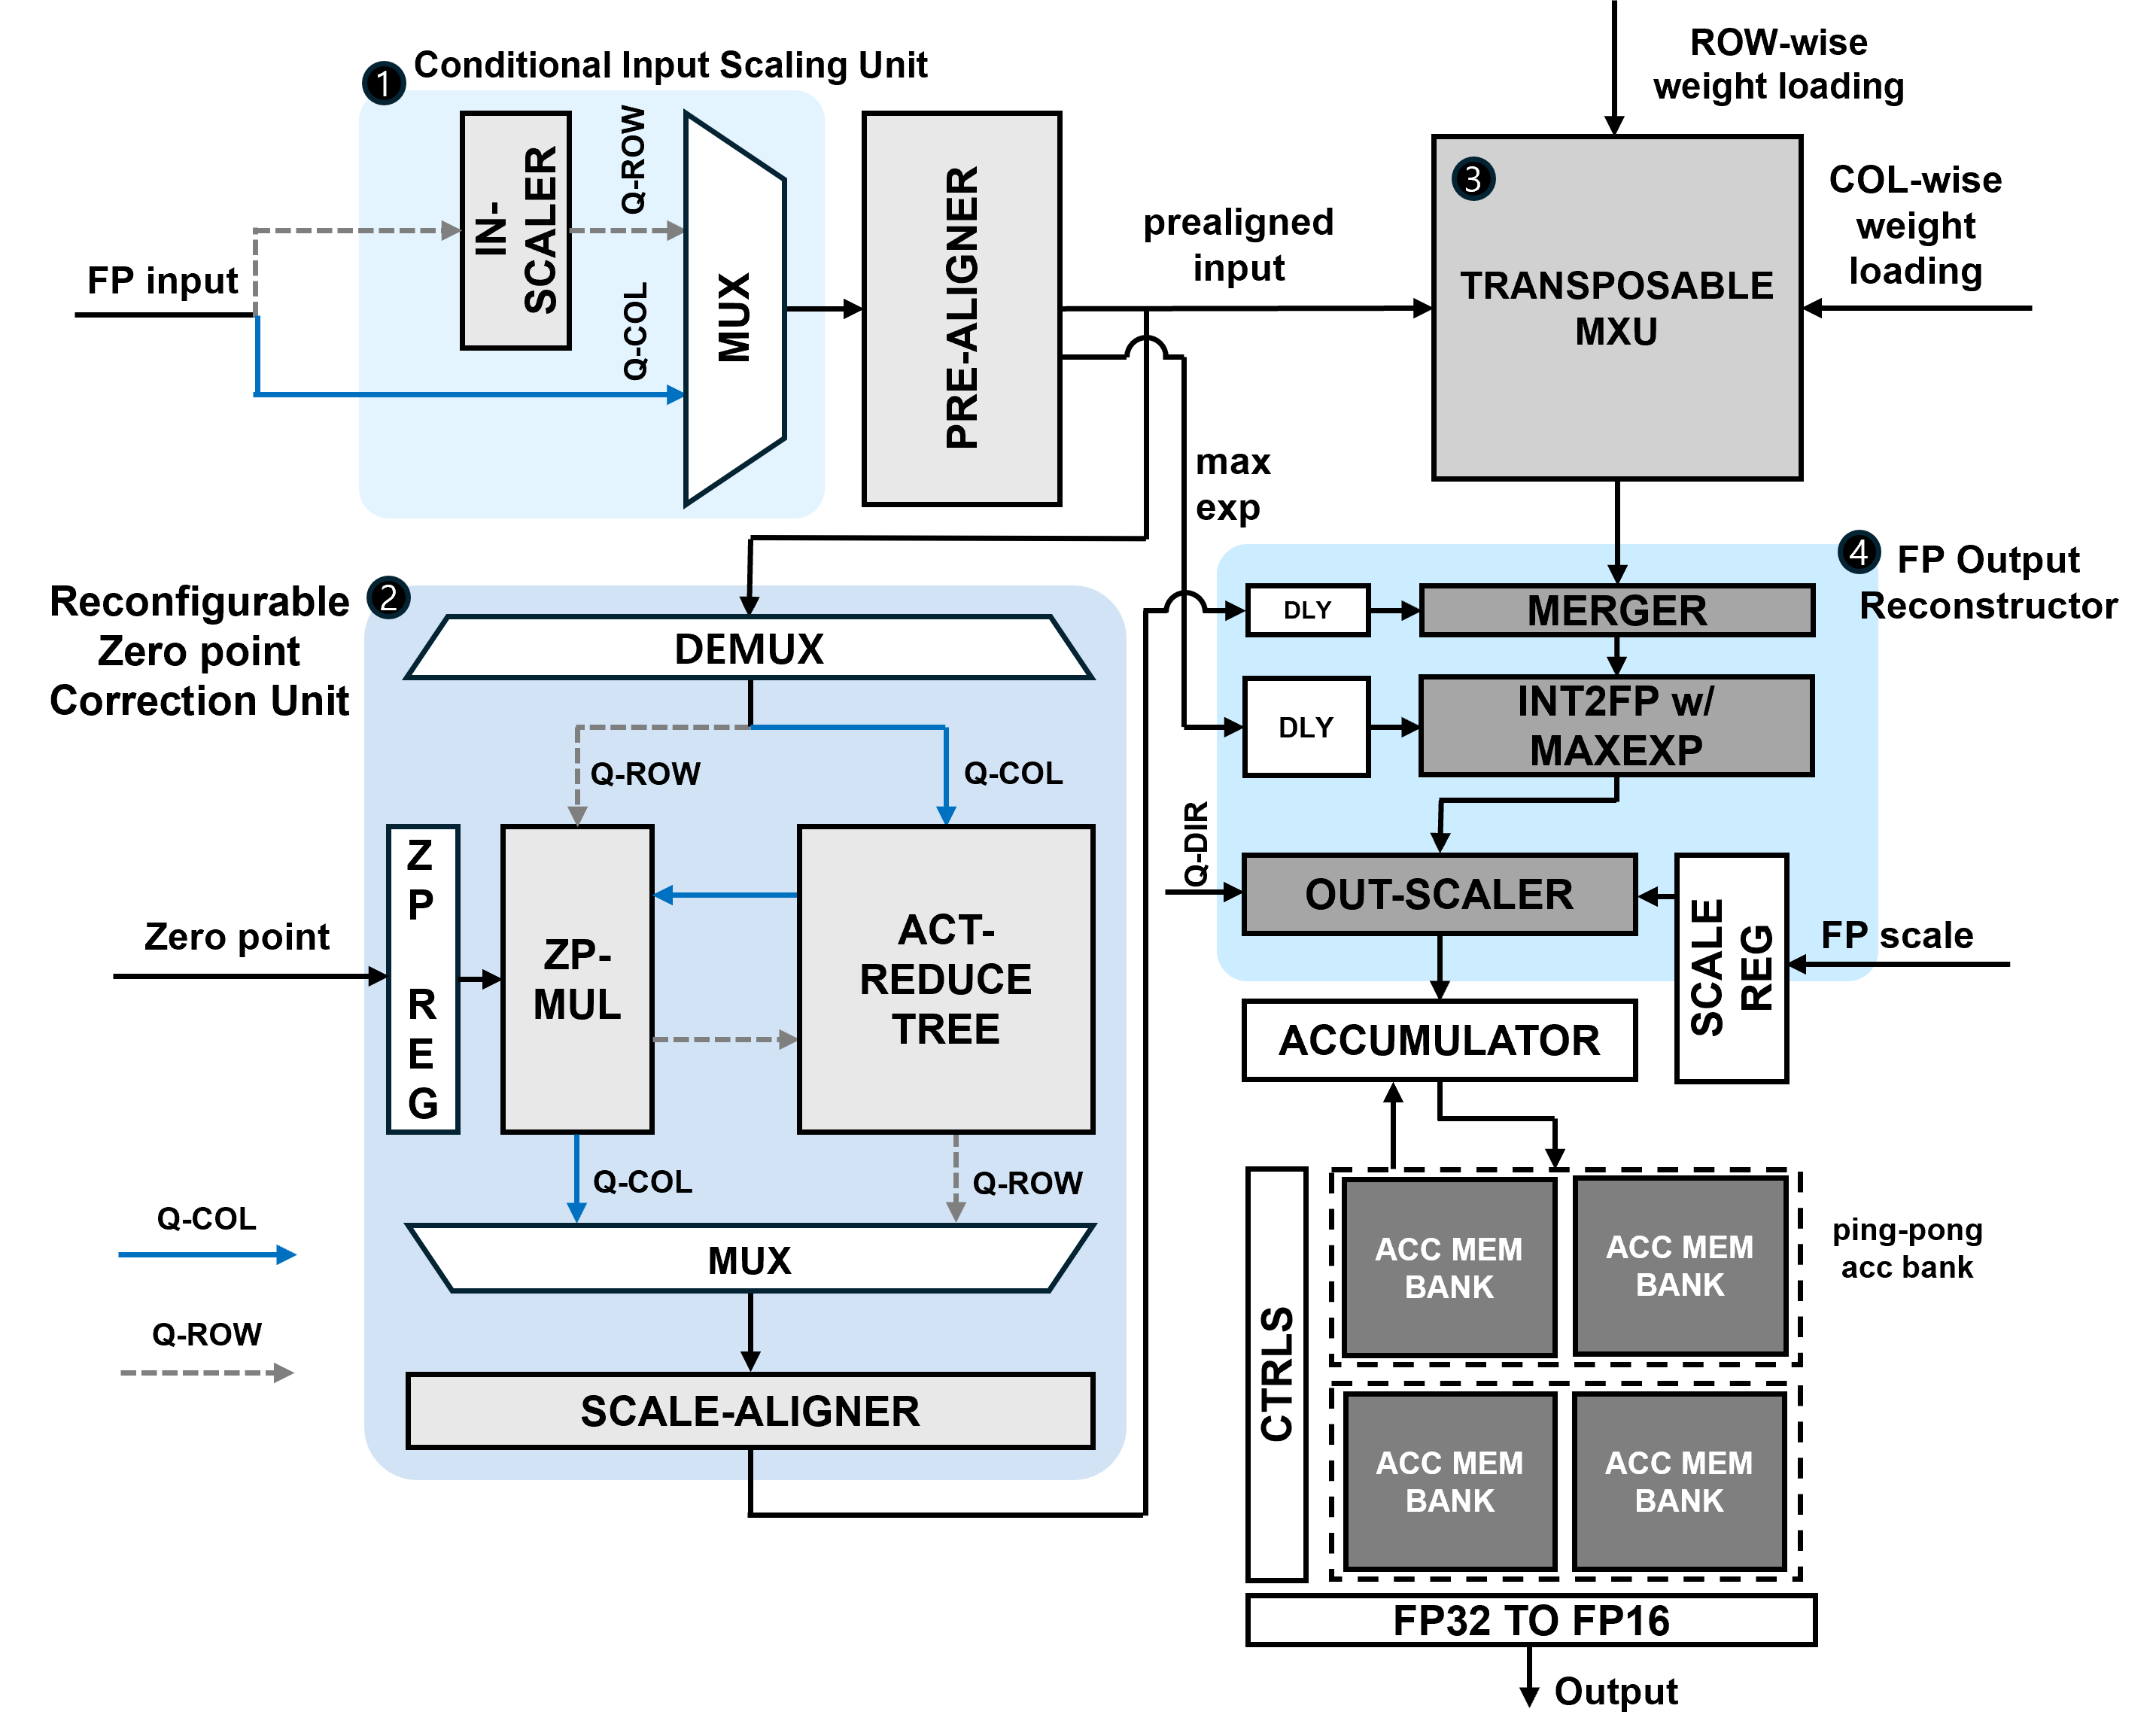
\includegraphics[width=0.92\linewidth]{figures/gemm_engine.png}
    \caption{RHS quantization direction reconfigurable \fpint{} GEMM unit with scale folding datapath and dual RHS load paths.}
    \label{fig:fpint-gemm-unit}
\end{figure}

The key effect is eliminating FP fallback in quantized attention. A linear-only \fpint{} design leaves attention as the long-context bottleneck, while the proposed MXU executes both QK$^T$ and PV as native \fpint{} GEMMs alongside the linear layers.

\section[Memory System for Sustained FP-INT Utilization]{Memory System for Sustained \texorpdfstring{\fpint{}}{FP-INT} Utilization}
\label{sec:memory-system}

An \fpint{} MXU can provide more MACs than an FP$\times$FP Tensor Core at smaller area and lower energy, but higher MAC density also raises operand-bandwidth demand. Supplying all operands through the register file, shared memory, and cache would make crossbar, arbitration, and routing costs grow with port and bank counts. The memory system of \ours{} therefore separates regular tensor traffic from the general-purpose memory path instead of simply attaching a larger array to the core.

\textbf{Partitioned On-Chip Tensor Storage.}
Local memory must remain flexible for conventional load/store, inter-thread communication, and scalar/vector kernels. GEMM operands, however, follow fixed tile shapes and access orders, so banked bandwidth matters more than arbitrary access. \ours{} partitions on-chip SRAM into general-purpose local memory, MXU-dedicated tensor memory, and accumulator memory. Tensor and accumulator memories scale bank count and data width under restricted access patterns, while local memory preserves the SIMT programming model. 
%Separating wider partial sums from input/weight traffic also removes read-modify-write interference and lets the deeply pipelined GEMM datapath avoid ready-signal back-pressure.
Storing wider partial sums in a dedicated ACC MEM, separate from input and weight traffic, removes read-modify-write interference and prevents ready-signal back-pressure from stalling the deeply pipelined GEMM datapath.

%\textbf{Interleaved-Connected Tensor Data Path.}
\textbf{Interleaved and Aligned Tensor Data Path.}
Connecting HBM pseudo-channels to tensor memory banks through a full crossbar is flexible, but its area and routing overhead grow super-linearly with bandwidth. \ours{} instead uses a fixed 1:1 or interleaved connection at the HBM--TMEM boundary. At the TMEM--MXU boundary, the GEMM engine exposes four fixed 64\,B vector ports for input, weight, scale/zero-point, and output traffic. Each read port is driven by an $N_{\mathrm{tmem}}$-to-1 bank-select multiplexer, while the output port uses the reverse demultiplexing path. Although these mux/demux paths can be viewed collectively as a restricted crossbar, they are simpler than the 8\,B-granular local-memory crossbar: the number and roles of the GEMM ports are fixed, and every request moves one aligned 64\,B TMEM bank word without byte-level steering, split accesses, or cross-bank realignment. Figure~\ref{fig:memory-system} illustrates these choices for 8 HBM pseudo-channels, 8 TMEM banks, and FP16 input precision. Here, $R_{\mathrm{MXU}}$ is the MXU row dimension, or the number of reduction lanes consumed per input slice.

The two boundaries impose different software-visible constraints. At the HBM--TMEM boundary, the HBM pseudo-channel and TMEM bank selected by the two addresses must be physically connected, and both DMA addresses must be aligned to the $DW$-byte transfer granularity. Consider two memory endpoints with $N_L$ and $N_S$ ports, where $N_L \geq N_S$. For a byte address $A_E$ at memory endpoint $E$, low-order interleaving selects
\begin{equation}
    b_E\left(A_E\right)
    =
    \left\lfloor
        \frac{A_E}{DW}
    \right\rfloor
    \bmod N_E .
    \label{eq:interleaved_endpoint_index}
\end{equation}
The fixed interconnect maps port $j$ of the larger endpoint to port $j \bmod N_S$ of the smaller endpoint. Consequently, a transfer between addresses $A_L$ and $A_S$ is possible only if
\begin{equation}
    b_S\left(A_S\right)
    =
    b_L\left(A_L\right)
    \bmod N_S .
    \label{eq:general_interleaved_constraint}
\end{equation}
Independently, the aligned-only DMA requires
\begin{equation}
    A_L \bmod DW
    =
    A_S \bmod DW
    =
    0 .
    \label{eq:aligned_dma_constraint}
\end{equation}
Equal endpoint counts give a 1:1 mapping; unequal counts give the deterministic interleaved mapping in Eq.~\ref{eq:general_interleaved_constraint}. For example, a 4-to-8 connection maps endpoint $i$ on the eight-port side to endpoint $i \bmod 4$ on the four-port side. We use neither address hashing nor XOR-based bank selection.

At the HBM--TMEM boundary, $N_L$ and $N_S$ are the larger and smaller of the pseudo-channel count $N_{\mathrm{pc}}$ and TMEM-bank count $N_{\mathrm{tmem}}$. Equations~\ref{eq:general_interleaved_constraint} and~\ref{eq:aligned_dma_constraint} therefore determine whether data at an HBM address can be placed at a given TMEM address.

At the TMEM--MXU boundary, each fixed GEMM port can select any TMEM bank, so there is no bank-to-port reachability constraint. The restriction instead comes from omitting cross-bank realignment: every vector must begin at a 64\,B boundary so that it occupies exactly one TMEM bank word. Let $\mathcal{G}=\{I,W,SZ,O\}$ and let $V_g$ denote the vector width of port $g$. In \ours{},
\begin{equation}
    V_I=V_W=V_{SZ}=V_O=64\,\mathrm{B}.
    \label{eq:gemm_vector_width}
\end{equation}
The first element of every transferred tensor vector must therefore satisfy
\begin{equation}
    \operatorname{Addr}_{\mathrm{TMEM}}
    \left(T_g[v]\right)
    \equiv 0
    \pmod{V_g},
    \qquad g\in\mathcal{G}.
    \label{eq:tmem_gemm_vector_constraint}
\end{equation}
For example, the input port consumes $I[m,R_{\mathrm{MXU}}k:R_{\mathrm{MXU}}(k+1)-1]$. With FP16 input and $R_{\mathrm{MXU}}=32$, $V_I=\operatorname{sizeof}(I)R_{\mathrm{MXU}}=64\,\mathrm{B}$, so the first element $I[m,R_{\mathrm{MXU}}k]$ must satisfy Eq.~\ref{eq:tmem_gemm_vector_constraint}. The output port reverses the transfer direction but obeys the same alignment condition. These HBM--TMEM mapping and TMEM--MXU vector-alignment requirements are awkward for arbitrary copies; Section~\ref{sec:runtime-section} describes how \ours{} makes them regular and satisfies them for GEMM tiles.
%Connecting HBM pseudo-channels to tensor memory banks through a full crossbar is flexible, but its area and routing overhead grow super-linearly with bandwidth. Figure~\ref{fig:memory-system} shows the memory subsystem for 64\,B HBM/TMEM data width, 8 pseudo-channels, 8 TMEM banks, and FP16 input precision. Here, $R_{\mathrm{MXU}}$ is the MXU row dimension, or the number of reduction lanes consumed per input slice. \ours{} connects HBM--TMEM and TMEM--MXU using 1:1 or interleaved mappings instead of an all-to-all fabric. For example, a 4-to-8 interleaved mapping connects destination port $i$ to source port $i \bmod 4$. 
%This lowers hardware cost while introducing a bank-mapping constraint. 
%Combined with DMA engines that support only aligned accesses, the interleaved connectivity enables bandwidth scaling while keeping hardware cost low, but imposes a bank-mapping constraint.
%When HBM pseudo-channels and TMEM banks both have data width $DW$ and counts $\mathrm{N}_{pc}$ and $\mathrm{N}_{tmem}$, addresses must satisfy following modulo based constraint.

%\paragraph{Interleaved Bank-Mapping Constraint}
%Consider two endpoints with $N_L$ and $N_S$ interleaved banks,
%where $N_L \geq N_S$, and let $DW$ denote the bank data width.
%Assuming that both addresses are aligned to $DW$, we define
%the bank-width-aligned address indices as
%
%\begin{equation}
%x_L = \frac{\mathrm{Addr}_L}{DW},
%\qquad
%x_S = \frac{\mathrm{Addr}_S}{DW}.
%\end{equation}
%
%The corresponding bank indices for $\mathrm{Addr}_L$ and $\mathrm{Addr}_S$ are
%
%\begin{equation}
%b_L = \left\lfloor \frac{\mathrm{Addr}_L}{DW}\right\rfloor \bmod N_L,
%\qquad
%b_S = \left\lfloor \frac{\mathrm{Addr}_S}{DW}\right\rfloor \bmod N_S.
%\end{equation}
%
%The interleaved interconnect maps bank $j$ of the larger endpoint
%to bank $j \bmod N_S$ of the smaller endpoint. Therefore, the
%two addresses can communicate only if
%
%\begin{equation}
%b_S = b_L \bmod N_S.
%\end{equation}
%
%Substituting the bank-index equations gives
%
%\begin{equation}
%x_S \bmod N_S
%=
%\left(
%x_L \bmod N_L
%\right)
%\bmod N_S.
%\label{eq:general_interleaved_constraint}
%\end{equation}
%In FINISH, both bank counts are powers of two.
%Defining
%
%\begin{equation}
%N_{\min}
%=
%\min
%\left(
%N_{\mathrm{tmem}},
%N_{\mathrm{pc}}
%\right),
%\end{equation}
%
%the smaller bank count always divides the larger bank count.
%Thus, if the $N_{\mathrm{tmem}} \geq N_{\mathrm{pc}}$,
%
%\begin{equation}
%\left(
%x_{\mathrm{tmem}} \bmod N_{\mathrm{tmem}}
%\right)
%\bmod N_{\mathrm{pc}}
%=
%x_{\mathrm{tmem}} \bmod N_{\mathrm{pc}},
%\end{equation}
%
%and the bank-mapping constraint simplifies to
%
%\begin{equation}
%x_{\mathrm{tmem}} \bmod N_{\mathrm{pc}}
%=
%x_{\mathrm{pc}} \bmod N_{\mathrm{pc}}.
%\label{eq:simplified_interleaved_constraint}
%\end{equation}
%
%Since both addresses are aligned to $DW$, this can also be
%expressed directly in byte addresses as
%
%\begin{equation}
%\mathrm{Addr}_{\mathrm{TMEM}}
%\equiv
%\mathrm{Addr}_{\mathrm{HBM}}
%\pmod{DW \cdot N_{\min}}.
%\label{eq:interleaved_address_constraint}
%\end{equation}
%\begin{equation}
%(\mathrm{Addr}_{\mathrm{TMEM}} \bmod DW)
%=
%(\mathrm{Addr}_{\mathrm{HBM}} \bmod DW)
%==
%0.
%\label{eq:interleaved_address_constraint}
%\end{equation}


%We use the greatest common divisor in Eq.~\ref{eq:hbm_tmem_addr_constr} to express the general compatibility condition between the HBM channel and TMEM bank mappings. Our design space restricts the HBM channel count, the TMEM bank count, and the data width to powers of two. It also requires the smaller bank count to divide the larger one. Therefore, $\operatorname{gcd}(\mathrm{NUM}_{pc}, \mathrm{NUM}_{tmem})$ is equal to $\min(\mathrm{NUM}_{pc}, \mathrm{NUM}_{tmem})$ for every supported configuration. Both HBM and TMEM use low order address interleaving, where the selected channel or bank is determined by $\lfloor \mathrm{Addr}/DW \rfloor \bmod \mathrm{NUM}$. Their allocation bases are aligned to the modulus in Eq.~\ref{eq:hbm_tmem_addr_constr}, and both addresses use the same byte offset convention. We do not use address hashing or XOR based bank selection. Under these constraints, the congruence condition guarantees a valid fixed connection between the selected HBM channel and TMEM bank. Equal channel and bank counts produce a 1:1 mapping. Unequal counts use the interleaved mapping described above.
%Between TMEM and the GEMM engine, a second constraint arises at the granularity of each tensor slice. The GEMM engine reads $I[m, R_{\mathrm{MXU}} k : R_{\mathrm{MXU}}(k+1)-1]$, and the first element $I[m, R_{\mathrm{MXU}} k]$ must align to the least-significant input lane. Restricting the TMEM address of this element simplifies the TMEM-to-GEMM interconnect. Thus the base address of every consumed slice must satisfy
%\begin{multline}
%    \operatorname{Addr}_{\mathrm{TMEM}}
%    \left(I\left[m, R_{\mathrm{MXU}} k\right]\right)
%    \equiv 0 \\
%    \pmod{
%        \left(
%            \operatorname{sizeof}(I) \cdot R_{\mathrm{MXU}}
%        \right)
%    } .
    %\pmod{
    %    \operatorname{gcd}
    %    \left(
    %        \operatorname{sizeof}(I) \cdot R_{\mathrm{MXU}},
    %        DW
    %    \right)
    %} .
%    \label{eq:tmem_gemm_addr_constr}
%\end{multline}
%This constraint is awkward for arbitrary copies but easy to satisfy for regular GEMM tiles through layout transformation and aligned allocation.

% \begin{figure}[t]
%     \centering
%     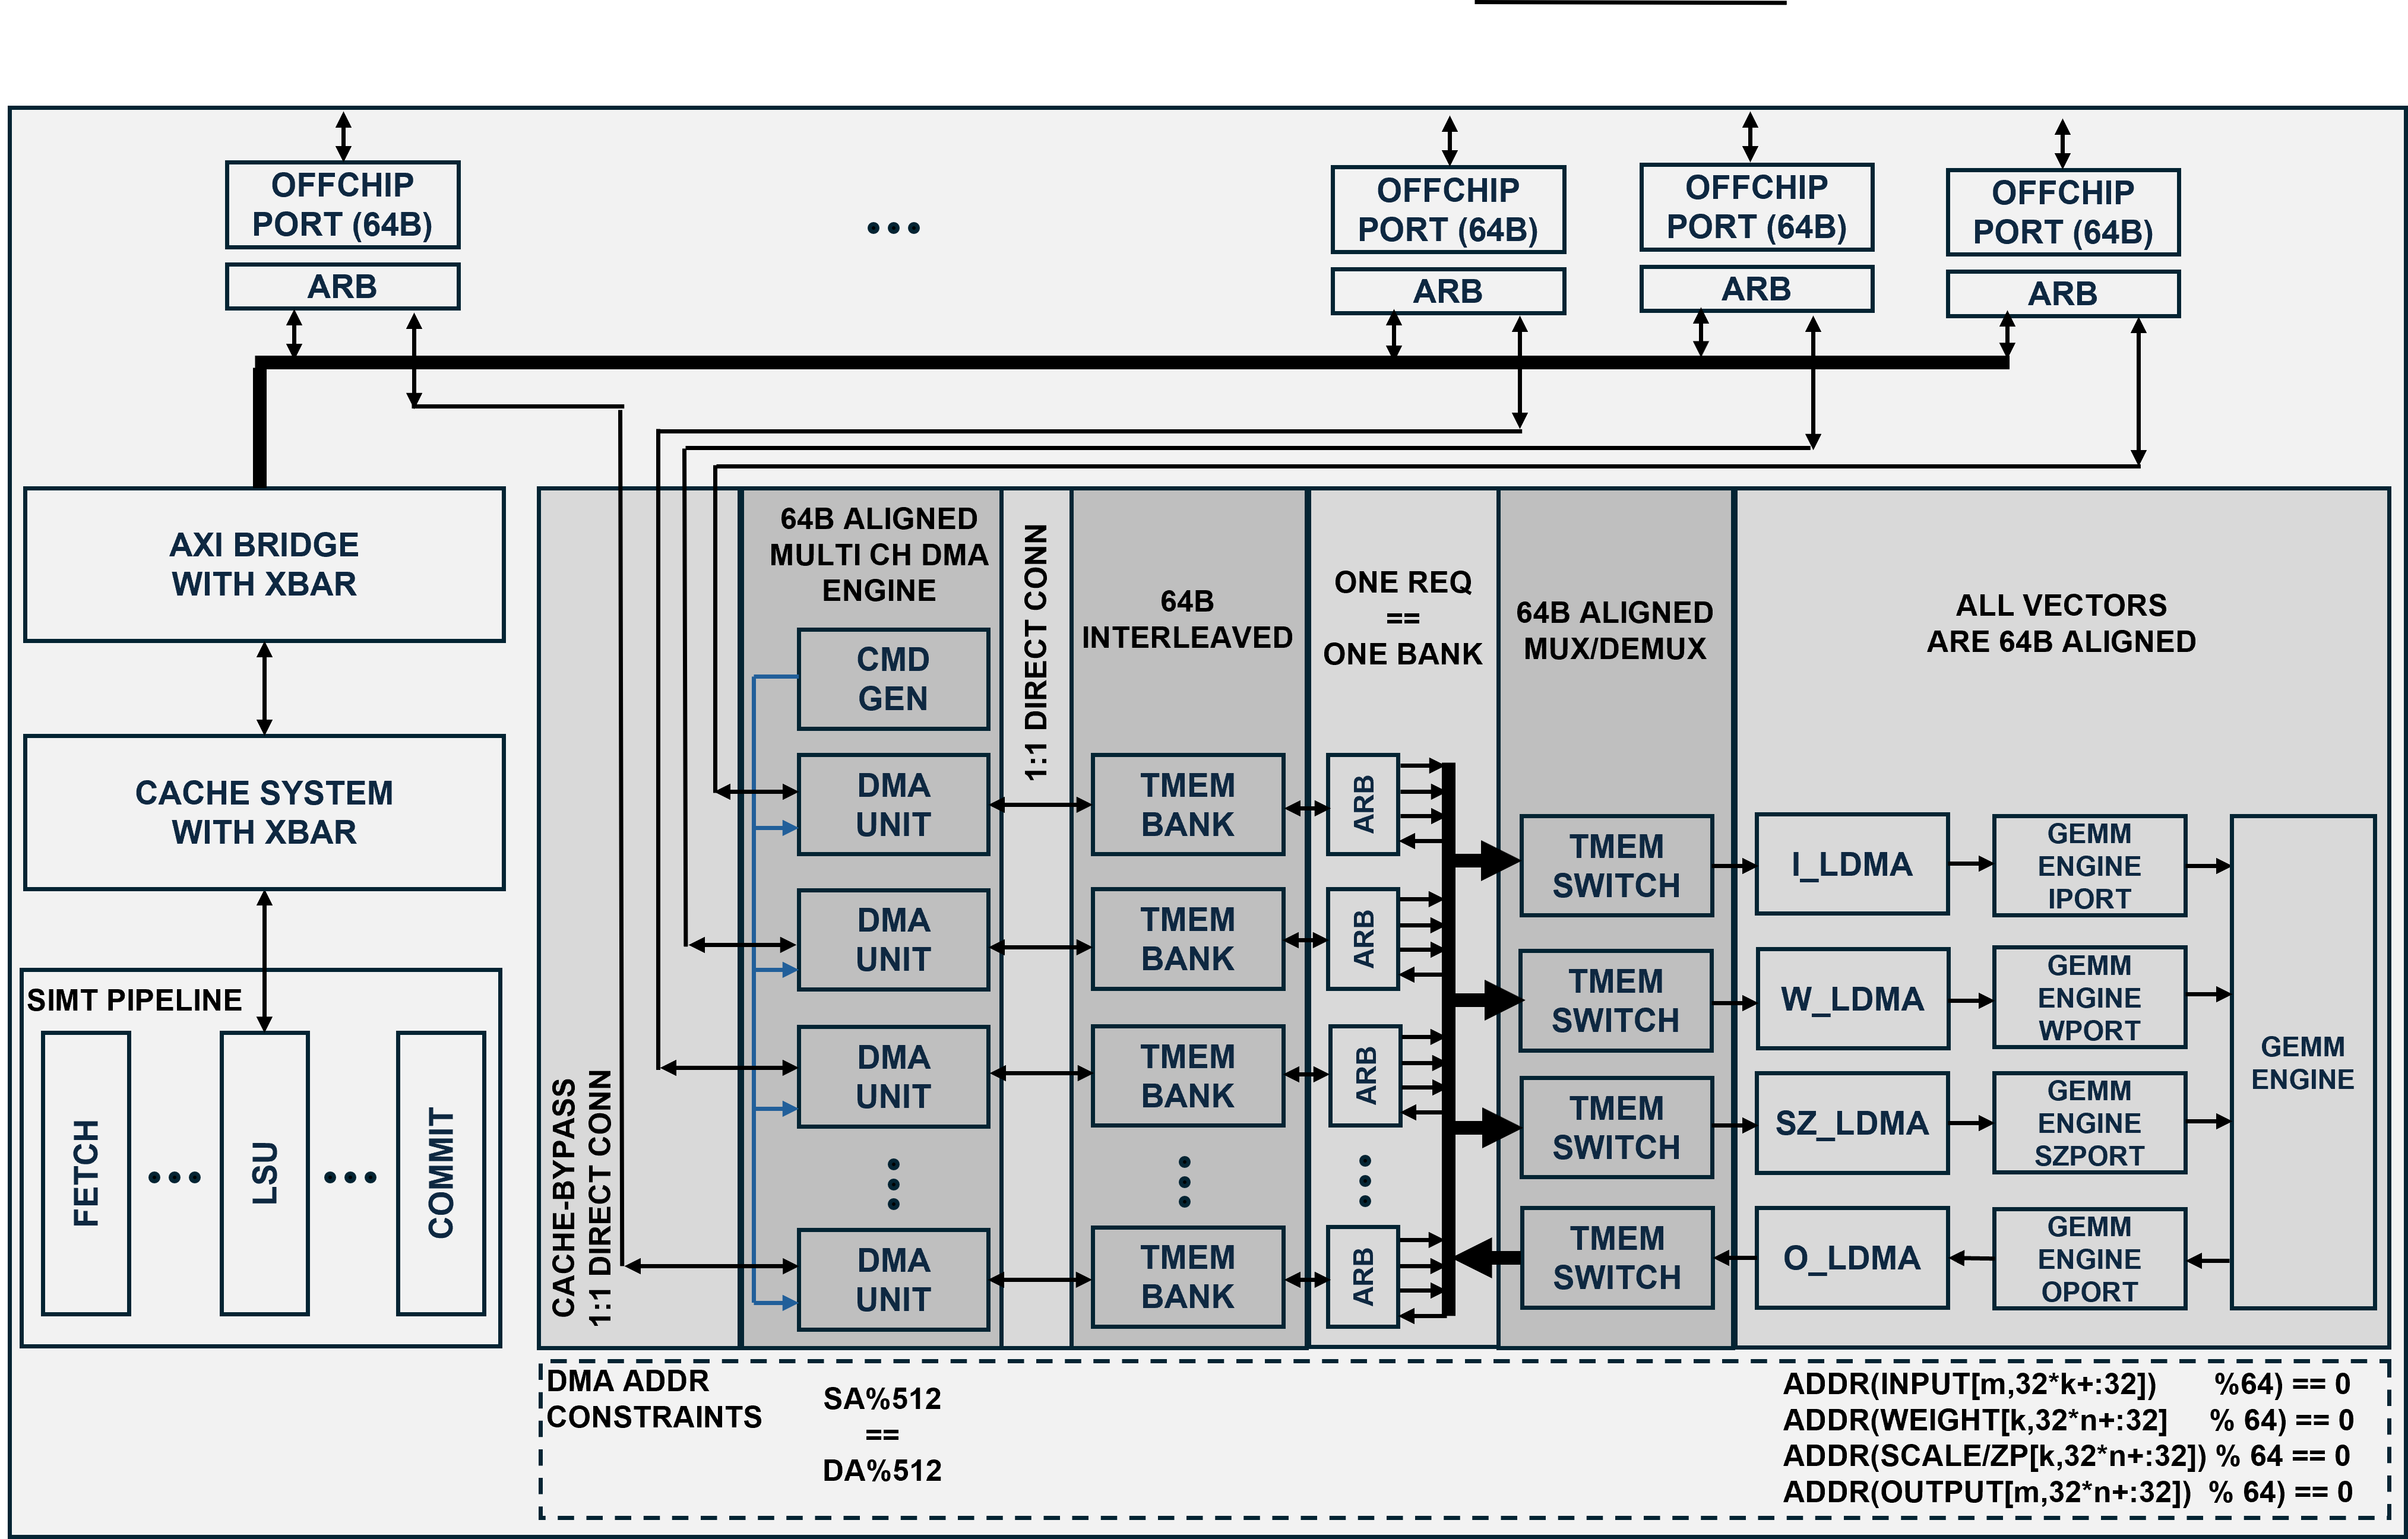
\includegraphics[width=0.92\linewidth]{figures/mem_sub_system.png}
%     \caption{Memory system for sustaining large \fpint{} arrays with direct tensor data movement.}
%     \label{fig:memory-system}
% \end{figure}
%\begin{figure*}[t]
%    \centering
%    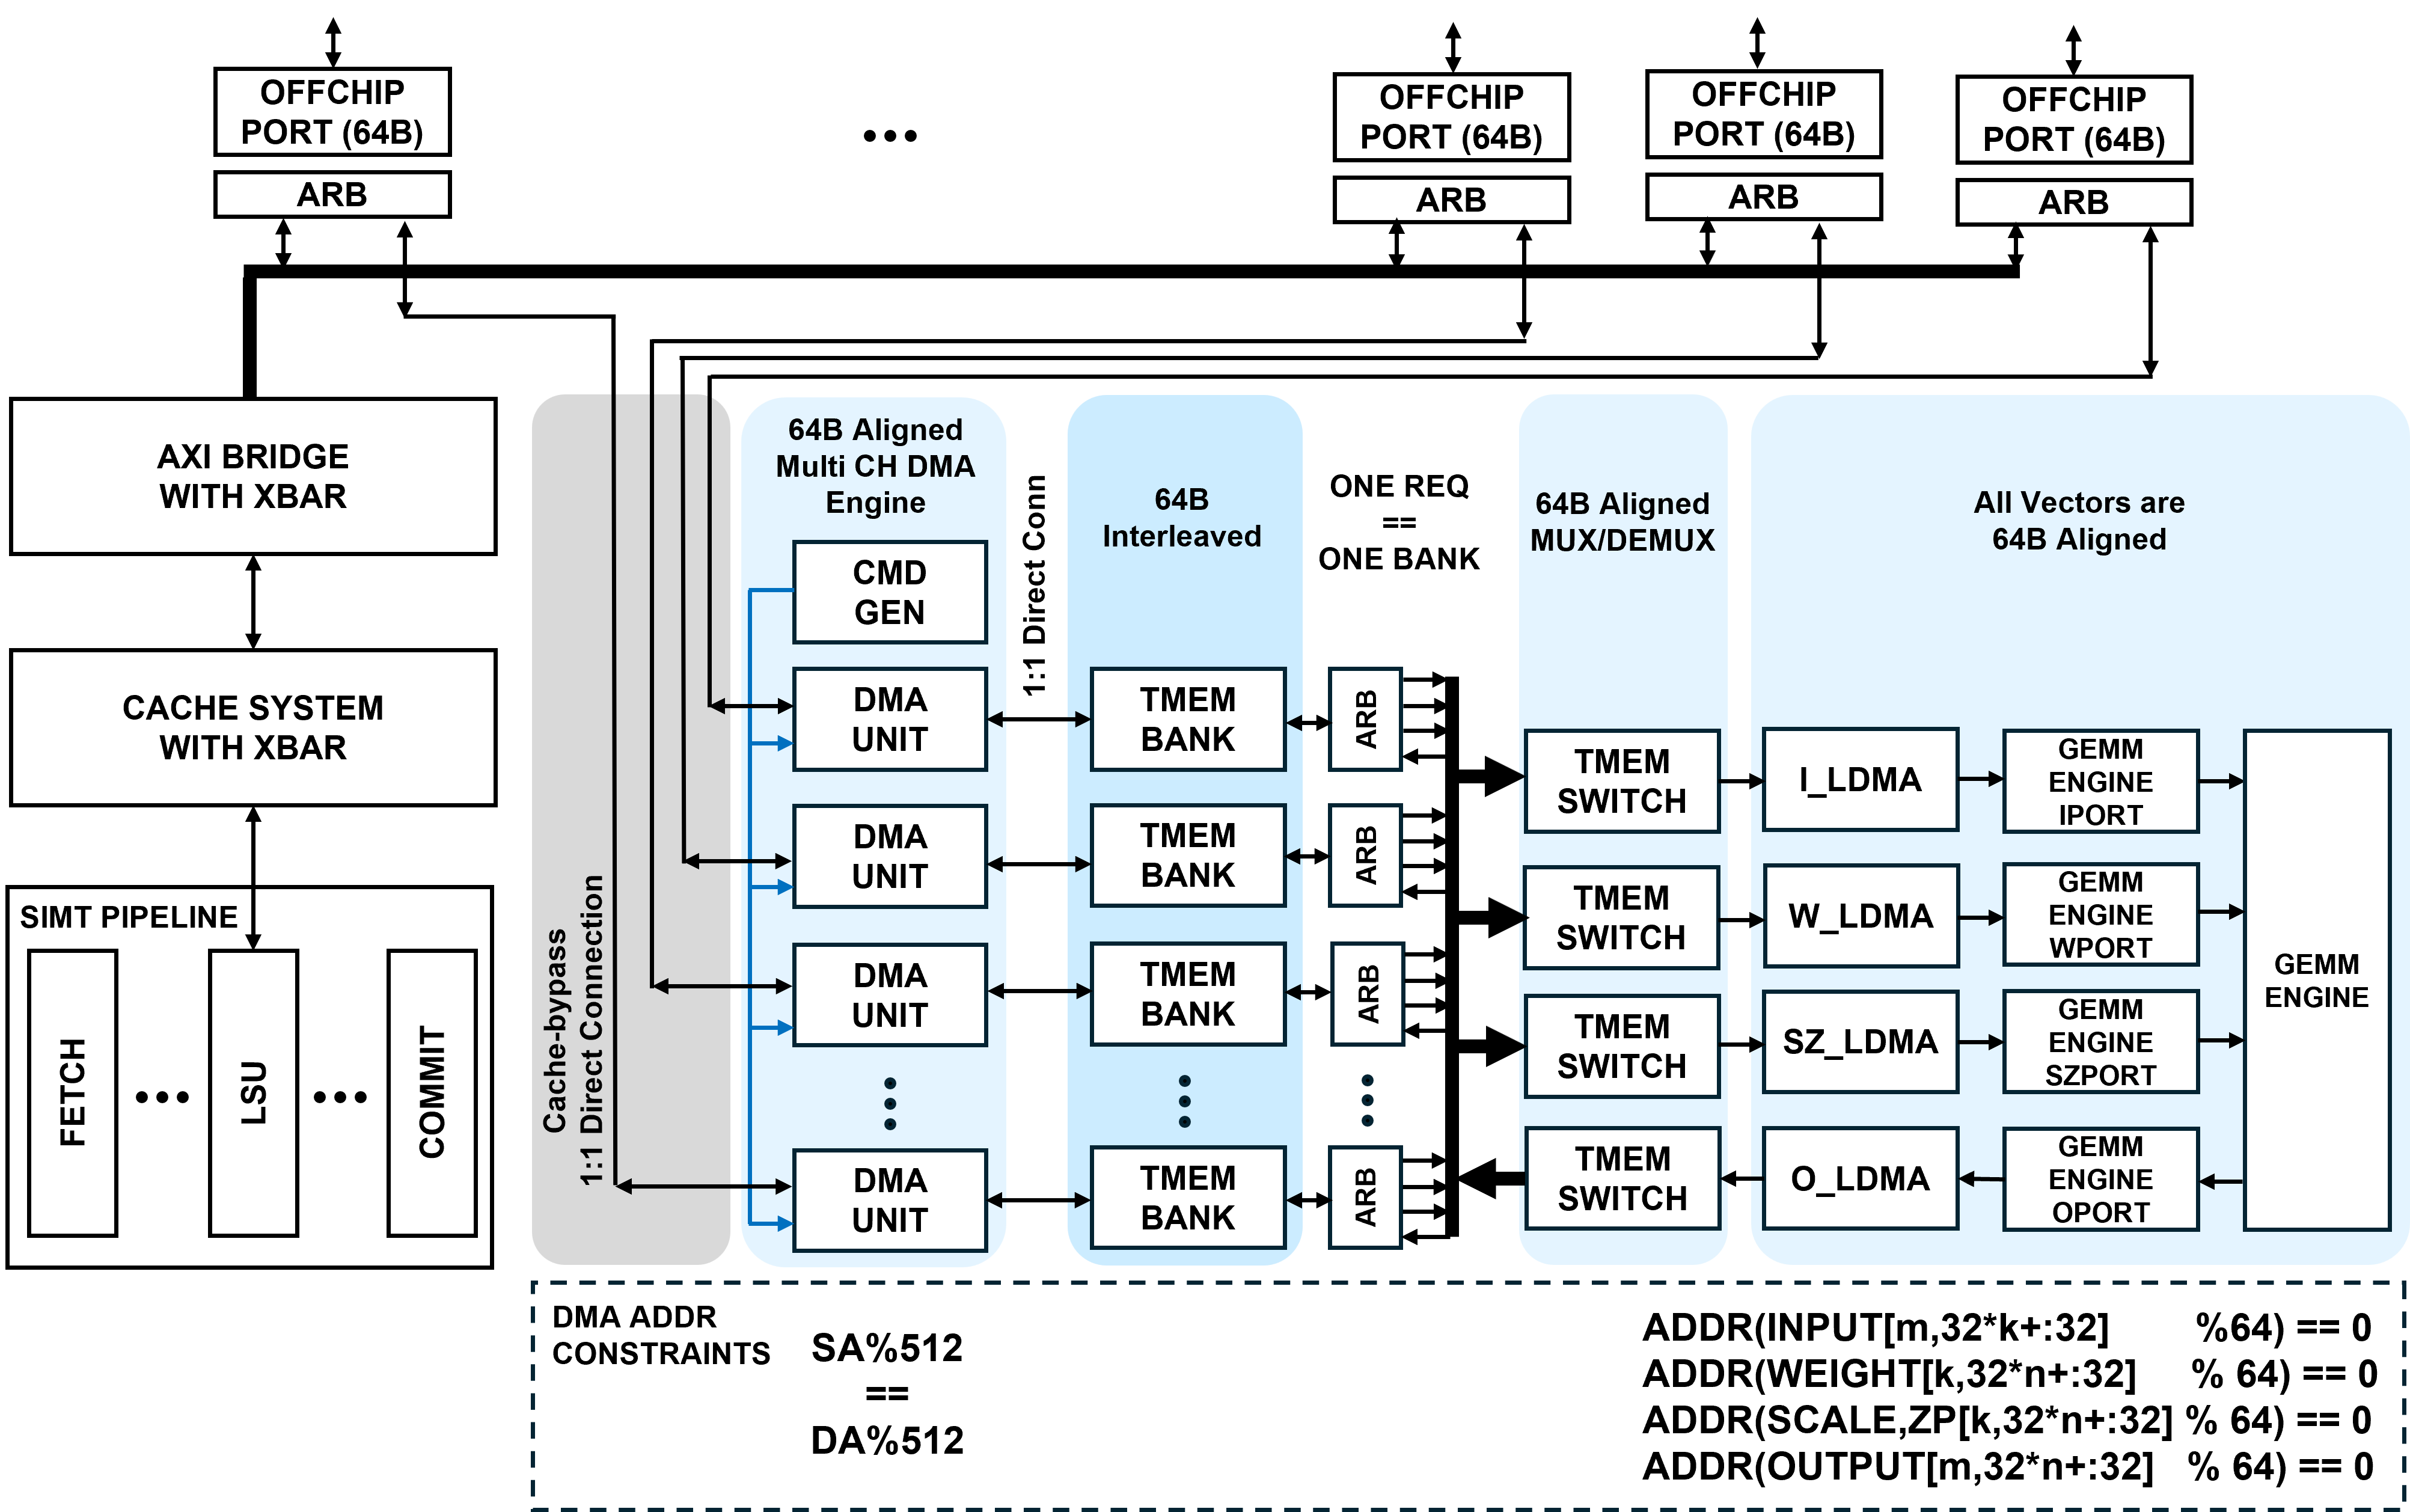
\includegraphics[width=0.96\textwidth]{figures/figs_fig9.png}
%    \caption{Memory system for sustaining large \fpint{} arrays with direct tensor data movement.}
%    \label{fig:memory-system}
%\end{figure*}

\begin{figure}[t]
    \centering
    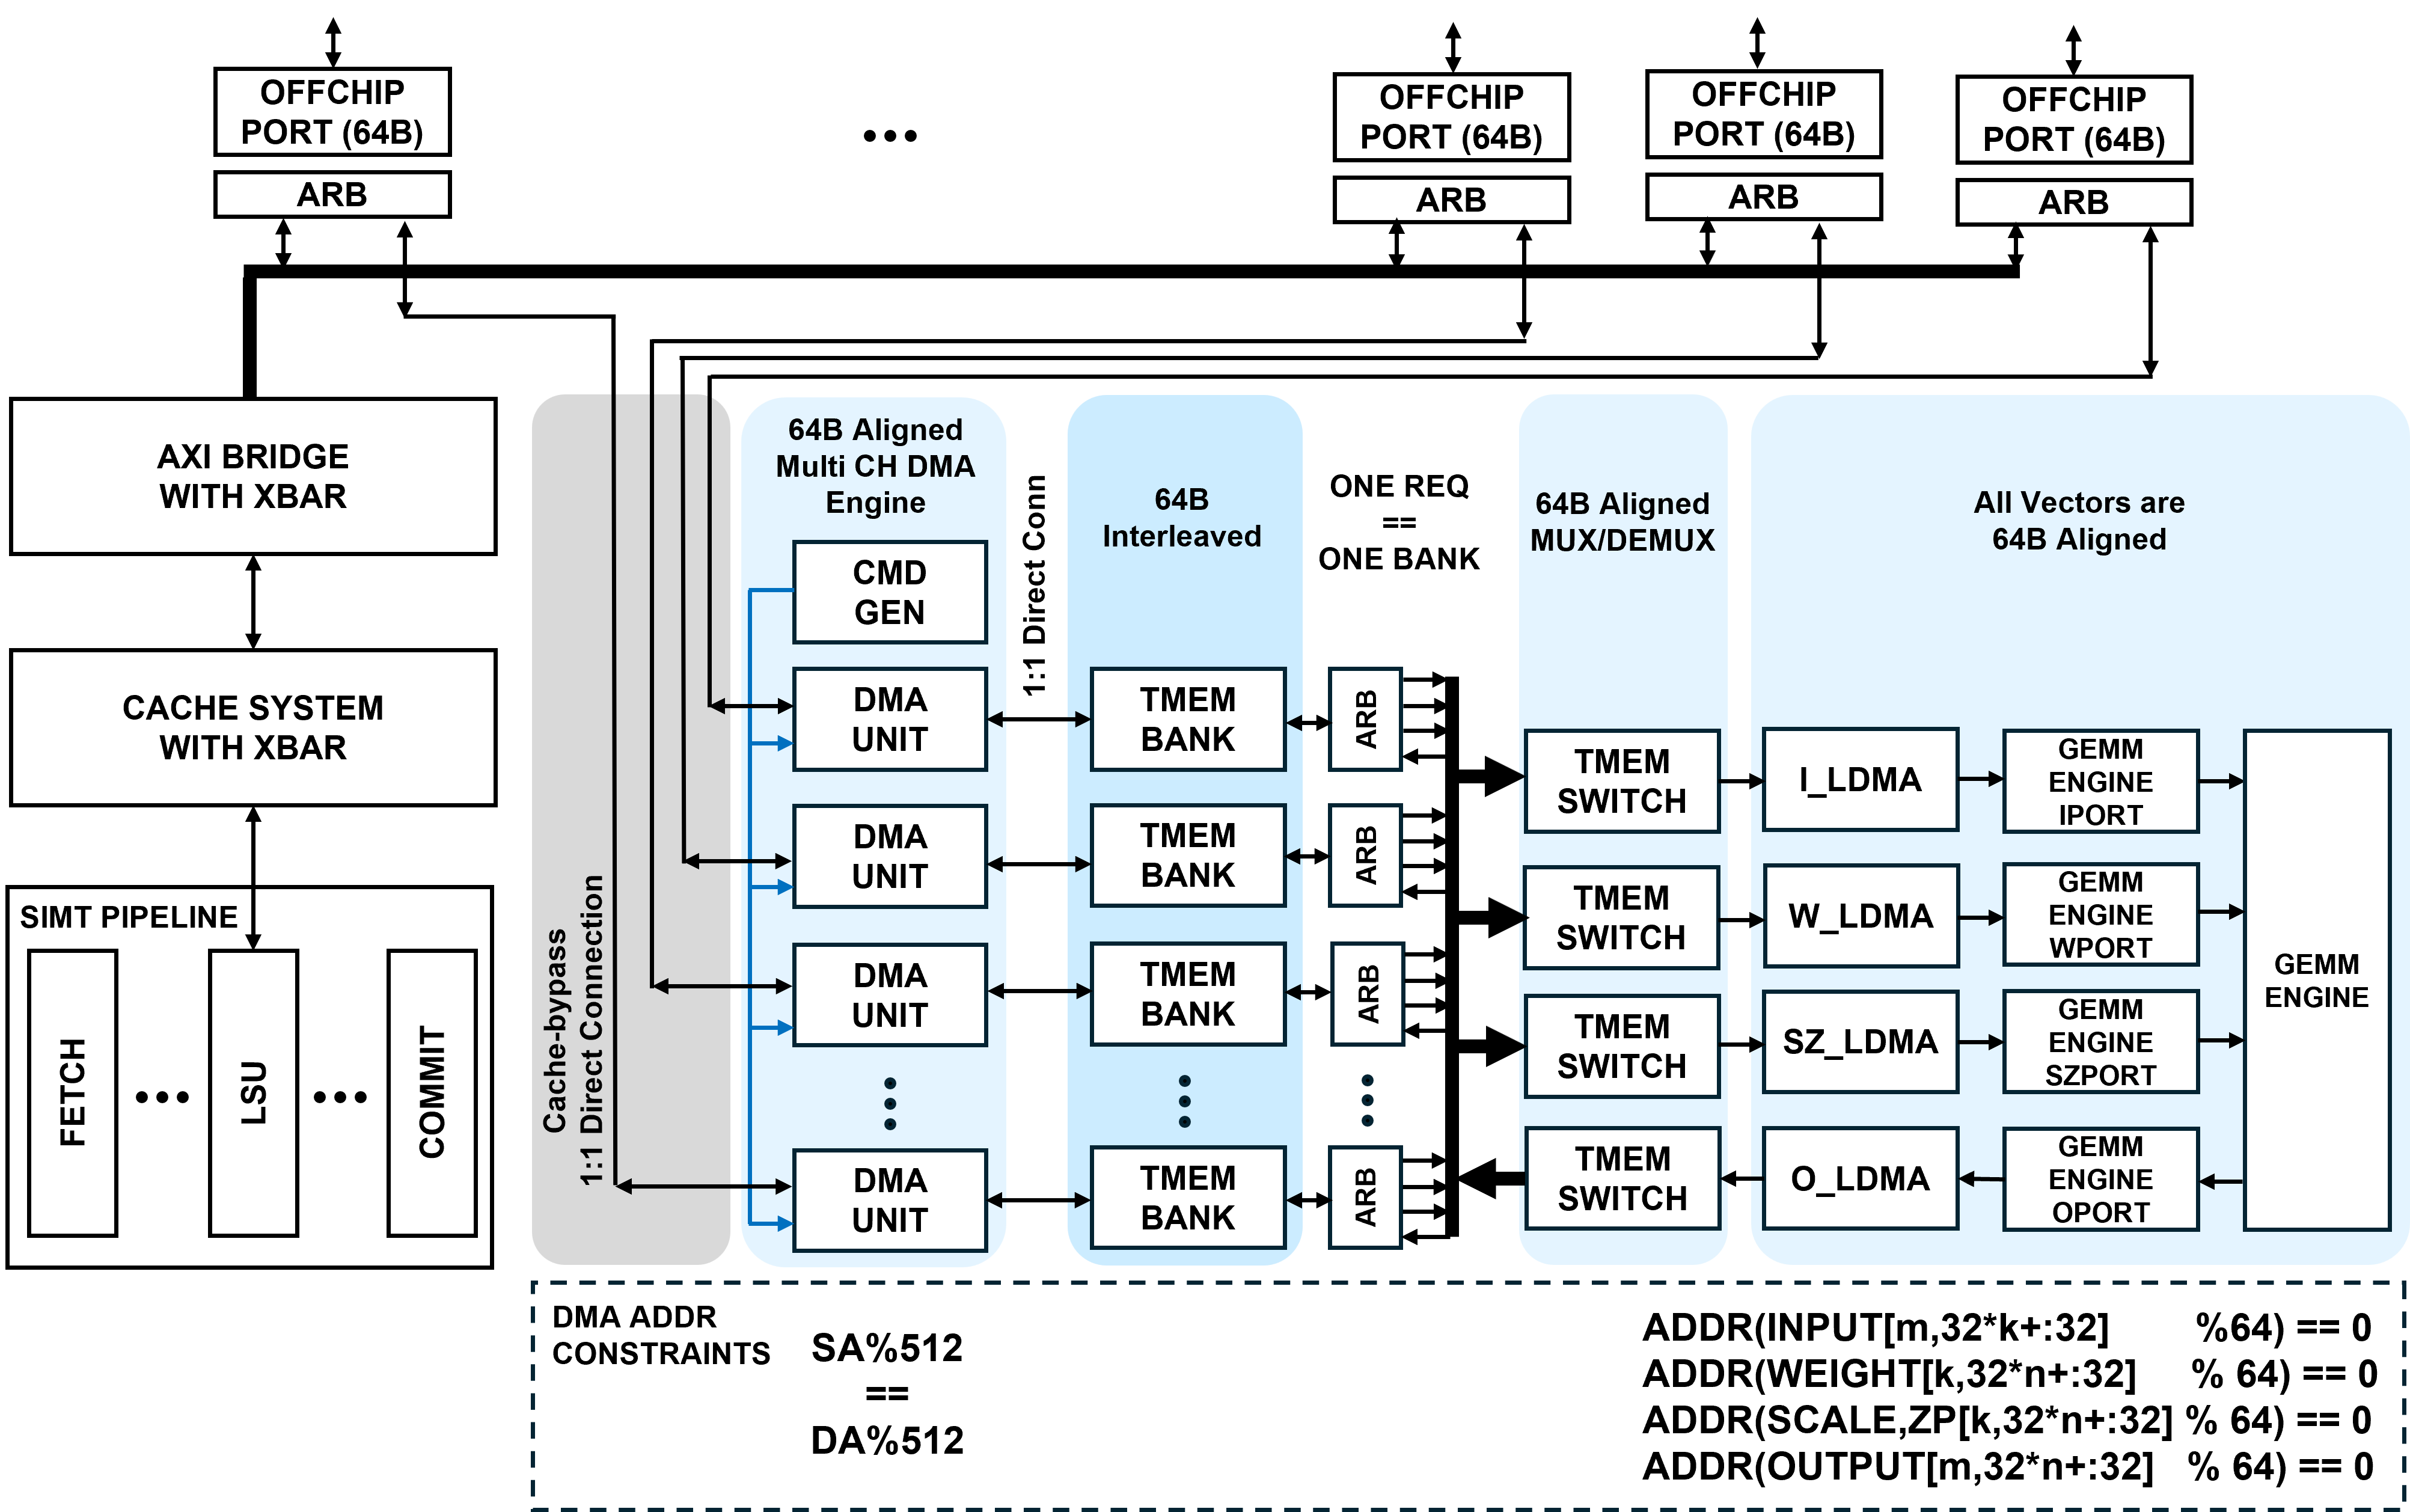
\includegraphics[width=0.92\linewidth]{figures/figs_fig9.png}
    \caption{Memory system for sustaining large \fpint{} arrays with direct tensor data movement.}
    \label{fig:memory-system}
\end{figure}

%\textbf{Cache-Bypassed Tensor DMA.}
\textbf{T-DMA and G-DMA.}
We refer to the DMA between HBM and TMEM as the Tile DMA (T-DMA), and to the DMA subsystem between TMEM and the GEMM engine as the GEMM Engine DMA (G-DMA).

The T-DMA moves tensor tiles directly between HBM pseudo-channels and TMEM banks through the fixed 1:1 or interleaved interconnect while bypassing the cache hierarchy. It intentionally supports only $DW$-byte-aligned requests. Supporting an arbitrary byte offset on this wide datapath would require either a $DW$-byte barrel shifter for single-cycle realignment or a multi-cycle realignment path with additional staging buffers. The latter would increase transfer latency and require more in-flight requests to sustain bandwidth. Restricting the interface to aligned requests avoids the datapath, buffering, and control needed solely for realignment; Section~\ref{sec:runtime-section} describes how tile-major layout satisfies this restriction. Cache bypass also prevents tensor traffic from contending with cache banks, local memory, and SIMT load/store traffic. Because the path is non-coherent with the cache hierarchy, the runtime ensures visibility using producer fences, result-tile completion polling, and cache management at kernel boundaries.

The G-DMA consists of four independent engines associated with the fixed 64\,B I, W, SZ, and O ports. The I, W, and SZ engines read input, weight, and scale/zero-point data from TMEM, whereas the O engine writes output data back to TMEM. Each engine can select any TMEM bank and transfers one aligned 64\,B port word at a time. With 4-bit weights and a 32$\times$32 MXU, each W-port transfer supplies four 32-element weight rows. Unlike the approximately ten-cycle local-memory path in the baseline GPU, TMEM is tightly coupled to the G-DMA and has a short, deterministic response latency. The G-DMA therefore needs fewer outstanding requests and shallower request queues to sustain its fixed port bandwidth. The four engines operate independently, allowing operand delivery and result writeback to proceed concurrently.

Overall, the aligned-only T-DMA removes wide realignment hardware on the HBM--TMEM path, while low-latency TMEM keeps the G-DMA request machinery shallow. Together with fixed interconnects and cache bypass, these specialized DMA engines prevent operand supply from limiting \fpint{} array utilization.

\begin{comment}
%We refer to the DMA between HBM and TMEM as the Tile DMA (T-DMA), and to the DMA subsystem between TMEM and the GEMM engine as the GEMM Engine DMA (G-DMA).
%The T-DMA moves aligned tensor tiles directly between HBM pseudo-channels and TMEM banks through the fixed 1:1 or interleaved interconnect, bypassing the cache hierarchy.
%Routing this traffic through the cache would force it to share paths with cache banks, local memory, and SIMT load/store traffic, turning crossbar and multi-bank arbitration into a bottleneck.
%The cache-bypassed path therefore reduces cache pollution and port conflicts.
%Because the T-DMA is non-coherent with the cache hierarchy, the runtime ensures visibility using producer fences, result-tile completion polling, and cache management at kernel boundaries.

%The G-DMA consists of four independent engines associated with the fixed 64\,B I, W, SZ, and O ports.
%The I, W, and SZ engines read input, weight, and scale/zero-point data from TMEM, whereas the O engine writes output data back to TMEM.
%Each engine can select any TMEM bank and transfers one aligned 64\,B port word at a time.
%With 4-bit weights and a 32$\times$32 MXU, each 64\,B W-port transfer supplies four 32-element weight rows.
%The four engines operate independently, allowing operand delivery and result writeback to proceed concurrently.

%Overall, descriptor-driven GEMM execution, partitioned tensor storage, fixed or interleaved HBM--TMEM connectivity, fixed-width G-DMA paths, and cache bypass prevent operand supply from limiting \fpint{} array utilization.


%Tensor traffic between HBM and TMEM banks also bypasses the cache hierarchy. Routing it through the cache would put it on paths shared with cache banks, local memory, and SIMT load/store, making crossbar and multi-bank arbitration costs the bottleneck again. \ours{} instead moves tensor data directly from HBM pseudo-channels to tensor memory banks, reducing cache pollution and port conflicts. Because this path is outside the coherent cache protocol, Section~\ref{sec:runtime-section} handles visibility through a producer fence, result tile completion polling, and mandatory cache management at kernel boundaries.
%Separately, between the TMEM banks and the GEMM engine, four independent I/W/SZ/O DMA engines transfer input, weight, scale/zero-point, and output tensors in parallel.
%Overall, descriptor-driven GEMM execution, partitioned tensor storage, interleaved-connected DMA, and cache bypass prevent \fpint{} array efficiency from being lost to operand supply.
\end{comment}

\section{Layout transformation and runtime optimization}
\label{sec:runtime-section}

The low-cost tensor path in Section~\ref{sec:memory-system} exposes two address constraints to software. A T-DMA transfer must satisfy both the HBM--TMEM endpoint-mapping constraint in Eq.~\ref{eq:general_interleaved_constraint} and the $DW$-byte alignment constraint in Eq.~\ref{eq:aligned_dma_constraint}. Independently, every G-DMA port word must satisfy the 64\,B TMEM alignment constraint in Eq.~\ref{eq:tmem_gemm_vector_constraint}. \ours{} regularizes these constraints through a power-of-two interconnect configuration, enforces them through alignment-aware allocation and tile-major layout, and removes most layout-conversion overhead through fusion.

\textbf{Power-of-Two Mapping and Aligned Allocation.}
\ours{} restricts the HBM pseudo-channel count $N_{\mathrm{pc}}$ and the TMEM bank count $N_{\mathrm{tmem}}$ to powers of two. The smaller count therefore divides the larger one. Define the HBM--TMEM mapping period as
\begin{equation}
    N_{\min}^{HT}
    =
    \min
    \left(
        N_{\mathrm{pc}},
        N_{\mathrm{tmem}}
    \right),
    \qquad
    P_{HT}
    =
    DW \cdot N_{\min}^{HT}.
    \label{eq:hbm_tmem_mapping_period}
\end{equation}
For the $DW$-aligned addresses required by Eq.~\ref{eq:aligned_dma_constraint}, the general endpoint-mapping constraint reduces to
\begin{equation}
    A_{\mathrm{HBM}}
    \equiv
    A_{\mathrm{TMEM}}
    \pmod{P_{HT}}.
    \label{eq:interleaved_address_constraint}
\end{equation}
\ours{} extends the Vortex runtime so an allocation can constrain both its size and base-address alignment. The runtime jointly selects the HBM and TMEM bases of each tile to satisfy Eq.~\ref{eq:interleaved_address_constraint}. Adding the same tile-local offset to both bases preserves the congruence, so all corresponding $DW$-byte words in a tile remain connected. Tile byte sizes are multiples of $P_{HT}$, and the tile layout places the base of every G-DMA port word at a multiple of 64\,B. Thus, successive T-DMA tiles preserve the HBM--TMEM mapping and every I/W/SZ/O port word begins at a legal TMEM address.

\textbf{Conflict-Free Tile-Major Layout.}
A padded row-major layout can satisfy both the address-congruence and alignment constraints above. Alignment alone therefore does not explain our choice of tile-major layout. The remaining problem is the bank-access sequence during a high-bandwidth tile transfer.

\begin{figure}[t]
   \centering

   \begin{subfigure}[t]{0.45\linewidth}
       \centering
       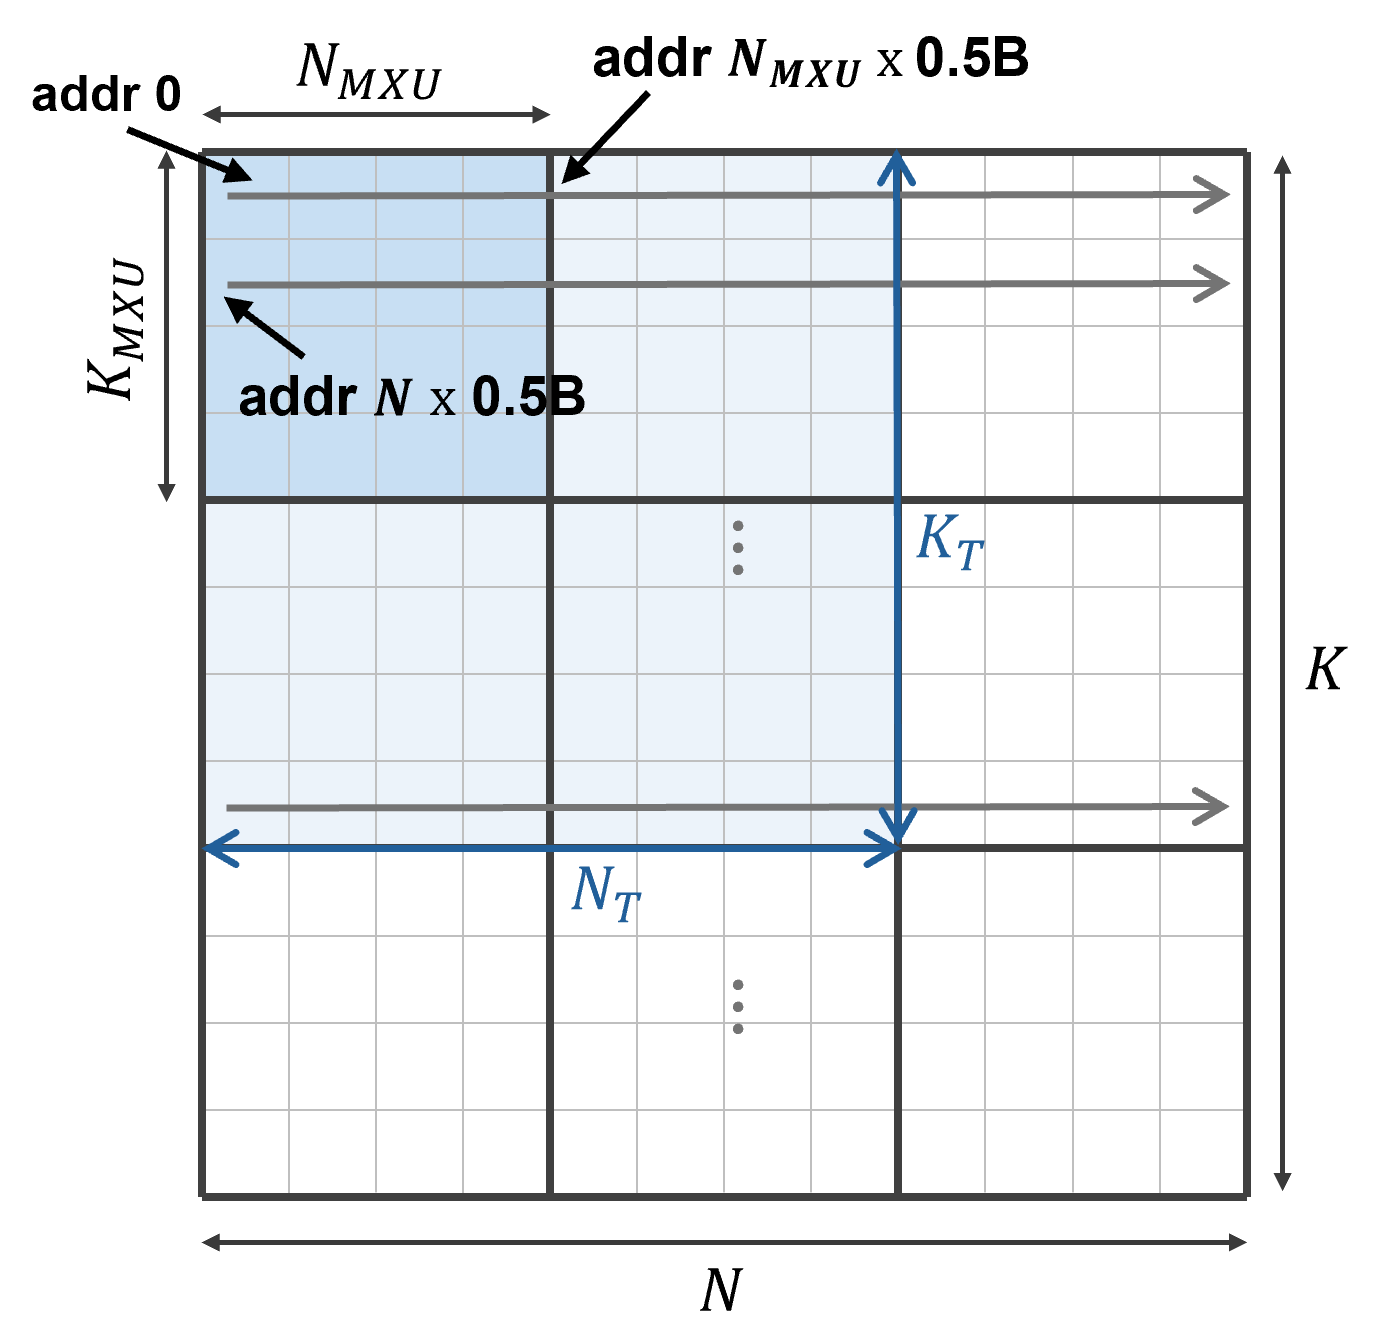
\includegraphics[width=\linewidth]{figures/tile-major-a.png}
       \caption{Row-major weight layout.}
       \label{fig:tile-major-a}
   \end{subfigure}
   \hfill
   \begin{subfigure}[t]{0.48\linewidth}
       \centering
       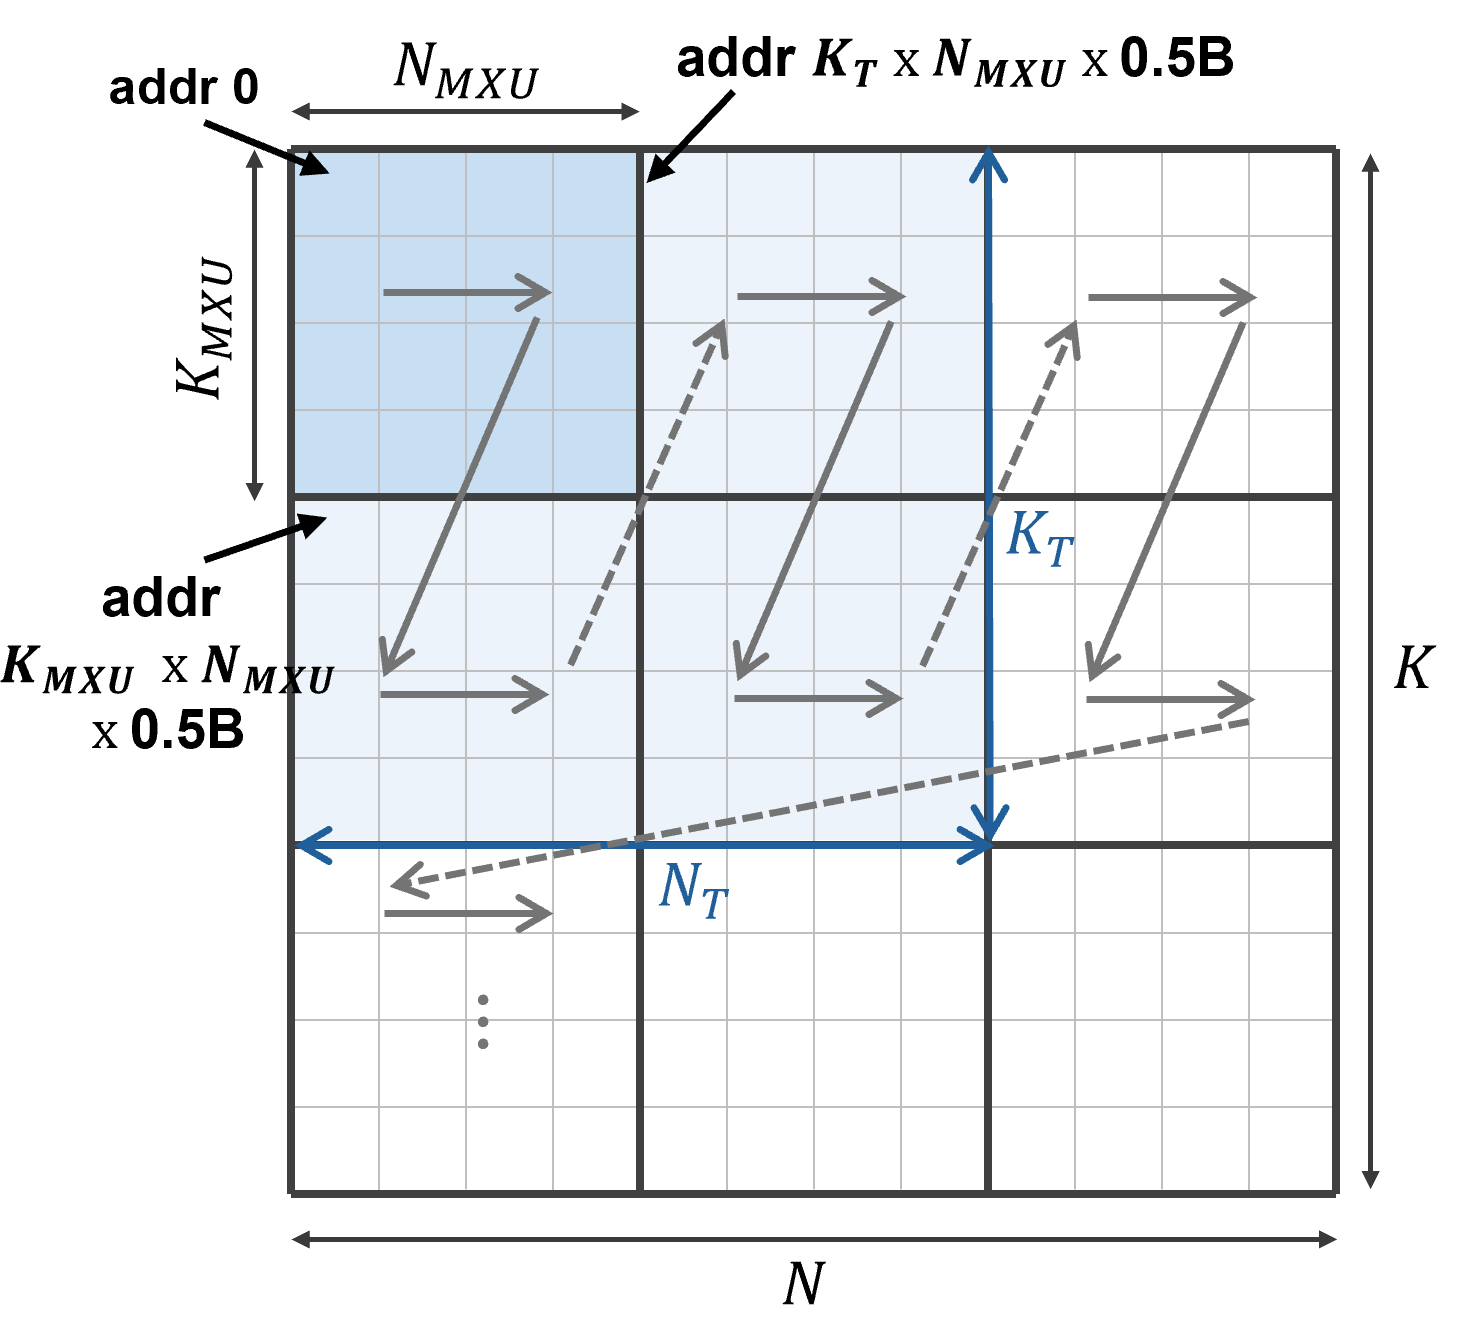
\includegraphics[width=\linewidth]{figures/tile-major-b.png}
       \caption{Tile-major weight layout.}
       \label{fig:tile-major-b}
   \end{subfigure}

   %\caption{In the row-major layout, a tile spans multiple noncontiguous row segments, whereas the tile-major input and weight layouts store each tile in a contiguous memory region.}
   \caption{Layout comparison for a representative weight tile. A row-major tile spans noncontiguous row segments, whereas tile-major storage makes the entire tile contiguous.}
   \label{fig:tile-major-layout}
\end{figure}

As shown in Fig.~\ref{fig:tile-major-a}, an $M_T \times K_T$ row-major tile consists of $M_T$ noncontiguous row segments. Within a segment, consecutive $DW$-byte words advance through consecutive banks. At a segment boundary, however, the address advances by the full padded row stride rather than by a tile-local contiguous offset. The next bank is therefore determined by the tensor shape and row stride, and multiple row segments issued in parallel may map to the same bank. Shape- and stride-dependent padding or bank-aware scheduling can avoid particular conflicts, but does not provide one general conflict-free mapping across supported tensor shapes.

In the tile-major layout of Fig.~\ref{fig:tile-major-b}, all words of a tile form one contiguous sequence. Under the low-order interleaving used by \ours{}, consecutive aligned words rotate across consecutive banks. A T-DMA tile transfer can therefore use one word from each bank per interleaving round without conflicts, up to the aggregate bank bandwidth. This predictable bank sequence, rather than alignment alone, is the primary reason that \ours{} uses tile-major storage.

\ours{} uses outer tile dimensions $M_T$, $K_T$, and $N_T$ for data transferred by the T-DMA and inner tile dimensions $M_{\mathrm{MXU}}$, $K_{\mathrm{MXU}}$, and $N_{\mathrm{MXU}}$ for data consumed through the G-DMA. Besides guaranteeing the address properties above, contiguous storage lets the runtime describe a tile as one aligned transfer rather than as separate requests for its row segments.
It directly satisfies the aligned-only T-DMA interface.
%The T-DMA therefore requires neither per-row gather support nor a misalignment-realignment datapath.

\ours{} uses outer tile dimensions $M_T$, $K_T$, and $N_T$ for data transferred by the T-DMA and inner tile dimensions $M_{\mathrm{MXU}}$, $K_{\mathrm{MXU}}$, and $N_{\mathrm{MXU}}$ for data consumed through the G-DMA. Besides guaranteeing the address properties above, contiguous storage lets the runtime describe a tile with one aligned descriptor rather than separate requests for its row segments, directly satisfying the aligned-only T-DMA interface.

\textbf{Fused Layout Transformation.}
Converting every tensor with a separate layout-transformation kernel would add an extra memory pass and could offset the benefit of the tensor path. Static weights are remapped to tile-major form offline. For dynamically produced activations and outputs, \ours{} fuses layout transformation into vector kernels that are adjacent to a GEMM in the computation graph. Examples include RMSNorm, RoPE, softmax, and residual addition when they directly precede or follow a GEMM, as illustrated in Fig.~\ref{fig:fuse_layout_transform}. A preceding vector kernel writes its output directly in aligned tile-major form, whereas a following vector kernel consumes the tile-major GEMM output as part of its normal computation. The resulting tensor objects and descriptors can therefore be passed through the T-DMA and G-DMA without a standalone layout-conversion pass at the GEMM boundary.

\begin{figure}[t]
    \centering
    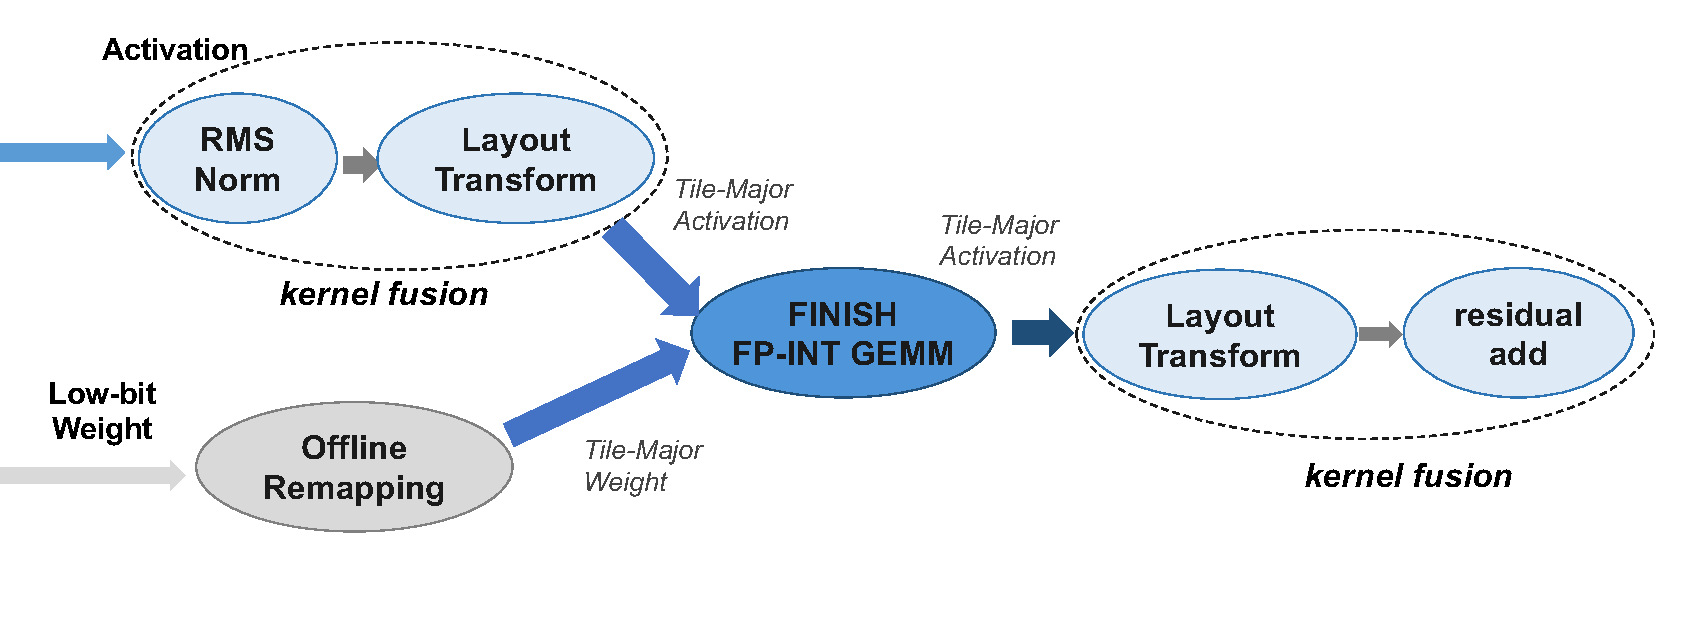
\includegraphics[width=0.92\linewidth]{figures/fig9_layout_fusion.pdf}
    \caption{Fused layout transformation for producing T-DMA-compatible tile-major tensors. The figure shows representative offline and fused transformation sites.}
    \label{fig:fuse_layout_transform}
\end{figure}

\begin{comment}
%The memory system of Section~\ref{sec:memory-system} simplifies hardware at the cost of three software-visible constraints: address alignment, bank mapping, and non-coherent DMA. \ours{} satisfies them by exploiting GEMM's regular tile-access pattern with tile-major layout, fused layout transformation, and alignment-aware allocation. Instead of relying on a complex interconnect, the software keeps both tensor layout and placement in a hardware-friendly form.
 
%\textbf{Tile-major Layout and Aligned Allocation.}
%\ours{} meets the constraints of Section~\ref{sec:memory-system} by changing the tensor layout to a tile-major form, choosing tile sizes appropriately, and jointly controlling the base address at which the tile is allocated in memory.

% \begin{figure}[t]
%    \centering
%    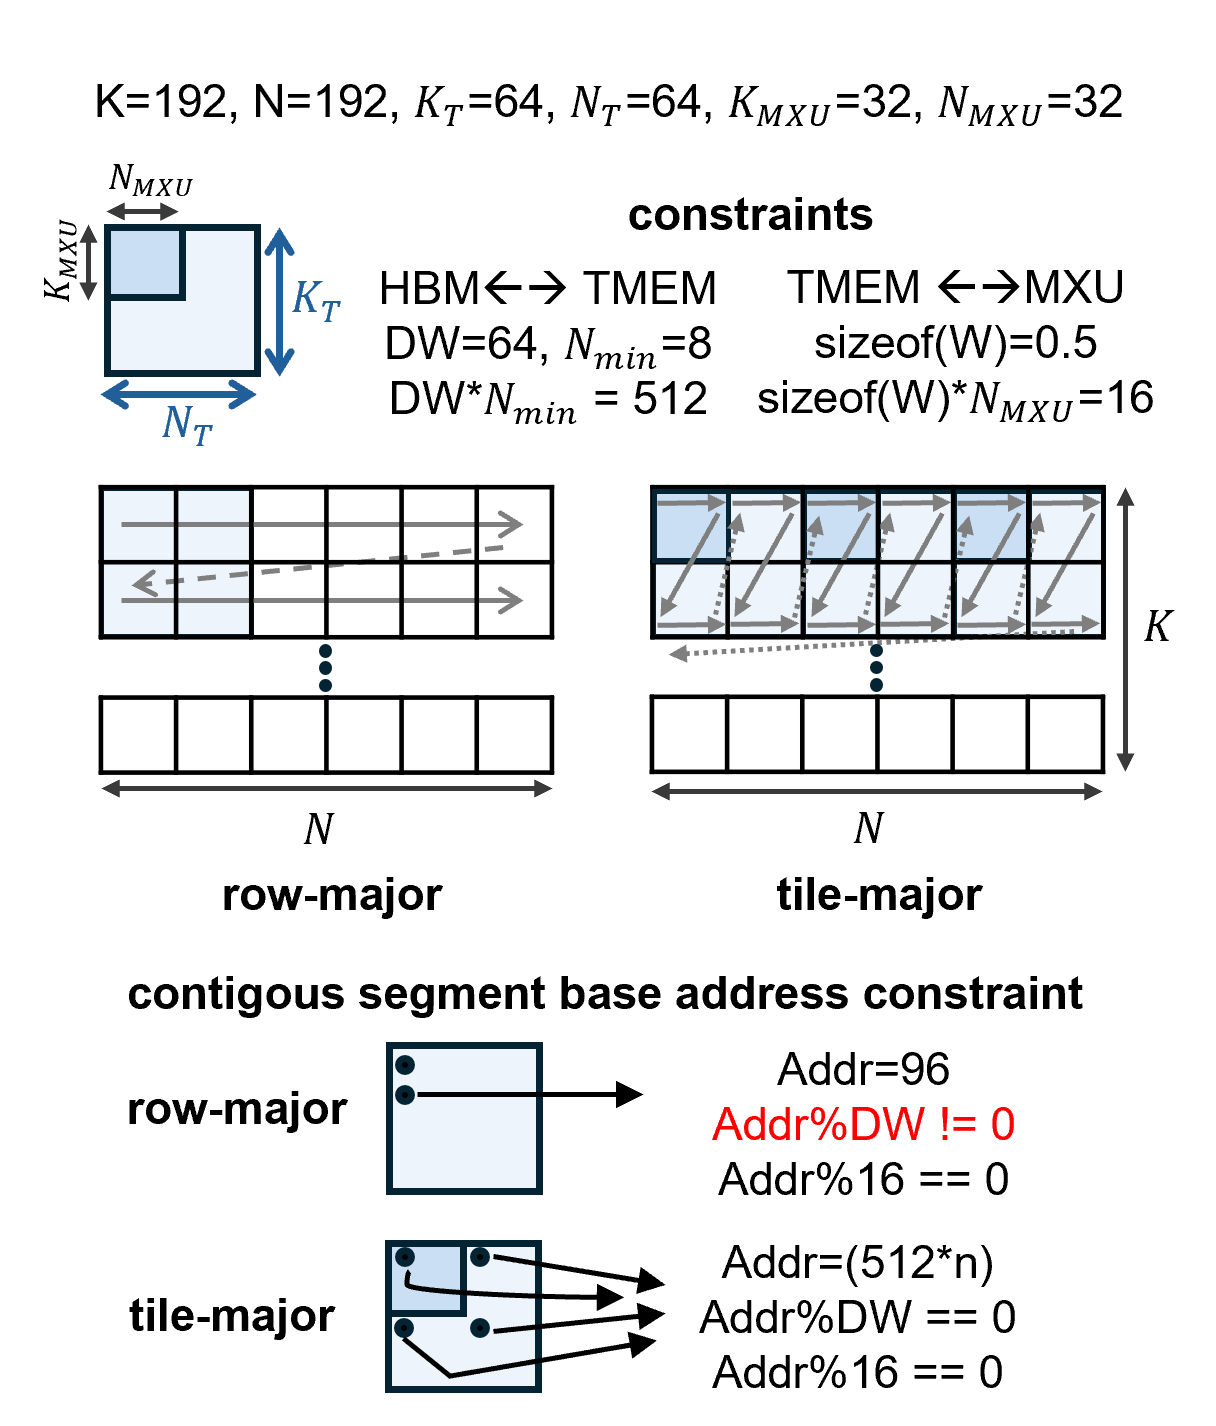
\includegraphics[width=0.9\linewidth]{figures/layout.png}
%    \caption{In the row-major layout, a tile spans multiple noncontiguous row segments, whereas the tile-major input and weight layouts store each tile in a contiguous memory region.}
%    \label{fig:tile-major-layout}
% \end{figure}

%\ours{} launches a SIMT kernel that transforms GEMM input and output tensors into a format organized by tiles. The layout uses tile dimensions $M_T$, $K_T$, and $N_T$ for data transferred from HBM to tensor memory. It uses a second tile shape, defined by $M_{\mathrm{MXU}}$, $K_{\mathrm{MXU}}$ and $N_{\mathrm{MXU}}$, for operand tiles consumed by the GEMM engine from tensor memory. 
%Each tile size is a multiple of the relevant mapping and vector-alignment moduli above, and elements within a tile are contiguous, so the address constraints are met by construction.
%Each tile size is a multiple of the alignment granularity moduli specified in Section~\ref{sec:memory-system}, and elements within a tile are contiguous, so the address constraints are met by construction.

%Figure~\ref{fig:tile-major-layout} illustrates how the tile-major layout enables an efficient high-bandwidth DMA implementation. In the row-major layout shown in Fig.~\ref{fig:tile-major-a}, an $M_T \times K_T$ tile is distributed across $M_T$ noncontiguous row segments. Because the base address of each segment is determined by the full row stride, these segments are not necessarily aligned to the wide DMA datapath. The DMA must therefore support misaligned accesses. Although realignment is relatively inexpensive for a narrow datapath, its hardware cost grows substantially as the DMA width increases: a single-cycle implementation requires a wide barrel shifter, whereas a multi-cycle implementation increases transfer latency. Hiding this additional latency requires more outstanding-request buffer entries, further increasing the area and complexity of the DMA engine.
%Moreover, because the row segments are noncontiguous in a row-major layout, an interleaved memory address mapping may map multiple segments to the same bank, increasing the likelihood of bank conflicts.
%In contrast, the tile-major layout in Fig.~\ref{fig:tile-major-b} stores all $M_T \times K_T$ elements of a tile contiguously and aligns each tile to the DMA transfer width. The tile can therefore be transferred using an aligned-only DMA without a wide realignment datapath or additional buffering for multi-cycle misaligned accesses.
%In contrast, the tile-major layout stores addresses within each tile contiguously, guaranteeing conflict-free bank accesses unless the requested bandwidth exceeds the aggregate bank bandwidth.
%As shown in Fig.~\ref{fig:tile-major-c}, FINISH applies the same organization to the weight tensor. Moreover, because TMEM is a tightly coupled memory with a short request-to-response latency, unlike GPU local memory whose access latency is approximately ten cycles, the TMEM--MXU DMA requires fewer outstanding requests to sustain bandwidth. Together, aligned tile-major accesses and low-latency TMEM enable a simpler and more efficient high-bandwidth DMA implementation.

%Figure~\ref{fig:tile-major-layout} illustrates how this organization reduces DMA command overhead. In the row-major layout shown in Fig.~\ref{fig:tile-major-a}, an $M_T \times K_T$ tile is divided across $M_T$ noncontiguous row segments. For illustration, assume that the tile begins at address 0, each element occupies 2 bytes, and each row contains $K$ elements. The DMA transfers the first $K_T$ elements by issuing a $K_T \times 2$ bytes request at address 0. It then transfers the second row segment by issuing another $K_T \times 2$-byte request at address $K \times 2$. Repeating this process for all rows requires a total of $M_T$ DMA commands. In contrast, the tile-major layout in Fig.~\ref{fig:tile-major-b} stores all $M_T \times K_T$ elements of the tile contiguously. The DMA can therefore fetch the entire tile from address 0 using a single command that transfers $M_T \times K_T \times 2$ bytes. As shown in Fig.~\ref{fig:tile-major-c}, \ours{} applies the same organization to the weight tensor.

%\ours{} extends the Vortex runtime so memory allocation can constrain both requested size and base-address alignment. The runtime applies this constraint jointly to HBM and tensor-memory allocations so Eq.~\ref{eq:interleaved_address_constraint} holds. Kernels pass aligned tensor objects and tile descriptors to the DMA rather than arbitrary pointers, allowing the DMA to issue aligned bursts without a wide barrel shifter or general crossbar.

%Tile-major layout and alignment also improve DMA efficiency. A DMA request is most efficient when it moves a large contiguous segment; repeated small row-major or column-major requests create bubbles on long-latency paths. With tile-major layout, the requested tile is contiguous and can be described by a single command. Multiple DMA units then auto-generate addresses from stride and bound information and fetch the tensor region in parallel, while the simple channel-to-bank mapping keeps controller logic small.

%\textbf{Cache Visibility in Fused Kernels.}
%We describe cache visibility for kernels that fuse vector stages with GEMM. When a vector stage precedes GEMM, it finishes producing the GEMM inputs and then issues a Vortex fence. This fence drains pending stores and flushes cached data to HBM before GEMM begins reading its inputs. When a vector stage follows GEMM, it does not need another fence. The GEMM node uses its result writeback DMA to move each completed accumulator tile directly to HBM through the cache bypass path. The node updates a read only MMIO completion register only after the corresponding HBM write completes. Downstream SIMT code polls this register for its target tile and starts computation after observing completion. Because the result writeback DMA does not allocate cache lines, the following SIMT load obtains the completed tile from HBM. Vortex also invalidates the cache at the beginning of every kernel launch and forces a fence at the end of every kernel. The final fence flushes cached writes before control returns to the runtime. These mechanisms allow GEMM to overlap with fused vector stages without requiring a hardware coherence protocol.
 
%\textbf{Fused Layout Transformation.}
%Running layout transformation as a separate kernel would add a memory pass that can offset the gains of the tensor path. As shown in Figure~\ref{fig:fuse_layout_transform}, \ours{} fuses the transform into surrounding kernels such as Q/K/V projection, quantization, GEMM preparation, and output movement. Tensors are written to HBM in a layout suited to DMA, and the requirements of the interleaved tensor path are satisfied.
\end{comment}

\section{Evaluation}

\subsection{Methodology}
\textbf{Hardware Evaluation Setup.}
We compare four hardware candidates.

\begin{itemize}
    \item \textit{C1: \Cone{}.}
    Implemented by enabling an FP$\times$FP TCU on Vortex.
    C1 executes all GEMM operations on the FP TCU after
    dequantizing the INT-quantized operands on the SIMT core.

    \item \textit{C2: \Ctwo{}.}
    We add a decoupled \fpint{} MXU on top of C1.
    The QKV generation and the FFN linear projections are
    executed on the \fpint{} MXU, while the $QK^T$ and PV
    operations of attention are executed on the FP TCU.
    C2 represents prior work such as FIGNA/FIGLUT/LUT-TC
    that accelerates only linear operations with \fpint{}.

    \item \textit{C3: \Cthr{}.}
    Both linear layers and the $QK^T$ and PV attention operations execute
    on the \fpint{} MXU, but the memory subsystem, runtime, and tensor
    layout remain unoptimized. C3 minimizes changes to the Vortex memory
    system by allowing the GEMM engine to share the existing local-memory
    and cache paths. It uses a conventional row-major layout without
    padding and relies on DMA support for misaligned accesses to move data
    between HBM and local memory and between local memory and the GEMM
    engine.

    \item \textit{C4: \ours{}.}
    Final design with \fpint{} execution for both linear and
    attention kernels, together with the memory subsystem,
    runtime, and layout optimizations.
\end{itemize}

\begin{figure}[t]
    \centering
    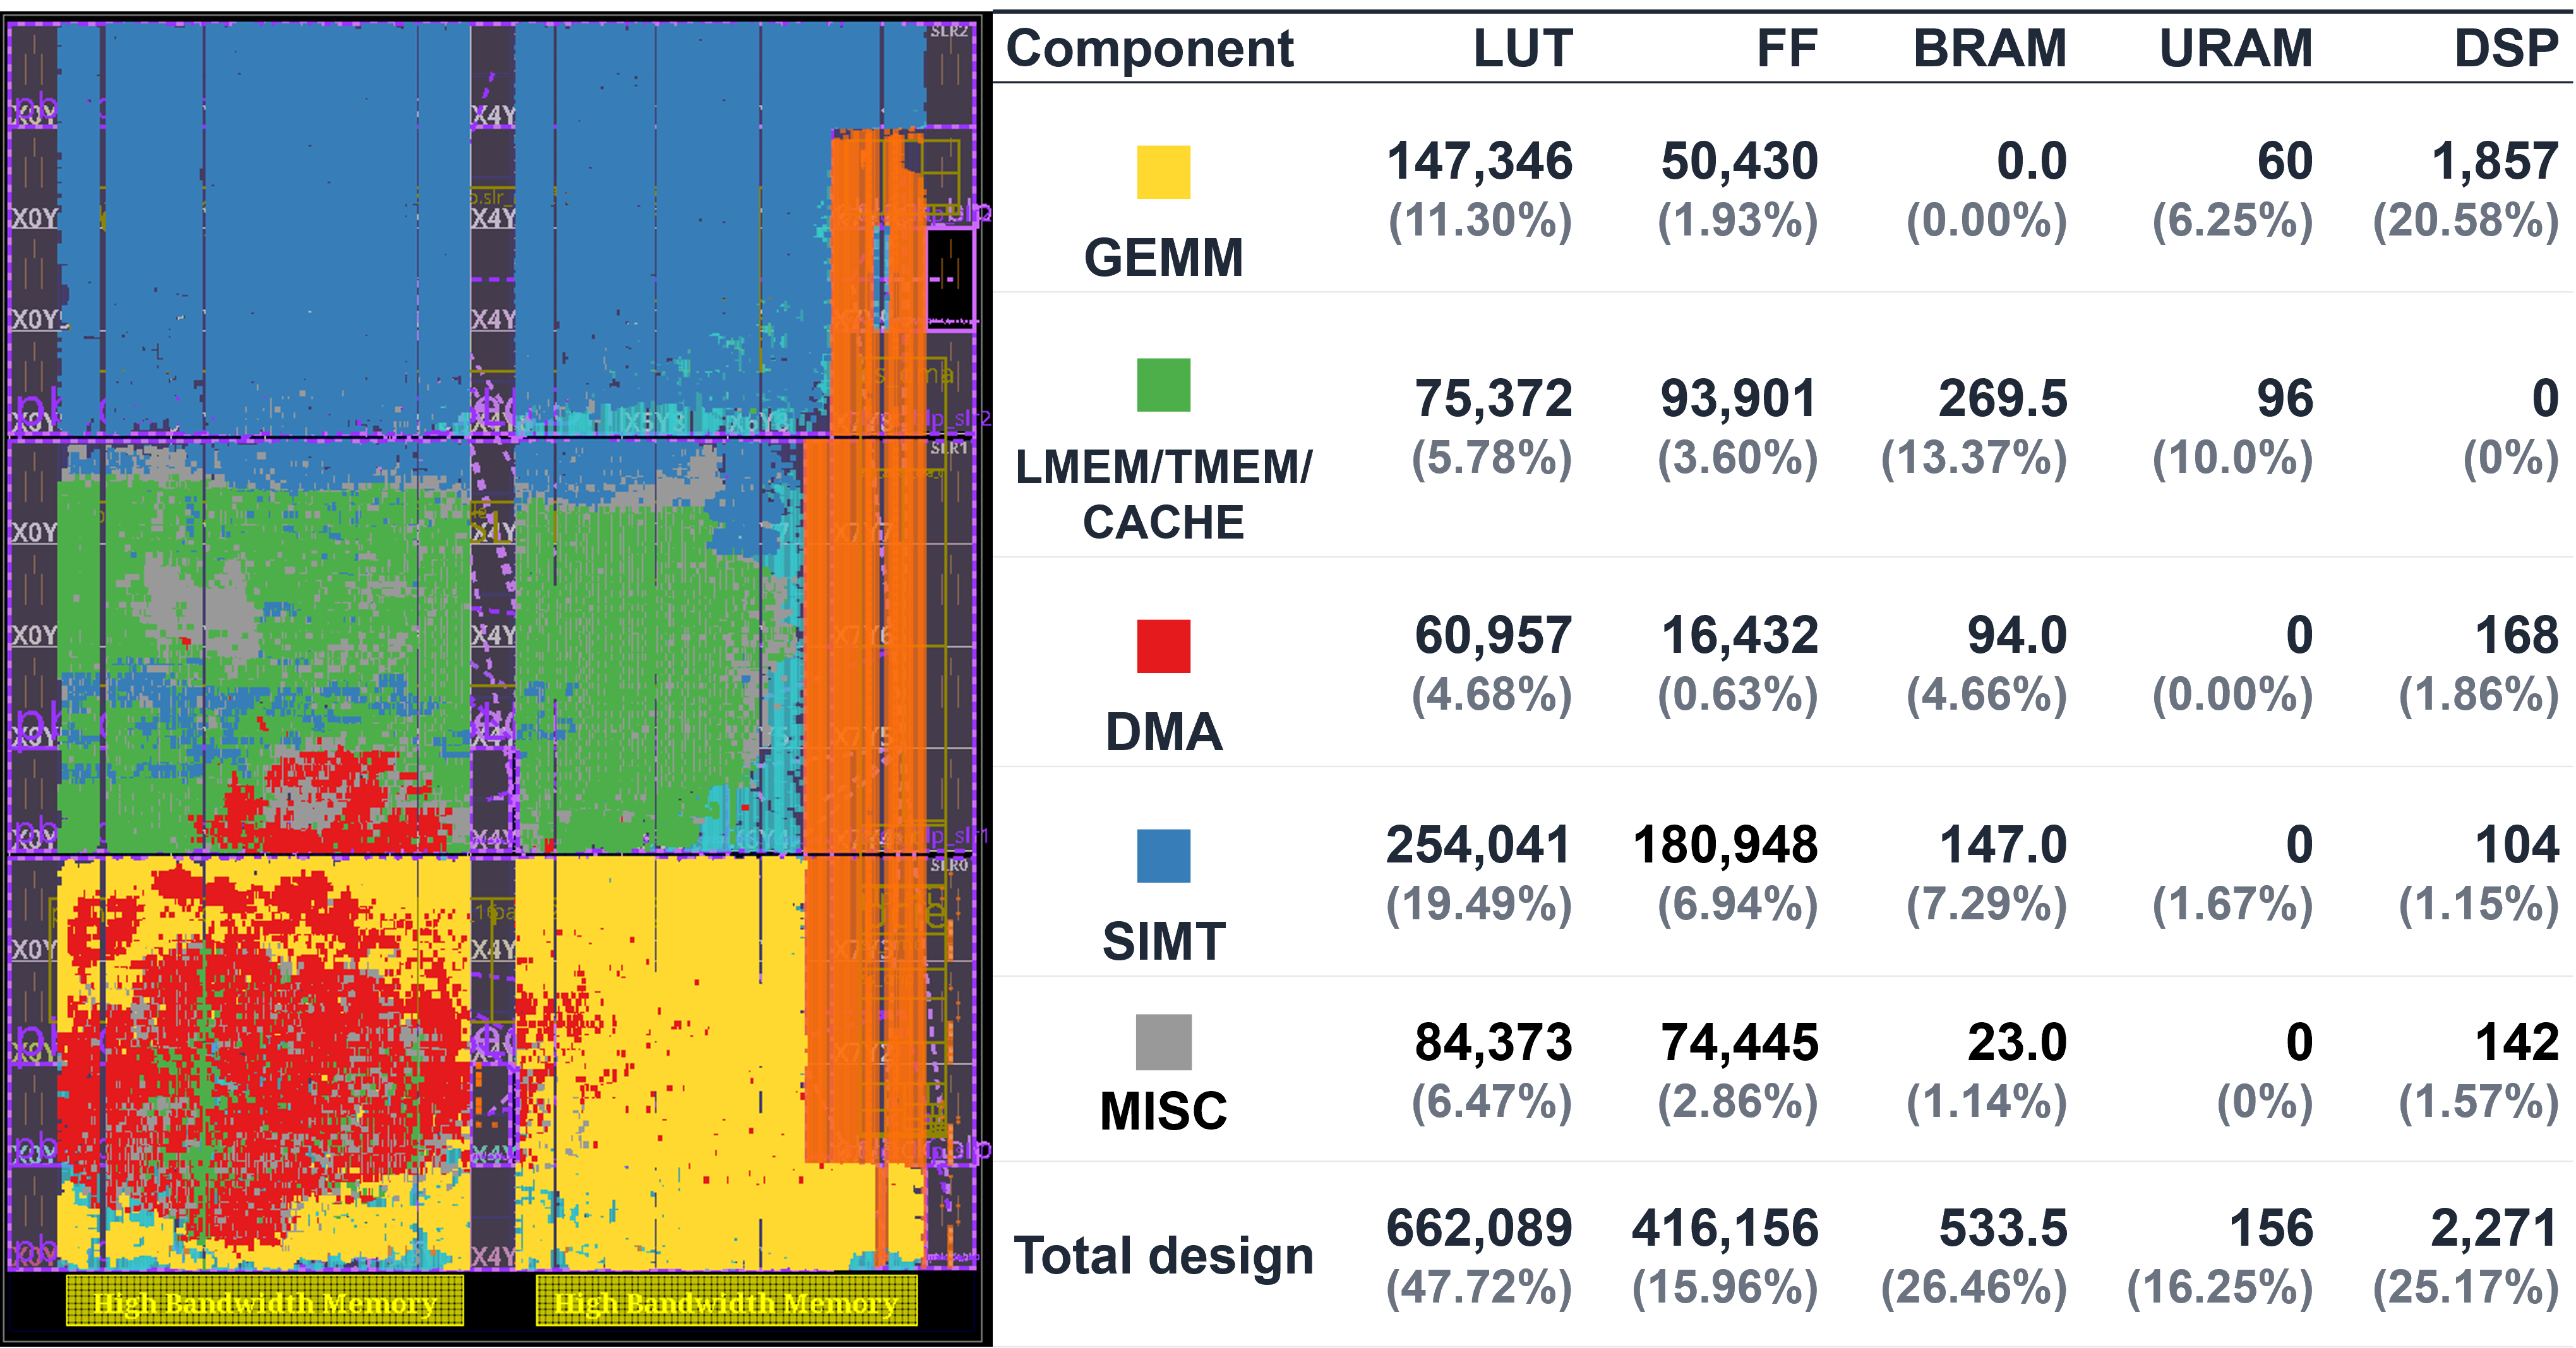
\includegraphics[width=\linewidth]{figures/floorplan.png}
    \caption{Floorplan and resource breakdown of \Cfou{} on the Alveo U55C.}
    \label{fig:floorplan}
\end{figure}

Table~\ref{tab:candidates} lists the candidate parameters. All candidates use one core with 4 warps per core and 32 threads per warp. The FP TCU is 8x4x4x2, and the \fpint{} GEMM engine is a 32x32 array. Each candidate has a 32~KiB L1 instruction cache, and a 32~KiB L1 data cache for a total cache capacity of 32~KiB. When tensor memory is present, the combined local-memory and tensor-memory capacity equals the local-memory capacity of the other candidates.

All latency results come from placed-and-routed designs deployed on a Xilinx
Alveo U55C FPGA at 100\,MHz. Figure~\ref{fig:floorplan} shows the floorplan and
resource breakdown of the final design. Each candidate runs the same \wkv{}
quantized model and differs only in its hardware mapping. For area
normalization, the candidate designs are synthesized using Synopsys Design
Compiler targeting 100\,MHz in a 28\,nm technology node. The candidate-specific
area includes the FP TCU, the \fpint{} GEMM engine, the DMA engines, and
interconnect control logic, including arbitration. We exclude the common SIMT
datapath and the on-chip SRAM area because the SIMT organization and aggregate
on-chip SRAM capacity are identical across all candidates. For candidate $i$,
we first compute the area--latency product $P_i=L_iA_i$, where $L_i$ and $A_i$
are its measured FPGA latency and candidate-specific synthesized area,
respectively. For each workload, we report the relative area-normalized latency
$P_i/\min_j P_j=(L_iA_i)/\min_j(L_jA_j)$ over candidates
$j\in\{\mathrm{C1},\mathrm{C2},\mathrm{C3},\mathrm{C4}\}$, such that the
minimum value is normalized to one.

We sample total FPGA board power with \texttt{xrt-smi} during kernel execution and take the arithmetic mean of the collected samples.
We subtract the idle board power from this mean to obtain the kernel's dynamic power.
When a kernel runs too briefly to collect enough power samples, we wrap its body in a loop and execute multiple iterations during measurement.
We compute each kernel's energy from its dynamic power and measured latency, and obtain end-to-end latency and energy by summing the corresponding per-kernel values.
The reported energy per token is the total end-to-end energy divided by the number of processed tokens.

\begin{table}[t]
\centering
\caption{Hardware candidates for evaluation.}
\label{tab:candidates}

\scriptsize
\setlength{\tabcolsep}{1pt}

\begin{tabular*}{\columnwidth}{@{\extracolsep{\fill}}*{10}{c}@{}}
  \toprule                                                                                                                                          
  ID
  & \shortstack{Cores}
  & \shortstack{Warps}
  & \shortstack{Threads}
  & \shortstack{FP TCU}
  & \shortstack{\fpint{}\\MXU}
  & \shortstack{Cache}
  & \shortstack{LMEM}
  & \shortstack{TMEM}
  & \shortstack{ACC\\MEM} \\
  \midrule
  C1 & 1 & 4 & 32 & 8x4x4x2 & --    & 32K & 1M & -- & -- \\
  C2 & 1 & 4 & 32 & 8x4x4x2 & 32x32 & 32K & 1M & -- & -- \\
  C3 & 1 & 4 & 32 & --      & 32x32 & 32K & 768K & -- & 256K \\
  C4 & 1 & 4 & 32 & --      & 32x32 & 32K & 512K & 256K & 256K \\
  \bottomrule
  \end{tabular*}
\end{table}

\textbf{Workloads.}
The evaluation covers prefill, decode, and end-to-end inference. 
The workloads are Llama2-7B and Llama3-8B, quantized with SpinQuant to 4-bit weights and KV.
We include all vector kernels used by SpinQuant, including the Hadamard transform.
GEMM operations execute on the FP TCU and/or \fpint{} GEMM engine available in each candidate.
In C4, vector kernels adjacent to GEMM operations fuse the layout
transformation to avoid a separate transformation pass.
% The quantization options follow the default parameters of SpinQuant.

\textbf{Software Implementation.}
The kernel launch code uses the Vortex runtime, and kernels are implemented natively in C++ for Vortex. 
Vector operations follow an SPMD style, while GEMM operations use either the Vortex FP TCU kernels or the \fpint{} MXU through MMIO-programmed GEMM descriptors. 
A kernel writes the matrix size, quantized input transpose flag, quantization direction, and related metadata, invokes the GEMM node, and polls an MMIO status register until completion. 
Execution order, descriptor setup, and layout handling are expressed directly in the native kernels and runtime code.
We use the same sequential kernel execution model for all candidates.
The $QK^T$ GEMM completes and writes the attention score tensor to HBM before a separate Vortex SIMD kernel reads it and computes online softmax.
The softmax output is then written back to HBM and consumed by the following PV GEMM kernel.
Online softmax therefore refers to the algorithm used inside the standalone SIMD kernel.
We do not fuse $QK^T$, softmax, and PV into a single tiled attention kernel.
The reported latency and energy include these kernels and their intermediate HBM transfers.
This common execution model ensures that all candidates use the same attention schedule while differing in the GEMM datapath and memory system.
This implementation evaluates \ours{} inside an LLM inference flow rather than as a bare GEMM microbenchmark, so the memory system, runtime layout, and native \fpint{} attention support operate together.

\subsection{GEMM-Only Latency}

We first isolate the GEMM portion of inference to identify how each architectural
step affects the compute and memory paths that feed the MXU. The GEMM-only
results sum the Q/K/V/O projections, the $QK^T$ and PV attention GEMMs, and the
FFN projections, while excluding vector kernels and fused layout
transformations. Within each workload, the minimum candidate value is
normalized to one.

Across the latency results, the candidate sequence provides three controlled comparisons:
C1--C2 tests whether linear-only \fpint{} acceleration is sufficient;
C2--C3 isolates the benefit of executing attention on the native \fpint{}
datapath; and C3--C4 isolates the benefit of the optimized memory, layout, and
runtime system. The raw GEMM latency result below establishes this progression;
the subsequent latency results examine area normalization and end-to-end overheads.

\begin{figure}[t]
    \centering
    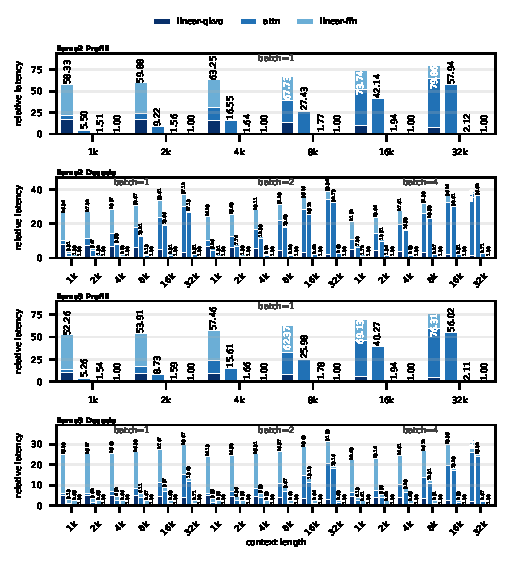
\includegraphics[width=\columnwidth]{figures/llama2_3/figures_script/llama_gemm_only_no_area_norm/llama_gemm_only_latency_no_area_norm.pdf}
    \caption{GEMM-only relative latency without area normalization. Within each
    workload, the four bars from left to right represent C1--C4, with the
    minimum candidate value normalized to one. Colors group the Q/K/V/O
    projections, the $QK^T$ and PV attention GEMMs, and the FFN projections.}
    \label{fig:gemm-latency-no-area-norm}
\end{figure}

\textbf{Latency without area normalization.}
Figure~\ref{fig:gemm-latency-no-area-norm} first compares the measured FPGA
latency without accounting for candidate area. C4 reduces GEMM latency over C1
by $63.97\times$ on geomean in prefill and $28.20\times$ in decode. C2 reduces
latency over C1 by $3.35\times$ and $2.74\times$, respectively, by moving the
linear projections to the larger \fpint{} MXU, but leaves $QK^T$ and PV on the
FP TCU. C3 removes this attention fallback and reduces latency over C2 by
$10.91\times$ and $4.37\times$. Finally, C4 reduces latency over C3 by another
$1.75\times$ and $2.35\times$ while retaining the same \fpint{} arithmetic
coverage.

These comparisons identify two successive bottlenecks: the FP attention
fallback and the general-purpose operand-delivery path. Native \fpint{}
attention removes the former, while C4's aligned tile-major accesses, increased
TMEM bank parallelism, and higher-bandwidth HBM--TMEM path remove the latter.

\begin{figure}[t]
    \centering
    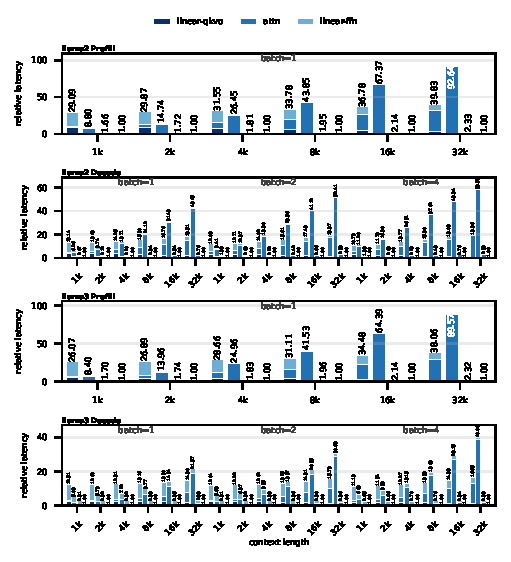
\includegraphics[width=\columnwidth]{figures/llama2_3/figures_script/llama_gemm_only/llama_gemm_only_latency.pdf}
    \caption{Area-normalized GEMM-only relative latency. Within each workload,
    the four bars from left to right represent C1--C4, with the minimum
    candidate value normalized to one. Colors group the Q/K/V/O projections,
    the $QK^T$ and PV attention GEMMs, and the FFN projections.}
    \label{fig:gemm-latency-area-norm}
\end{figure}

\textbf{Area-normalized latency.}
Figure~\ref{fig:gemm-latency-area-norm} accounts for the synthesized area of
each candidate. C4 reduces area-normalized GEMM latency over C1 by
$31.91\times$ on geomean in prefill and $14.06\times$ in decode. The main
effect of area normalization is to expose the cost of C2's two compute units:
although C2 improves raw latency in every case, it only nearly
matches C1 on geomean in prefill, with a $1.04\times$ reduction, and has
$1.17\times$ higher latency than C1 in decode. C2 is slower than C1 in half of
the prefill cases and in 22 of the 36 decode cases. C3 and C4 then preserve the
raw-latency ordering: C3 reduces the metric over C2 by $15.85\times$ and
$6.35\times$, and C4 further reduces it by $1.93\times$ and $2.59\times$.
Thus, the optimized tensor path recovers more performance than its added area.

\subsection{End-to-End Latency and Layout Overhead}

We next include the complete inference path: all GEMMs, all non-GEMM vector
kernels, fused layout transformations, and intermediate HBM transfers. The
breakdowns separate these costs into \emph{gemm}, \emph{layout}, and
\emph{vector}. The layout portion is the incremental overhead of producing or
consuming tile-major tensors inside the adjacent fused vector kernels, whereas
the vector portion contains the remaining non-GEMM work.

\begin{figure}[t]
    \centering
    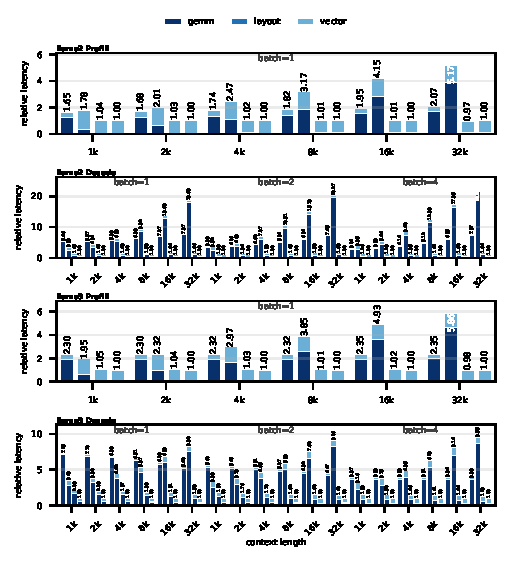
\includegraphics[width=\columnwidth]{figures/llama2_3/figures_script/llama_e2e_gemm_layout_vector_stacked/llama_e2e_gemm_layout_vector_latency_stacked.pdf}
    \caption{Area-normalized end-to-end relative latency, decomposed into GEMM,
    fused layout-transformation overhead, and the remaining vector kernels.
    Within each workload, the four bars from left to right represent C1--C4,
    with the minimum candidate value normalized to one.}
    \label{fig:e2e-latency-gemm-layout-vector}
\end{figure}

\textbf{End-to-end latency and layout overhead.}
Figure~\ref{fig:e2e-latency-gemm-layout-vector} shows that C4 reduces
area-normalized end-to-end latency over C1 by $2.05\times$ on geomean in
prefill and $5.20\times$ in decode, with maximum improvements of
$2.35\times$ and $7.87\times$, respectively. The same candidate progression
remains visible: C2 is slower than C1, C3 removes the FP attention fallback,
and C4 provides the lowest latency.

The gap between GEMM-only and end-to-end improvements reflects the inclusion of
the common vector kernels: the C4-over-C3 improvement is $1.02\times$ in
prefill and $1.55\times$ in decode. Decode retains more of the GEMM-path
improvement because non-GEMM vector kernels account for a smaller fraction of
its end-to-end latency. The explicit layout segment remains limited across the
evaluated workloads, showing that C4 retains its end-to-end benefit after accounting
for fused tile-major conversion.

\subsection{Dynamic Power and Energy}

\textbf{Dynamic power.}
Table~\ref{tab:kernel-dynamic-power} first summarizes the idle-subtracted
dynamic board power used in the energy calculation. Each entry reports the
mean and standard deviation across the measured invocations. The three GEMM
paths span 1.76--2.31~W: the optimized \fpint{} GEMM draws 2.00~W, compared
with 2.31~W for its naive counterpart and 1.76~W for the FP TCU. These power
differences are substantially smaller than the corresponding latency
differences, so execution time remains the dominant source of the candidate
energy differences.

\begin{table}[t]
    \centering
    \caption{Idle-subtracted kernel dynamic board power (mean $\pm$
    standard deviation), in watts.}
    \label{tab:kernel-dynamic-power}
    \scriptsize
    \setlength{\tabcolsep}{2.5pt}
    \begin{tabular*}{\columnwidth}{@{\extracolsep{\fill}}lrlr@{}}
        \toprule
        Kernel & Power & Kernel & Power \\
        \midrule
        Concat. & $0.89\pm0.32$ & Softmax & $2.08\pm0.35$ \\
        Elem. add & $1.67\pm0.53$ & Quant. & $1.40\pm0.71$ \\
        Elem. mul & $1.94\pm0.39$ & Dequant. & $1.23\pm0.14$ \\
        Hadamard & $1.46\pm0.83$ & FP--FP GEMM & $1.76\pm0.39$ \\
        RMSNorm & $2.11\pm0.29$ & FP--INT GEMM (naive) & $2.31\pm0.85$ \\
        RoPE & $1.10\pm0.24$ & FP--INT GEMM (opt.) & $2.00\pm0.65$ \\
        SiLU & $1.59\pm0.25$ & & \\
        \bottomrule
    \end{tabular*}
\end{table}

\textbf{End-to-end energy.}
We next evaluate whether the latency improvements translate into lower energy.
Unlike the area-normalized latency metric, kernel energy is computed from its
raw measured FPGA latency and idle-subtracted dynamic board power; no area
factor is applied. End-to-end energy sums the per-kernel energy of GEMM,
dequantization, fused layout transformation, vector execution, and intermediate
HBM transfers.

\begin{figure}[t]
    \centering
    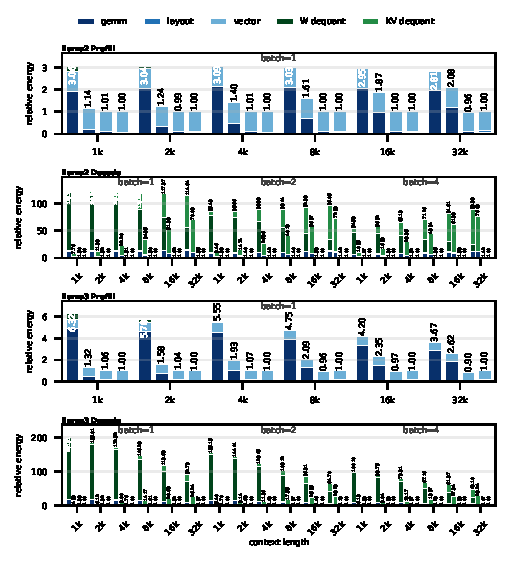
\includegraphics[width=\columnwidth]{figures/llama2_3/figures_script/llama_energy_no_area_norm_gemm_layout_vector_stacked/llama_energy_per_token_power_dynamic_avg_W_no_area_norm_gemm_layout_vector_stacked.pdf}
    \caption{End-to-end energy per token computed from raw measured FPGA
    latency and idle-subtracted dynamic board power. Within each workload, the
    four bars from left to right represent C1--C4 and the minimum candidate
    energy is normalized to one. The stacks separate GEMM, fused layout
    transformation, common vector execution, and dequantization. No area
    normalization is applied.}
    \label{fig:e2e-energy-dequant-breakdown}
\end{figure}

Figure~\ref{fig:e2e-energy-dequant-breakdown} shows that C4 reduces end-to-end
energy over C1 by $3.88\times$ on geomean in prefill, with a maximum reduction
of $6.76\times$. The corresponding geomean and maximum reductions in decode
increase to $118.97\times$ and $342.04\times$, respectively.

Prefill attention consumes the K and V values produced for the current prompt
directly, while their quantized copies are retained for subsequent decode.
Prefill therefore requires no KV-cache dequantization. The dequantization
segment visible for C1 in prefill consists only of static 4-bit weight
dequantization; C2--C4 execute their linear layers on the native \fpint{} MXU.

Decode exhibits a different behavior. Although each step produces only one new
token, its $QK^T$ and PV operations consume the K and V elements accumulated
over the entire preceding context. C1 and C2 execute these attention GEMMs on
the FP TCU and thus dequantize all consumed KV-cache elements at every step.
Across the decode workloads, dequantization accounts for an average of 90.3\%
and 79.2\% of the total energy of C1 and C2, respectively. C1 includes both
static-weight and KV-cache dequantization, whereas C2's dequantization segment
is solely the KV-cache conversion.

C2 therefore isolates the attention-side cost: it already executes the linear
projections on the native \fpint{} MXU but retains FP TCU execution for $QK^T$
and PV. Consequently, C2 consumes $14.45\times$ more decode energy than C3 on
geomean, and up to $53.06\times$ more. C3 and C4 eliminate this repeated
conversion by consuming quantized K and V operands directly in the native
\fpint{} attention path. Thus, linear-only \fpint{} acceleration is
insufficient to realize the decode-energy benefit of WKV quantization.

\begin{comment}
\subsection{End-to-End Performance Improvement}

% \begin{figure}[!t]
%     \centering

%     \begin{subfigure}[t]{\linewidth}
%         \centering
%         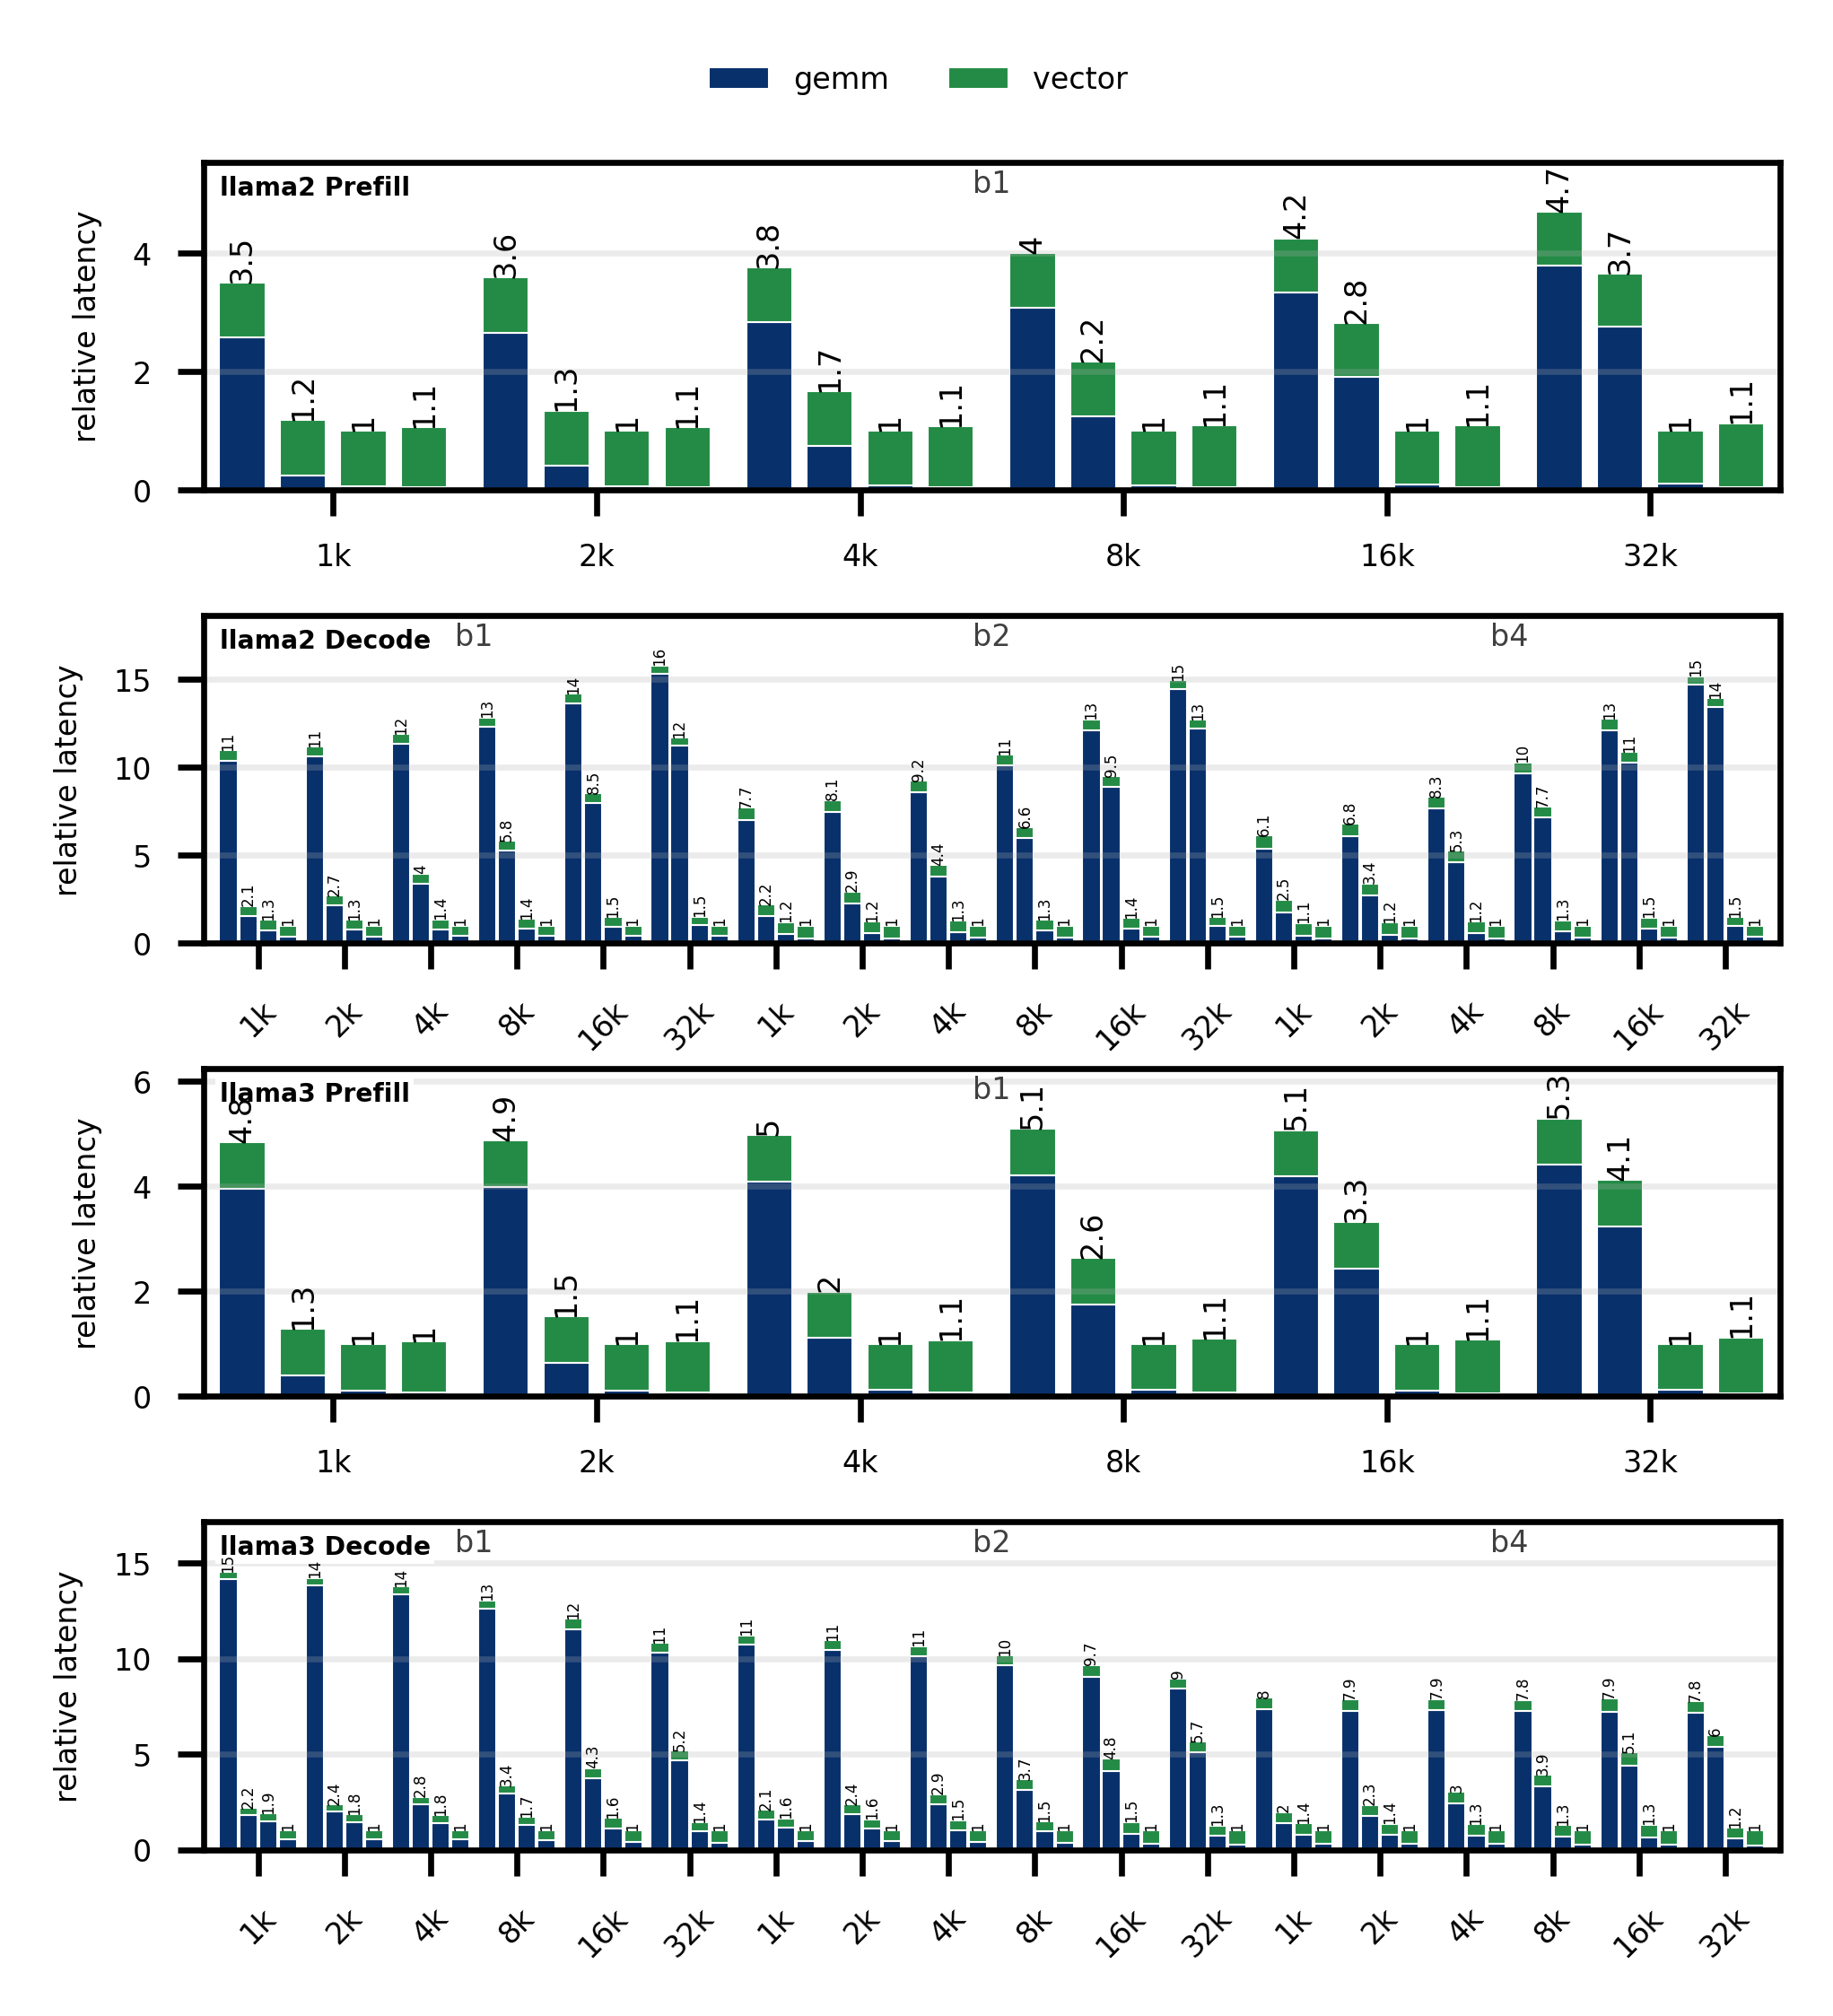
\includegraphics[width=0.92\linewidth]{figures/llama2_3/figures_script/llama_e2e_no_area_norm_stacked/llama_e2e_latency_no_area_norm_stacked.png}
%         \caption{Without area normalization.}
%         \label{fig:e2e-latency-no-area-norm}
%     \end{subfigure}

%     \vspace{0.3em}

%     \begin{subfigure}[t]{\linewidth}
%         \centering
%         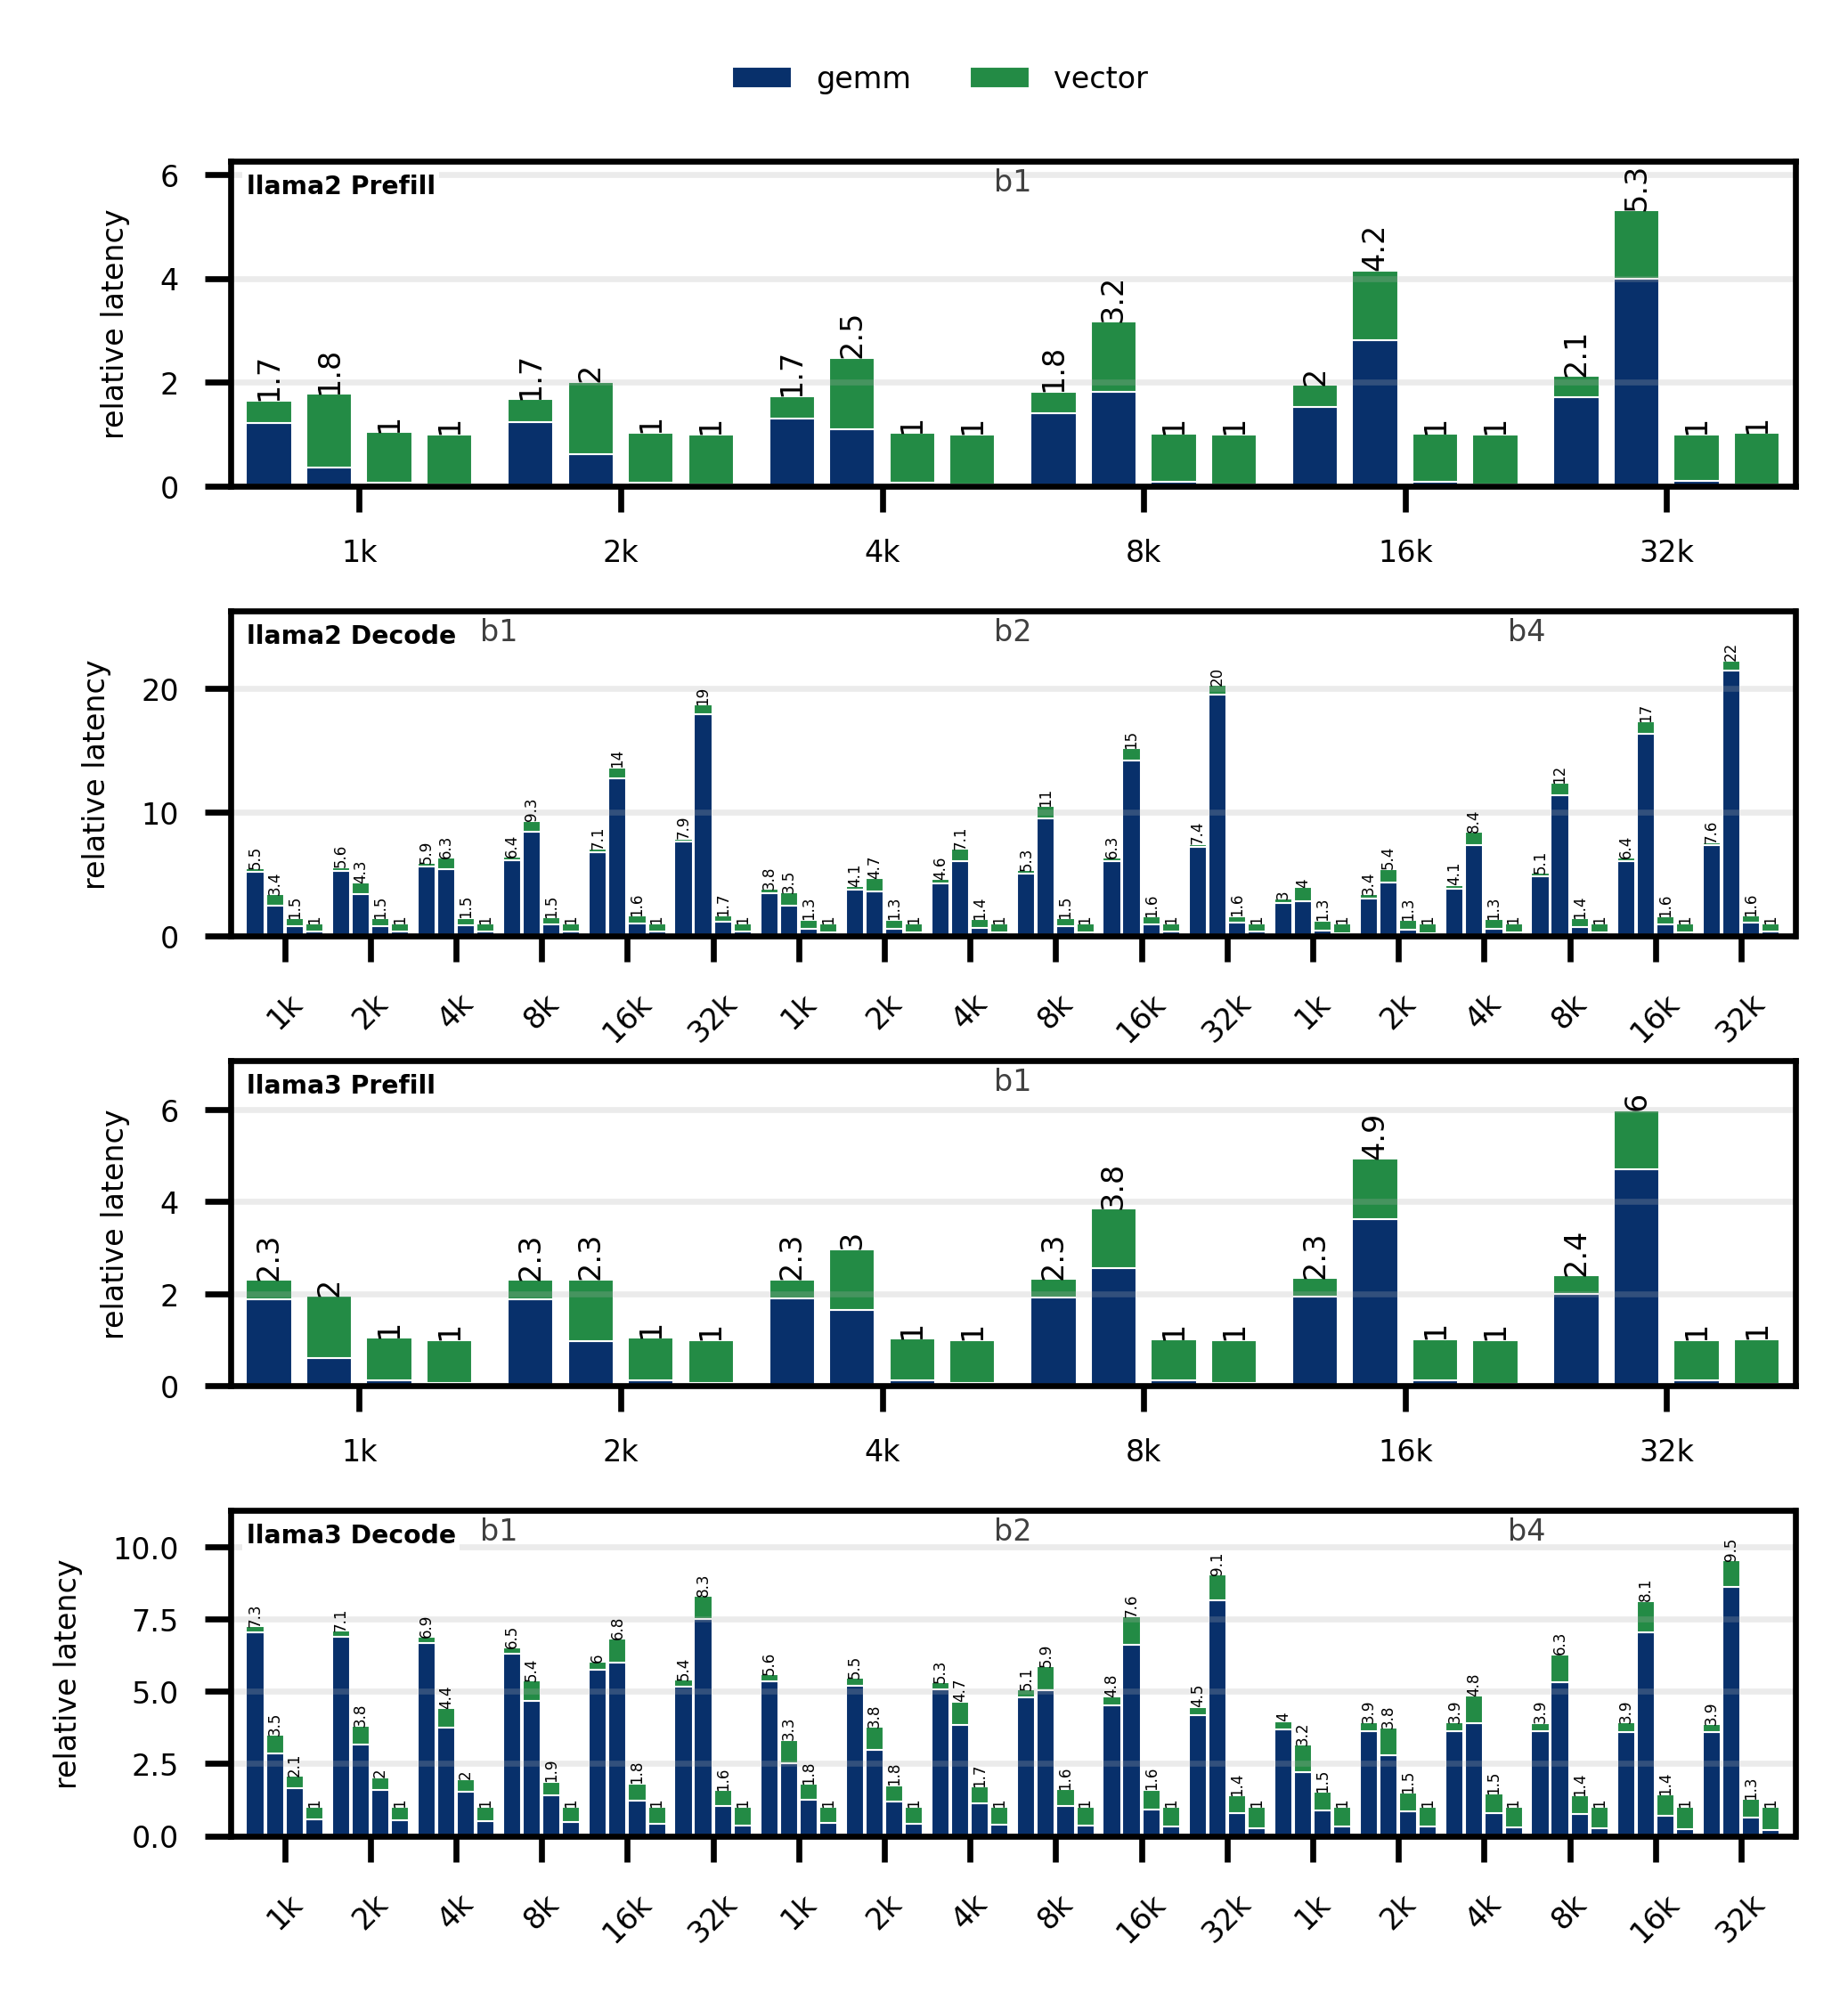
\includegraphics[width=0.92\linewidth]{figures/llama2_3/figures_script/llama_e2e_stacked/llama_e2e_latency_stacked.png}
%         \caption{With area normalization.}
%         \label{fig:e2e-latency-area-norm}
%     \end{subfigure}

%     \caption{End-to-end relative latency of Llama2-7B and Llama3-8B W4A16KV4 inference (a) without and (b) with area normalization. Within each workload, the four bars from left to right represent C1--C4 and are normalized to C4. The vector portion includes all non-GEMM kernels, including fused layout transformations.}
%     \label{fig:e2e-latency-stacked}
% \end{figure}
\begin{figure*}[!t]
    \centering

    \begin{subfigure}[t]{0.49\textwidth}
        \centering
        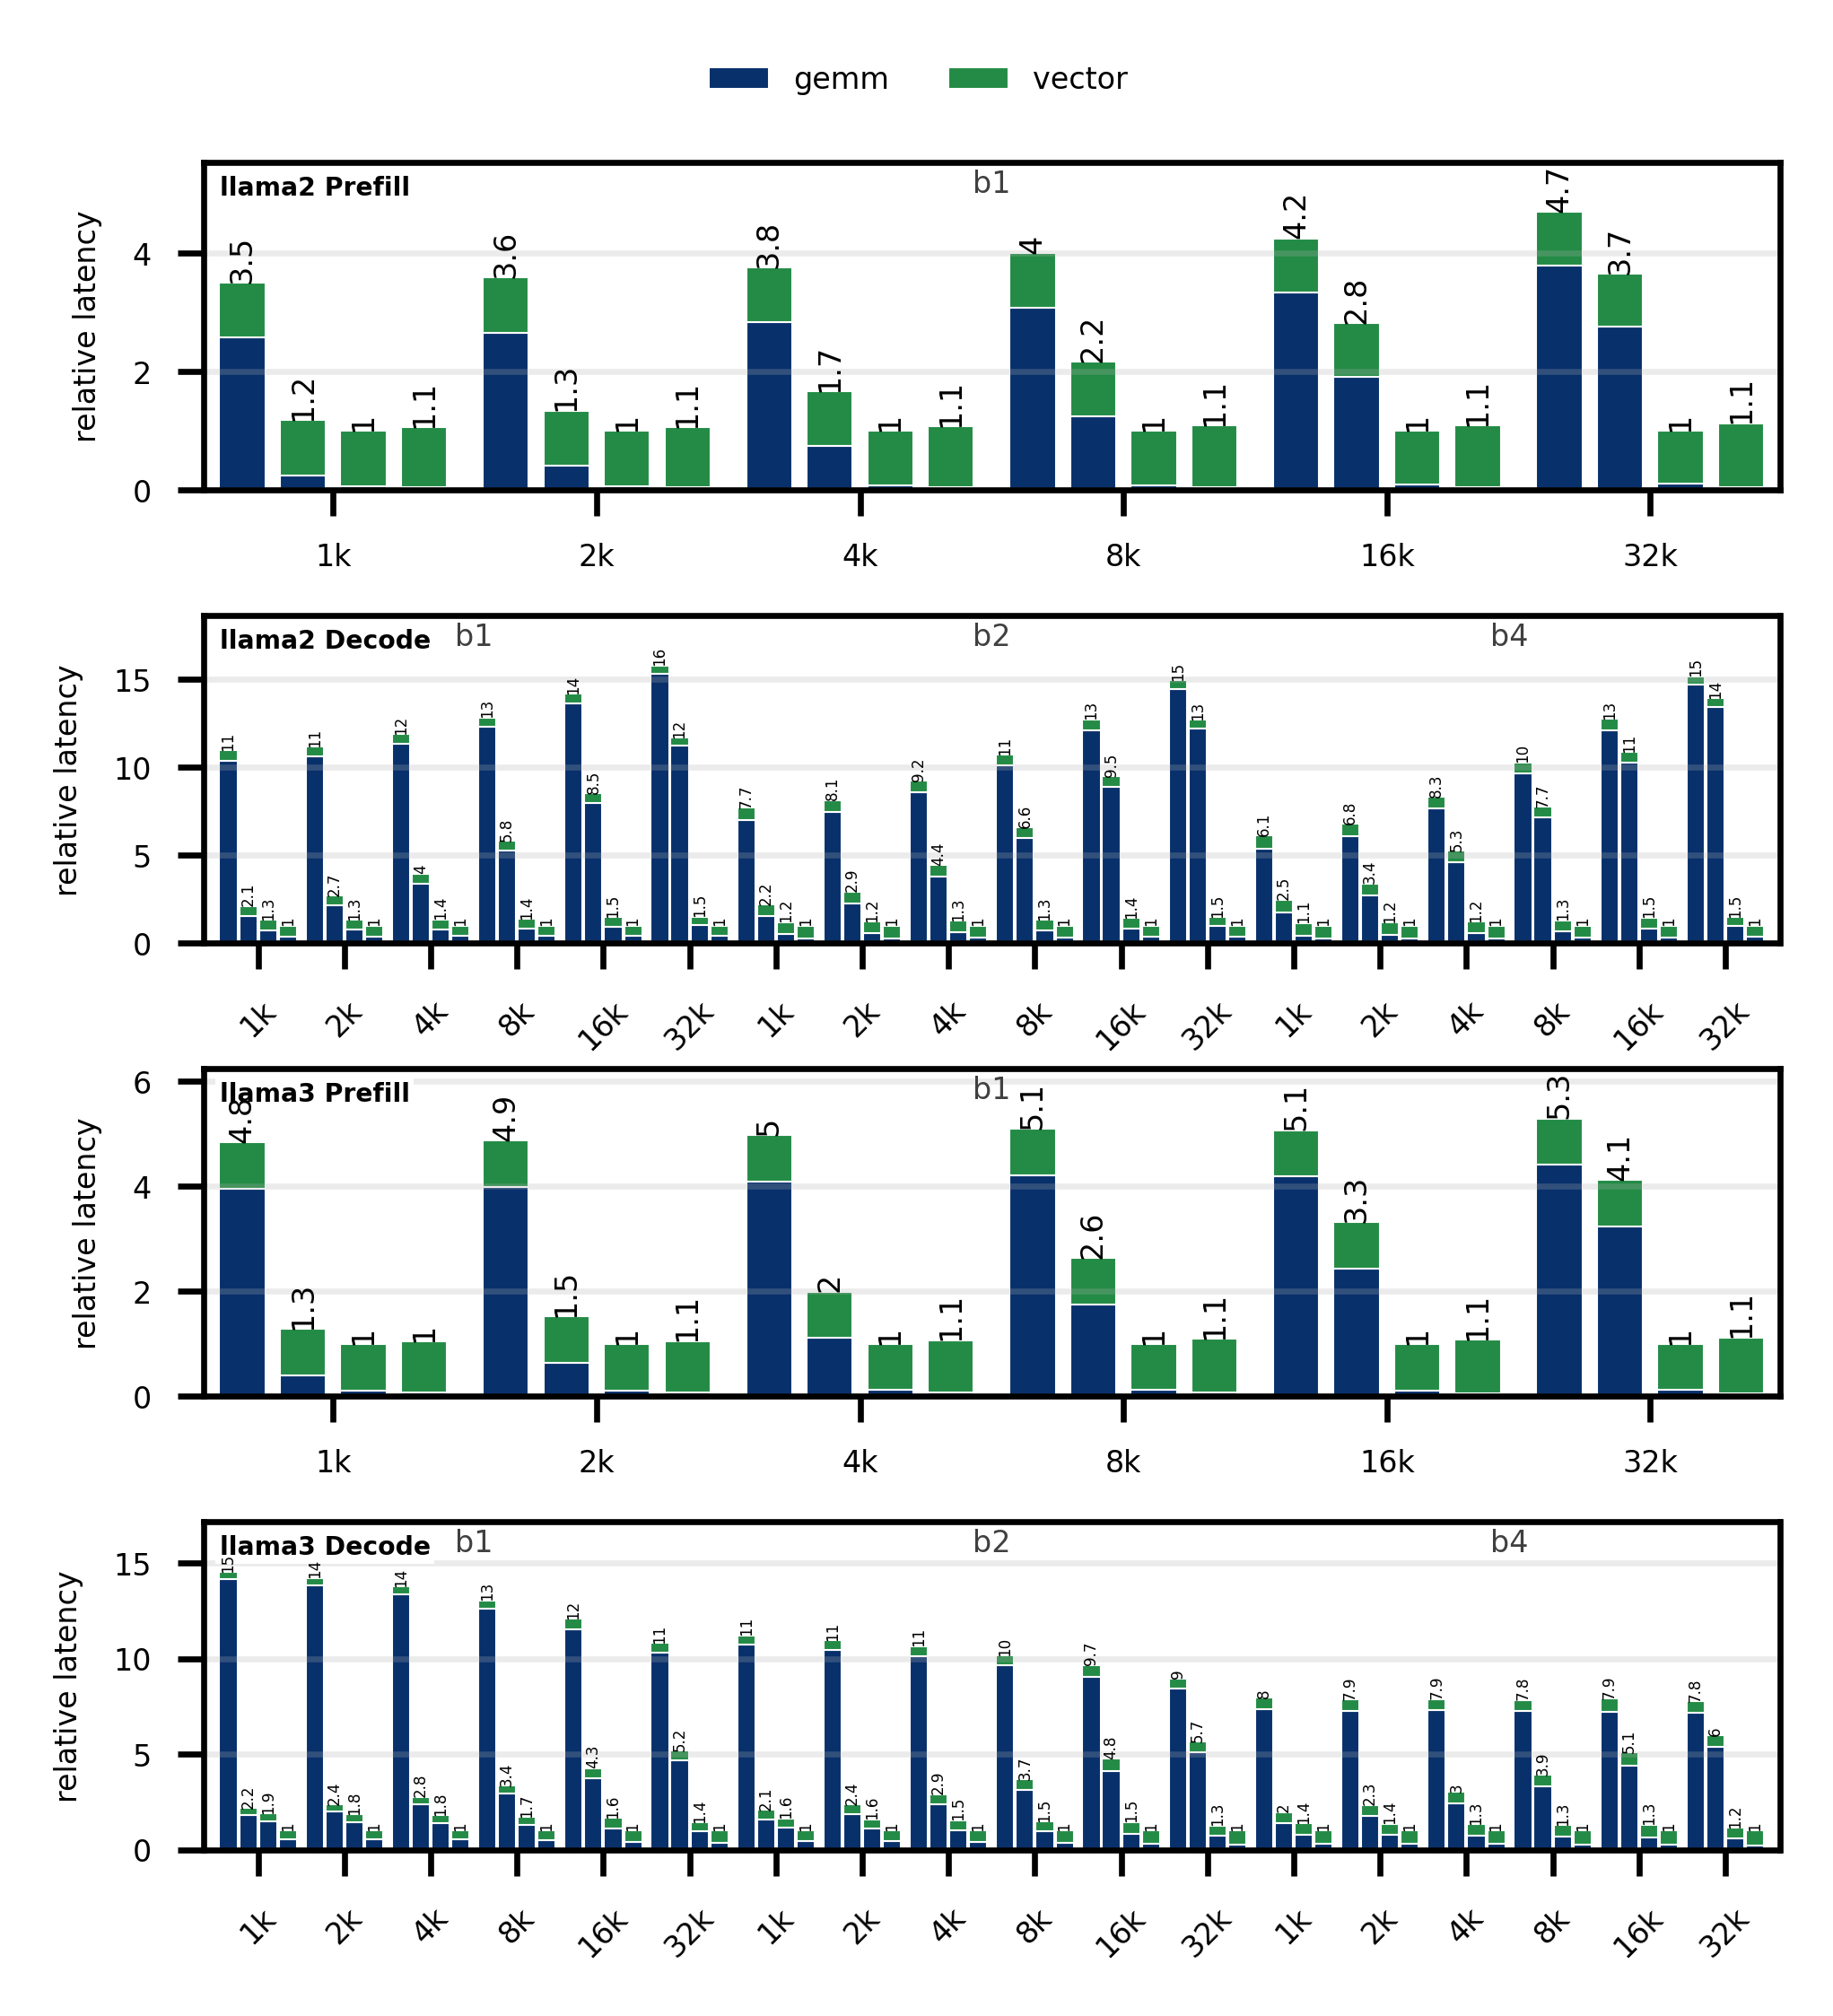
\includegraphics[width=0.92\linewidth]{figures/llama2_3/figures_script/llama_e2e_no_area_norm_stacked/llama_e2e_latency_no_area_norm_stacked.png}
        \caption{Without area normalization.}
        \label{fig:e2e-latency-no-area-norm}
    \end{subfigure}
    \hfill
    \begin{subfigure}[t]{0.49\textwidth}
        \centering
        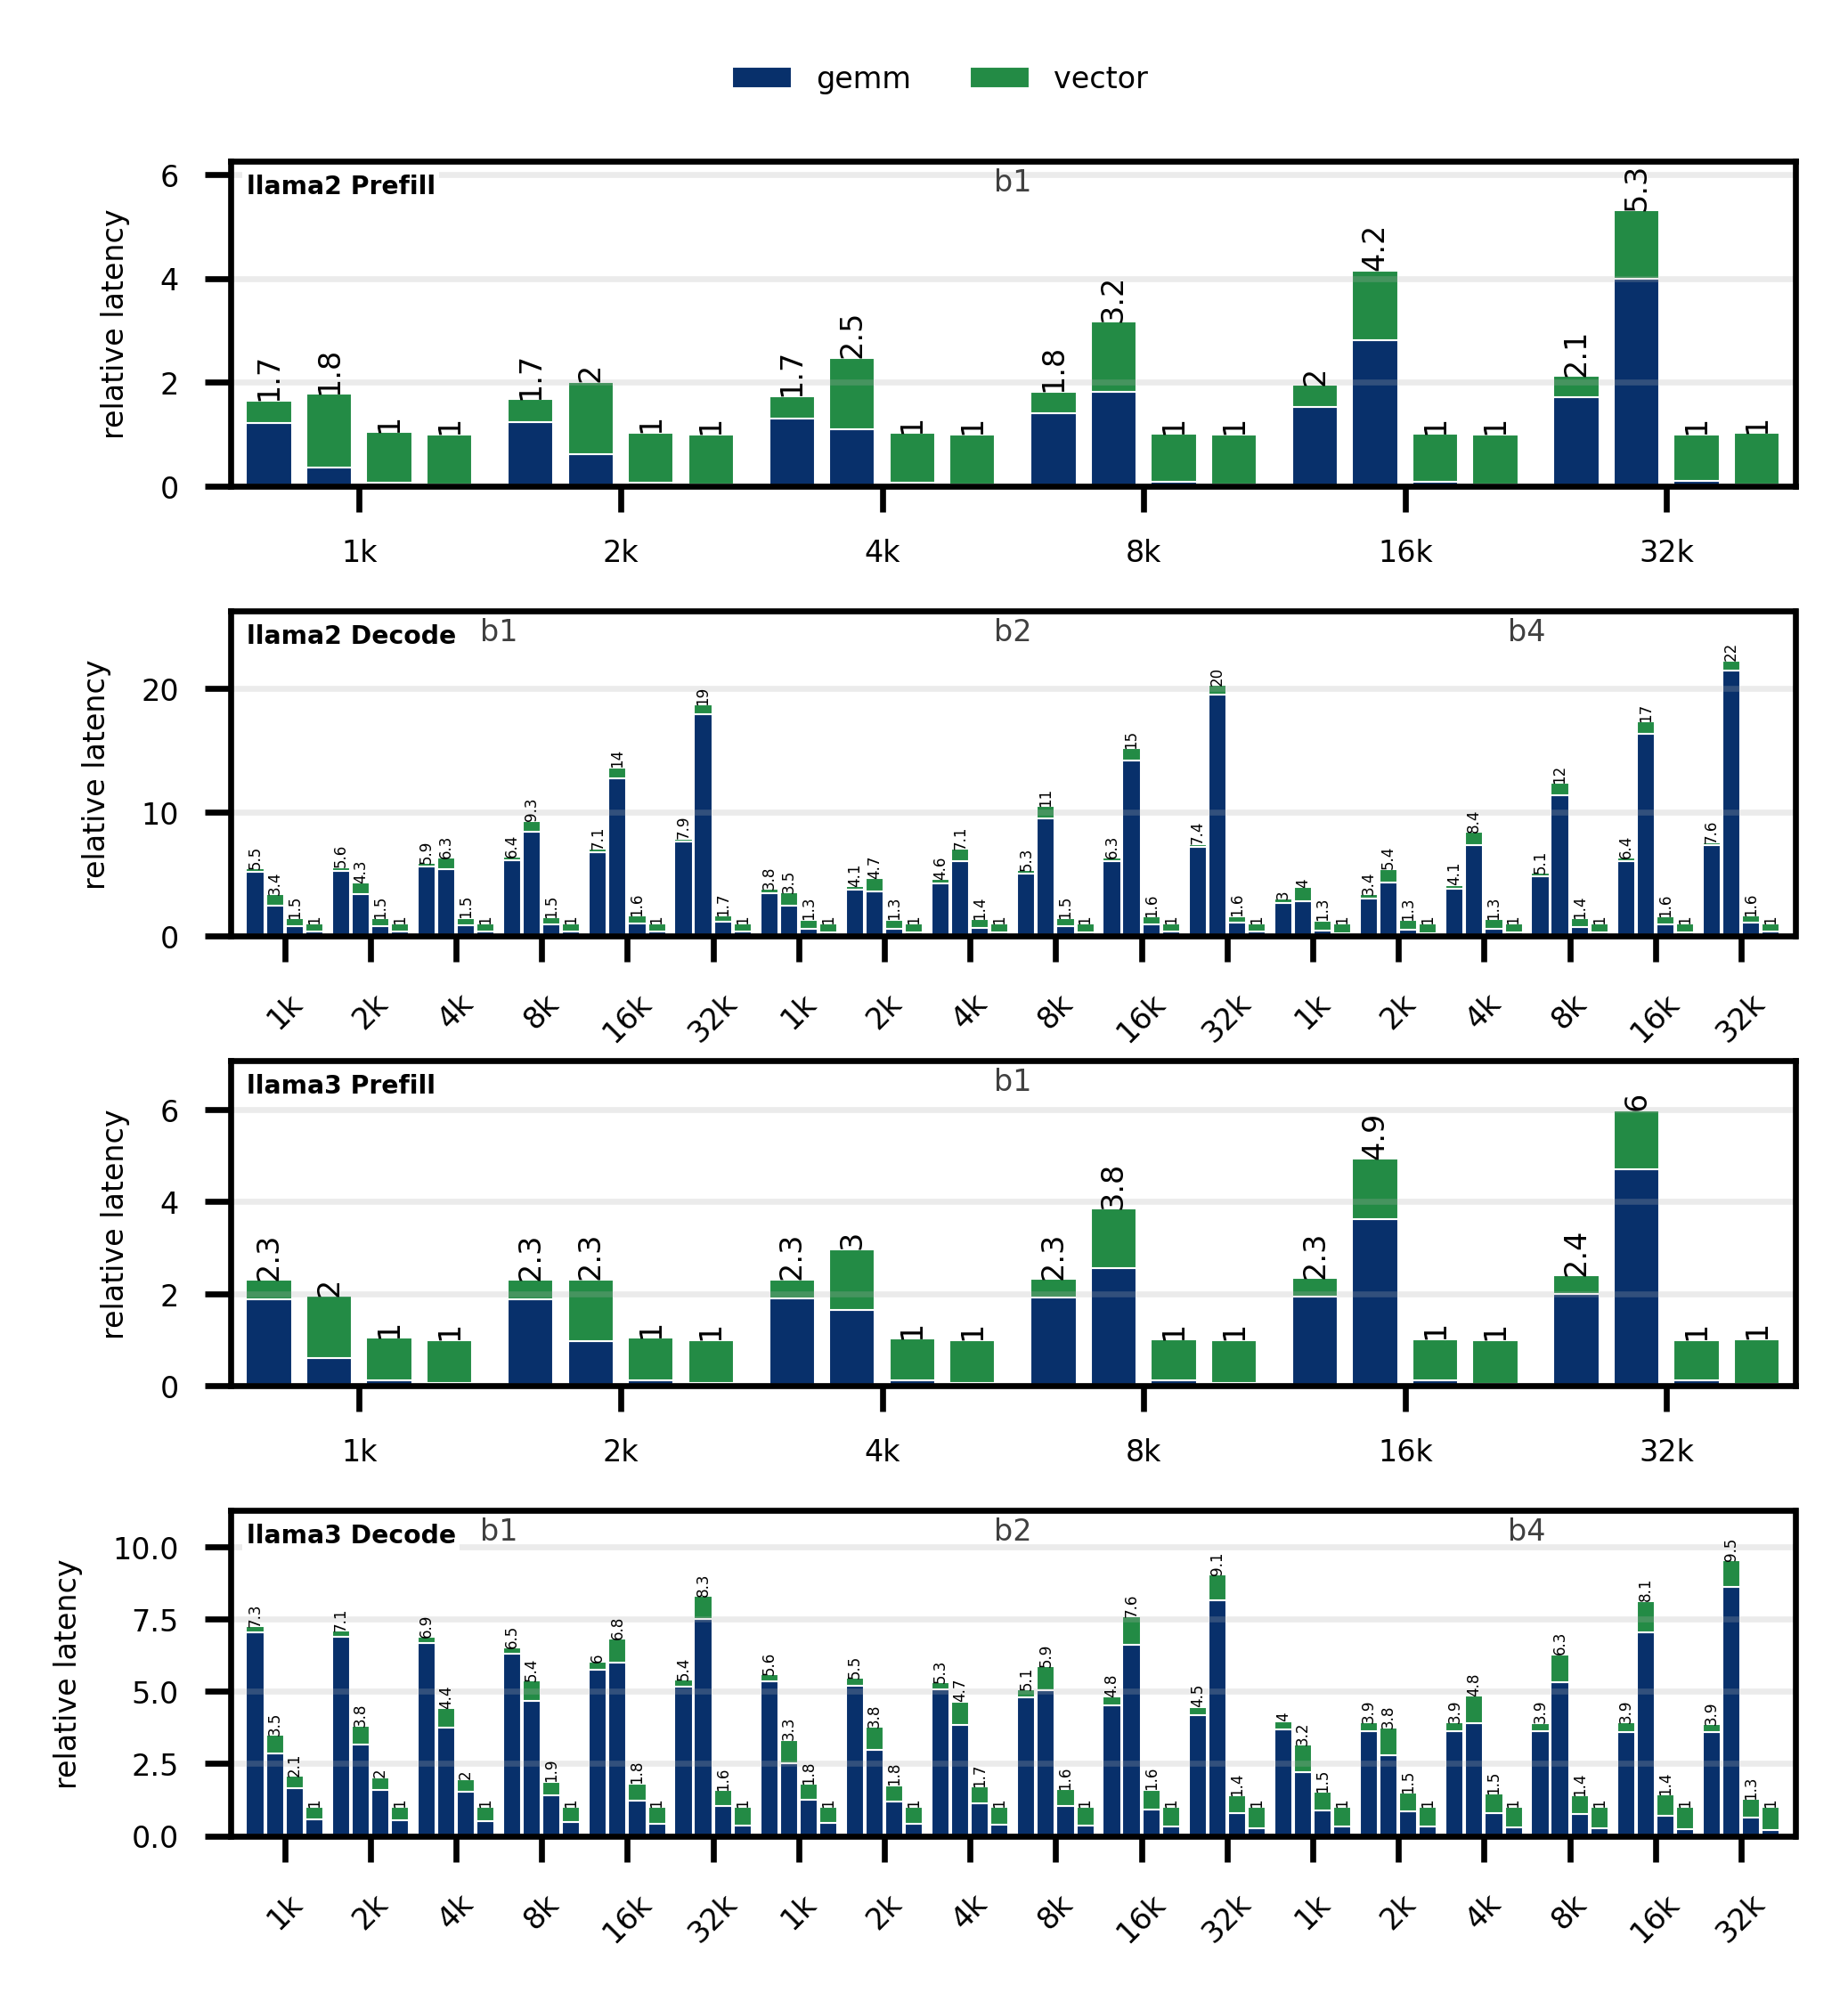
\includegraphics[width=0.92\linewidth]{figures/llama2_3/figures_script/llama_e2e_stacked/llama_e2e_latency_stacked.png}
        \caption{With area normalization.}
        \label{fig:e2e-latency-area-norm}
    \end{subfigure}

    \caption{End-to-end relative latency of Llama2-7B and Llama3-8B
    W4A16KV4 inference (a) without and (b) with area normalization.
    Within each workload, the four bars from left to right represent
    C1--C4 and are normalized to C4. The vector portion includes all
    non-GEMM kernels, including fused layout transformations.}
    \label{fig:e2e-latency-stacked}
\end{figure*}

Figure~\ref{fig:e2e-latency-stacked} compares the end-to-end latency of C1--C4 without and with area normalization when running Llama2-7B and Llama3-8B inference with 4-bit weight and KV-cache quantization.
We evaluate prefill at batch size 1 and decode at batch sizes 1, 2, and 4, with sequence lengths ranging from 1k to 32k.
In the area-normalized results in Figure~\ref{fig:e2e-latency-area-norm}, \Cfou{} reduces latency over the FP TCU baseline by $3.24\times$ on geomean in prefill
and $4.73\times$ on geomean in decode, with maximum improvements of $4.31\times$ and $7.96\times$, respectively.

Comparing C1 and C2 shows why a linear-only \fpint{} accelerator is insufficient. 
C2 accelerates the linear projections, but it still executes $QK^T$ and PV on the FP TCU while carrying the area cost of both the FP TCU and the \fpint{} MXU.
Consequently, C2's geomean latency is $1.30\times$ that of C1 in prefill and $1.94\times$ that of C1 in decode.
C2 is slower than C1 in 8 of the 12 prefill cases and in all 36 decode cases.
These results demonstrate that accelerating only the linear layers does not preserve the array-level efficiency advantage at the system level when attention remains on the FP datapath.

C3 routes both the linear layers and the $QK^T$ and PV GEMMs through the \fpint{} path, eliminating the FP attention fallback.
This change reduces geomean latency over C2 by $2.31\times$ in prefill and $2.20\times$ in decode, demonstrating the importance of supporting attention on the same \fpint{} datapath as the linear layers.

C4 further reduces geomean latency over C3 by $1.83\times$ in prefill and $4.18\times$ in decode.
The larger decode improvement shows that native \fpint{} attention is not sufficient by itself: the MXU must be paired with a memory subsystem and runtime that sustain tensor bandwidth.
The direct tensor path, tensor memory, DMA, and layout-aware runtime reduce the cost of supplying operands and moving KV-cache data, allowing the larger MXU to translate its array-level advantage into end-to-end performance.

% \begin{figure}[t]
%     \centering
%     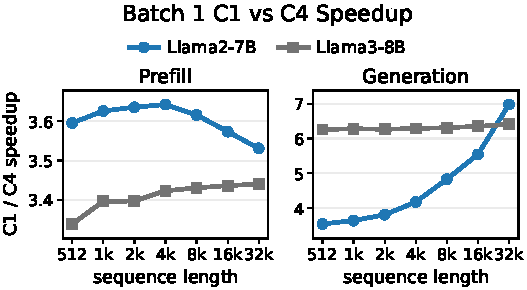
\includegraphics[width=\linewidth]{figures/llama2_3_compare/c1_vs_c4_speedup_batch1.pdf}
%     \caption{C4 speedup over C1 at batch size 1 across sequence length for Llama2-7B and Llama3-8B.}
%     \label{fig:llama3_gqa_speedup}
% \end{figure}

% To compare this trend across model architectures, Figure~\ref{fig:llama3_gqa_speedup} compares the C4-over-C1 speedup for Llama2-7B and Llama3-8B while sweeping context length.
% In prefill, the two models follow a similar trend because the prompt is processed as a full sequence and the dominant work is shared by the common hidden width, 
% query-head count, and head dimension.
% Although Llama3-8B uses GQA, reducing the number of KV heads does not change the fact that long-context prefill is dominated by full-sequence attention and softmax, 
% so its trend remains close to Llama2-7B.

% Generation exposes a different balance.
% The projection and FFN stack operates on one token per layer, so much of the C1 baseline is skinny GEMM/GEMV-shaped work that underutilizes the conventional FP tensor path.
% C4 benefits from keeping this fixed per-token work on the native \fpint{} GEMM engine and optimized tensor-memory path, and this effect is more visible 
% in Llama3-8B because its FFN is wider.
% GQA also changes the attention geometry during generation.
% Multiple query heads share one K/V head, allowing $QK^\top$ and $PV$ to concatenate those query heads along the GEMM $M$ dimension instead of issuing 
% separate GEMV-shaped operations.
% This gives C4 better utilization on Llama3-8B generation attention.
% At the same time, the smaller number of KV heads also reduces the C1 baseline attention, KV-cache quantization, layout, and movement work.
% As a result, Llama3-8B shows a high but relatively flat generation benefit, while Llama2-7B gains more with context length because its C1 
% attention path grows more directly with the KV-cache length.

The vector portion includes softmax, quantization, normalization, elementwise operations, and layout transformations fused into adjacent kernels.
Thus, the C4 results include the cost of layout handling without introducing a standalone transformation pass.
As the optimized \fpint{} path substantially reduces both linear and attention GEMM latency, these vector kernels account for a larger portion of the remaining end-to-end latency, particularly during prefill.
This result shows that the performance bottleneck shifts toward vector processing after GEMM acceleration.

\subsection{GEMM Latency Breakdown}

Figure~\ref{fig:gemm-breakdown} decomposes area-normalized GEMM latency into the Q/K/V/O projections, the $QK^T$ and PV attention GEMMs, and the FFN projections.
This breakdown isolates which architectural step produces the end-to-end speedup in Figure~\ref{fig:e2e-latency-stacked}.
Compared with C1, C4 reduces total GEMM latency by $36.60\times$ on geomean in prefill and $13.42\times$ on geomean in decode.

Comparing C1 and C2 exposes the limitation of accelerating only the linear layers.
In prefill, C2 reduces the Q/K/V/O and FFN projection latency over C1 by $1.40\times$ and $1.54\times$, respectively.
However, C2 leaves $QK^T$ and PV on the FP TCU while carrying the area cost of both the FP TCU and the \fpint{} MXU.
Under area normalization, its attention GEMM latency is therefore $3.51\times$ that of C1 in both prefill and decode.
The area cost also offsets the linear-layer gains for the skinny GEMMs in decode.
Consequently, C2's total GEMM latency is $1.40\times$ that of C1 in prefill and $1.99\times$ that of C1 in decode.

C3 routes the attention GEMMs through the \fpint{} path and removes the FP attention fallback.
This change reduces attention GEMM latency over C2 by $11.24\times$ in prefill and $4.92\times$ in decode, yielding total GEMM improvements of $3.24\times$ and $2.28\times$, respectively.
The benefit becomes critical at long contexts: at a sequence length of 32k, attention accounts for an average of 91.7\% of C2's GEMM latency in prefill and 81.5\% in decode across the evaluated models and batches.

C3 and C4 execute both linear and attention GEMMs on the same \fpint{} arithmetic path, so their difference isolates the system that feeds the MXU.
C4 reduces total GEMM latency over C3 by $15.83\times$ in prefill and $11.75\times$ in decode.
The improvement spans the linear and attention groups, showing that the direct tensor path, tensor memory, DMA, and layout/runtime support sustain the larger array across GEMM types.
Although these GEMM-only improvements are much larger than the corresponding end-to-end gains, the optimized GEMM path shifts the remaining execution time toward vector kernels, as shown in Figure~\ref{fig:e2e-latency-stacked}.

\begin{figure}[t]
    \centering
    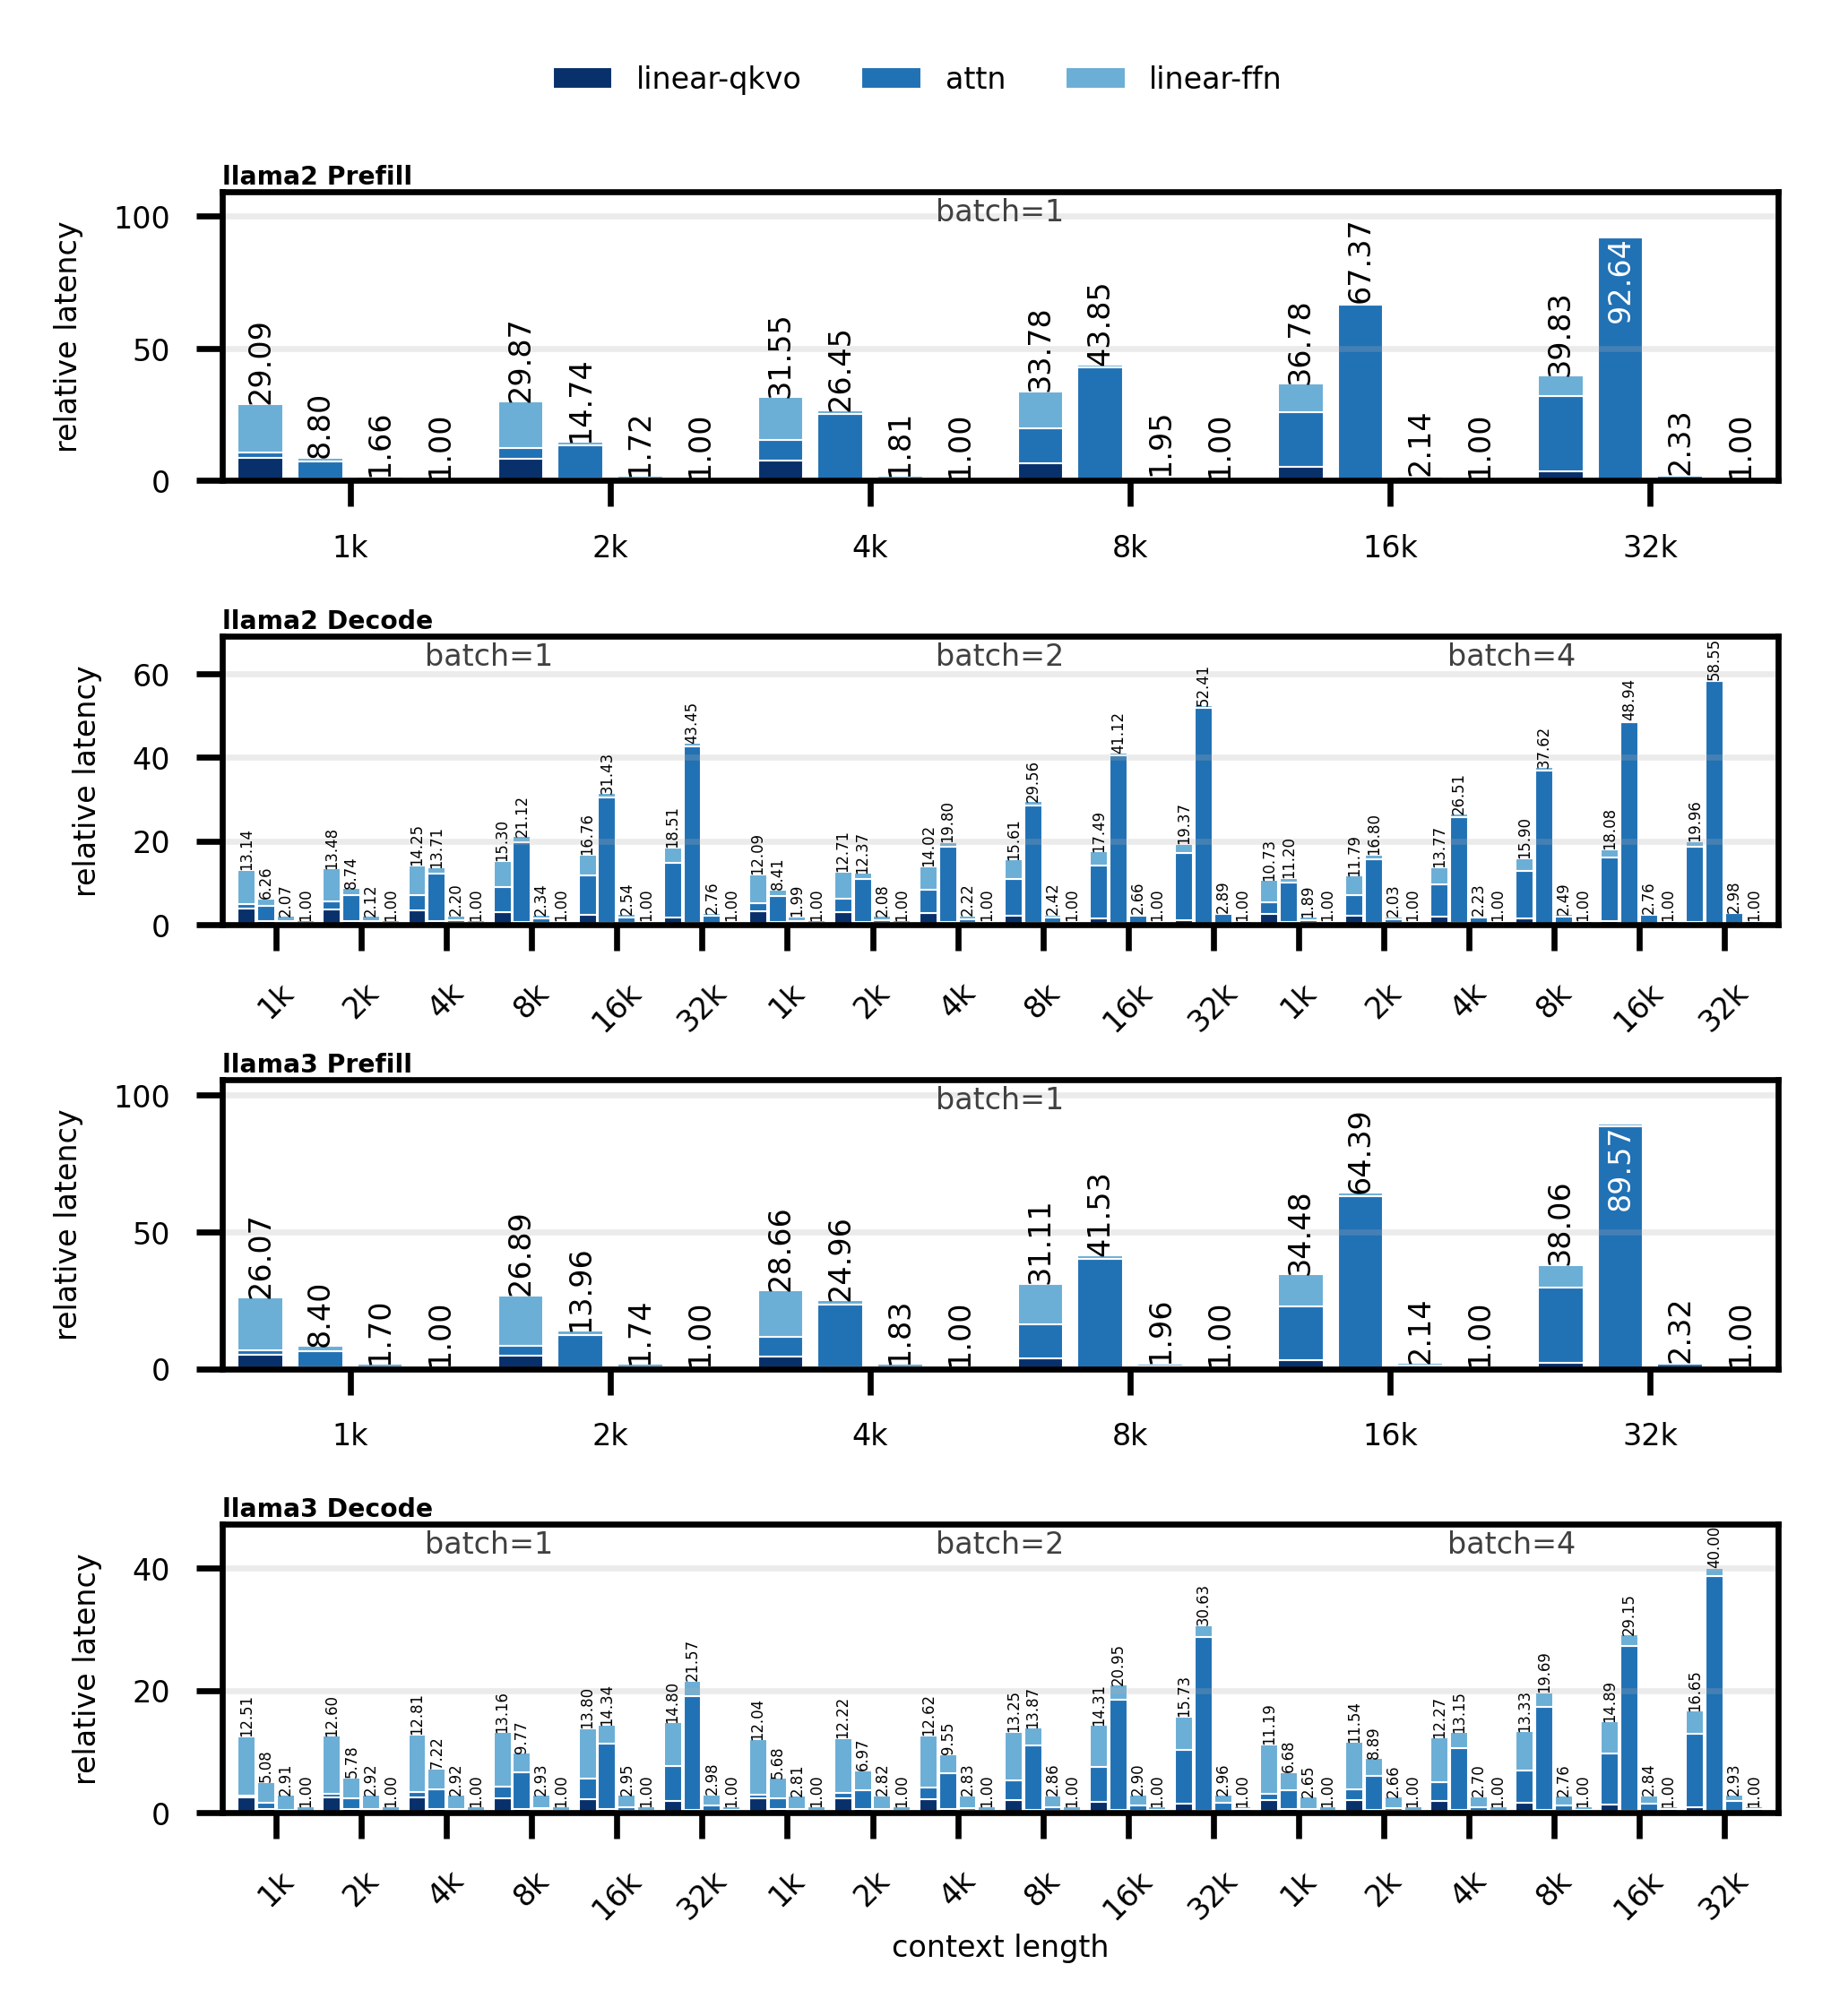
\includegraphics[width=\columnwidth]{figures/llama2_3/figures_script/llama_gemm_only/llama_gemm_only_latency.png}
    \caption{Area-normalized GEMM latency breakdown for linear projections and attention. Within each workload, the four stacked bars from left to right represent C1--C4 and are normalized to C4. Colors group the Q/K/V/O projections, attention GEMMs, and FFN projections.}
    \label{fig:gemm-breakdown}
\end{figure}

\subsection{End-to-End Energy Efficiency}

\begin{figure}[t]
    \centering
    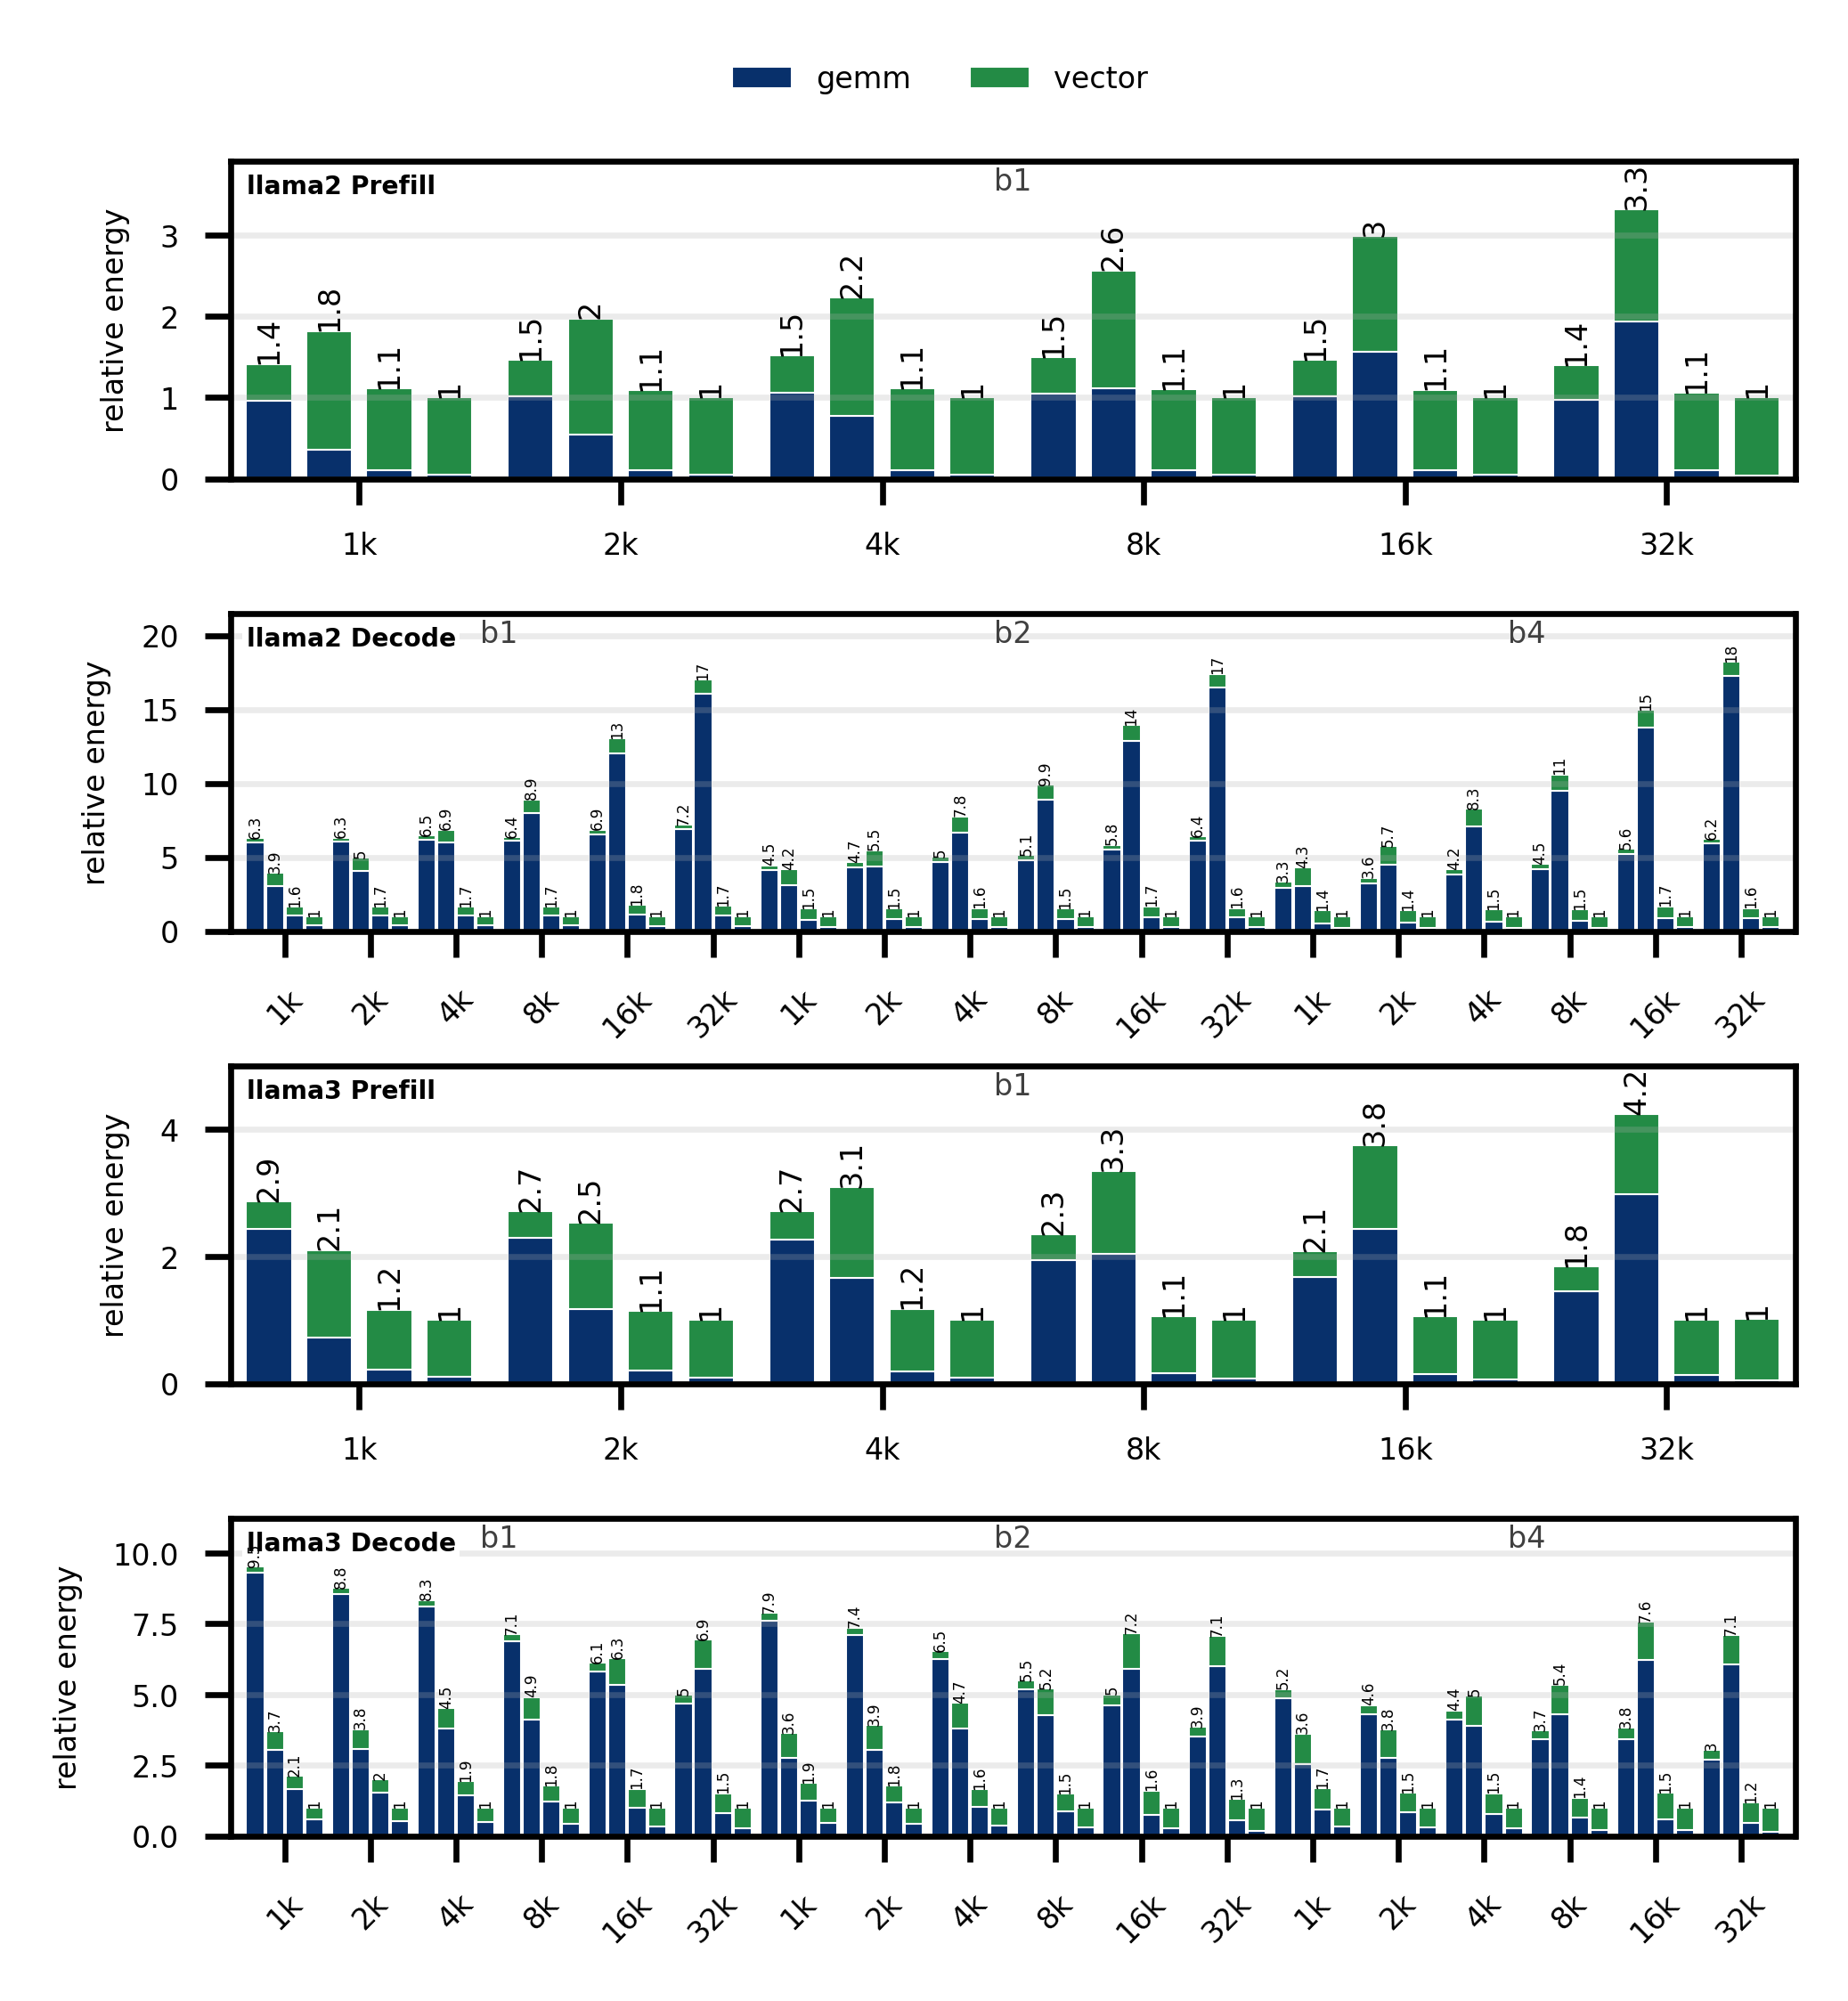
\includegraphics[width=\columnwidth]{figures/llama2_3/figures_script/llama_energy_stacked/llama_energy_per_token_power_dynamic_avg_W_stacked.png}
    \caption{End-to-end energy per token with idle power subtracted. Within each workload, the four bars from left to right represent C1--C4 and are normalized to C4. The vector portion includes all non-GEMM kernels, including fused layout transformations.}
    \label{fig:energy_per_token}
\end{figure}

Figure~\ref{fig:energy_per_token} reports end-to-end energy per token after subtracting idle board power. 
\Cfou{} reduces energy per token over C1 by $4.75\times$ on geomean in prefill and $7.93\times$ on geomean in decode.
The energy results broadly follow the latency trend.

C2 provides only a mixed energy benefit, reducing geomean energy over C1 by $1.07\times$ in prefill, whereas its decode energy is $1.19\times$ that of C1.
C3 reduces energy over C2 by $3.13\times$ in prefill and $3.46\times$ in decode, and C4 further reduces it over C3 by $1.42\times$ and $2.72\times$, respectively.
Thus, the same progression from native \fpint{} attention to the optimized memory and runtime system improves both latency and energy.

At the component level, C4 reduces GEMM energy over C1 by $37.24\times$ in prefill and $20.79\times$ in decode.
After this reduction, vector kernels account for an average of 88.4\% of C4's remaining energy in prefill and 61.4\% in decode.
The energy bottleneck therefore shifts toward vector processing, particularly during prefill.
\end{comment}

\subsection{Accuracy}

\begin{table*}[t]
\centering
\caption{Zero-shot accuracy (\%) on eight downstream tasks and WikiText-2 perplexity (PPL) for Llama2-7B W4A16KV4 variants.}
\label{tab:accuracy}

\scriptsize
\setlength{\tabcolsep}{1.5pt}
\begin{tabularx}{\textwidth}{@{}>{\raggedright\arraybackslash}p{0.18\textwidth}YYYYYYYYY|Y@{}}
\toprule
& ARC-c & ARC-e & BoolQ & HellaSwag & OBQA & PIQA & SocialQA & WinoG & Avg. $\uparrow$ & PPL $\downarrow$ \\
\midrule
W4A16KV4 & 44.20 & 73.15 & 76.85 & 75.35 & 42.60 & 78.56 & 45.24 & 68.82 & 63.10 & 5.59 \\
W4A16KV4 (linear) & 44.37 & 72.98 & 76.24 & 75.34 & 43.20 & 78.40 & 45.29 & 69.22 & 63.13 & 5.59 \\
W4A16KV4 (attn) & 44.03 & 73.32 & 76.82 & 75.23 & 43.20 & 78.56 & 44.73 & 68.19 & 63.01 & 5.59 \\
\rowcolor{gray!12}
W4A16KV4 (linear and attn)
& 44.03 & 73.02 & 77.13 & 75.22 & 44.20 & 78.78 & 45.24 & 69.53 & 63.39 & 5.59\\
\bottomrule
\end{tabularx}
\end{table*}

This experiment evaluates whether executing an already quantized model on the native \fpint{} datapath changes its accuracy relative to GPU execution.
Table~\ref{tab:accuracy} compares Llama2-7B with SpinQuant W4A16KV4 using the GPU reference and native \fpint{} execution for linear layers, attention, or both.
Across the eight zero-shot tasks, the GPU reference and the proposed hardware achieve average accuracies of 63.10 and 63.39, respectively, a difference of only 0.29 percentage points; both also achieve the same WikiText-2 perplexity of 5.59.
The intermediate configurations remain within the same narrow range, showing that executing both linear layers and attention on the proposed hardware introduces no measurable accuracy degradation at the reported precision.

\subsection{Hardware Efficiency and Area Overhead}

\paragraph{Array-level efficiency and attention-support overhead}
Table~\ref{tab:array-level} shows that the WKV \fpint{} GEMM engine improves TOPS/mm$^2$ by $2.21\times$ and TOPS/W by $2.97\times$ over the FP TCU.
Compared with the weight-only GEMM engine, supporting native KV-attention GEMMs reduces these efficiencies by only 4.4\% and 2.6\%, respectively.
As shown in Figure~\ref{fig:arr-level-break}, the additional \qrow{} input scaler accounts for only 3.41\% of the WKV GEMM engine area and 0.60\% of its power.
This low overhead results from sharing 32 FP multipliers across the GEMM engine columns instead of placing 1024 multipliers across the PEs.

\begin{table}[t]
\centering
\caption{Array-level efficiency at 28\,nm and 100\,MHz for a 32$\times$32 array, normalized to the FP TCU.}
\label{tab:array-level}
\small
\setlength{\tabcolsep}{3pt}
\begin{tabularx}{\columnwidth}{@{}>{\raggedright\arraybackslash}Xccc@{}}
\toprule
Unit & Precision & TOPS/mm$^2$ & TOPS/W \\
\midrule
FP TCU & FP$\times$FP & 1.0 & 1.0 \\
WoQ \fpint{} GEMM Engine & \fpint{} & 2.32 & 3.04 \\
WKV \fpint{} GEMM Engine & \fpint{} & 2.21 & 2.97 \\
\bottomrule
\end{tabularx}
\end{table}

\begin{figure}[t]
    \centering
    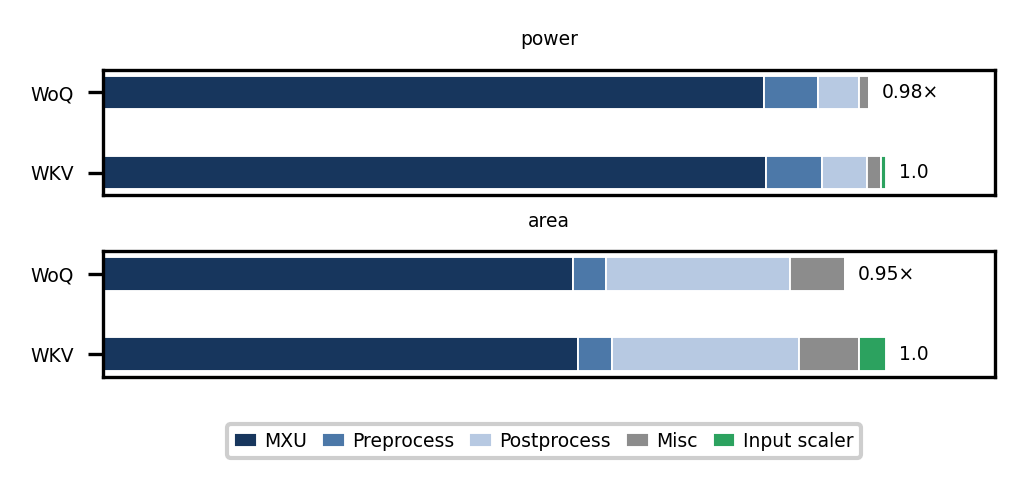
\includegraphics[width=\linewidth]{figures/gemm_engine_breakdown/fig10_wkv_vs_woq_relative_breakdown.png}
    \caption{Power and area breakdown of the weight-only (WoQ) and WKV \fpint{} GEMM engine.}
    \label{fig:arr-level-break}
\end{figure}

\paragraph{System-level area overhead}
Figure~\ref{fig:area-breakdown} shows that the GEMM engine and on-chip memories account for 43.6\% and 30.7\% of the total area, respectively, while the SIMT pipeline excluding memories accounts for 21.4\%.
In contrast, the DMA logic occupies 1.8\%, and miscellaneous logic including the interconnect and mux/demux occupies 2.6\%.
Their combined 4.3\% area overhead shows that the low-cost tensor path preserves the array-level density advantage at the full-system level.

\begin{figure}[t]
    \centering
    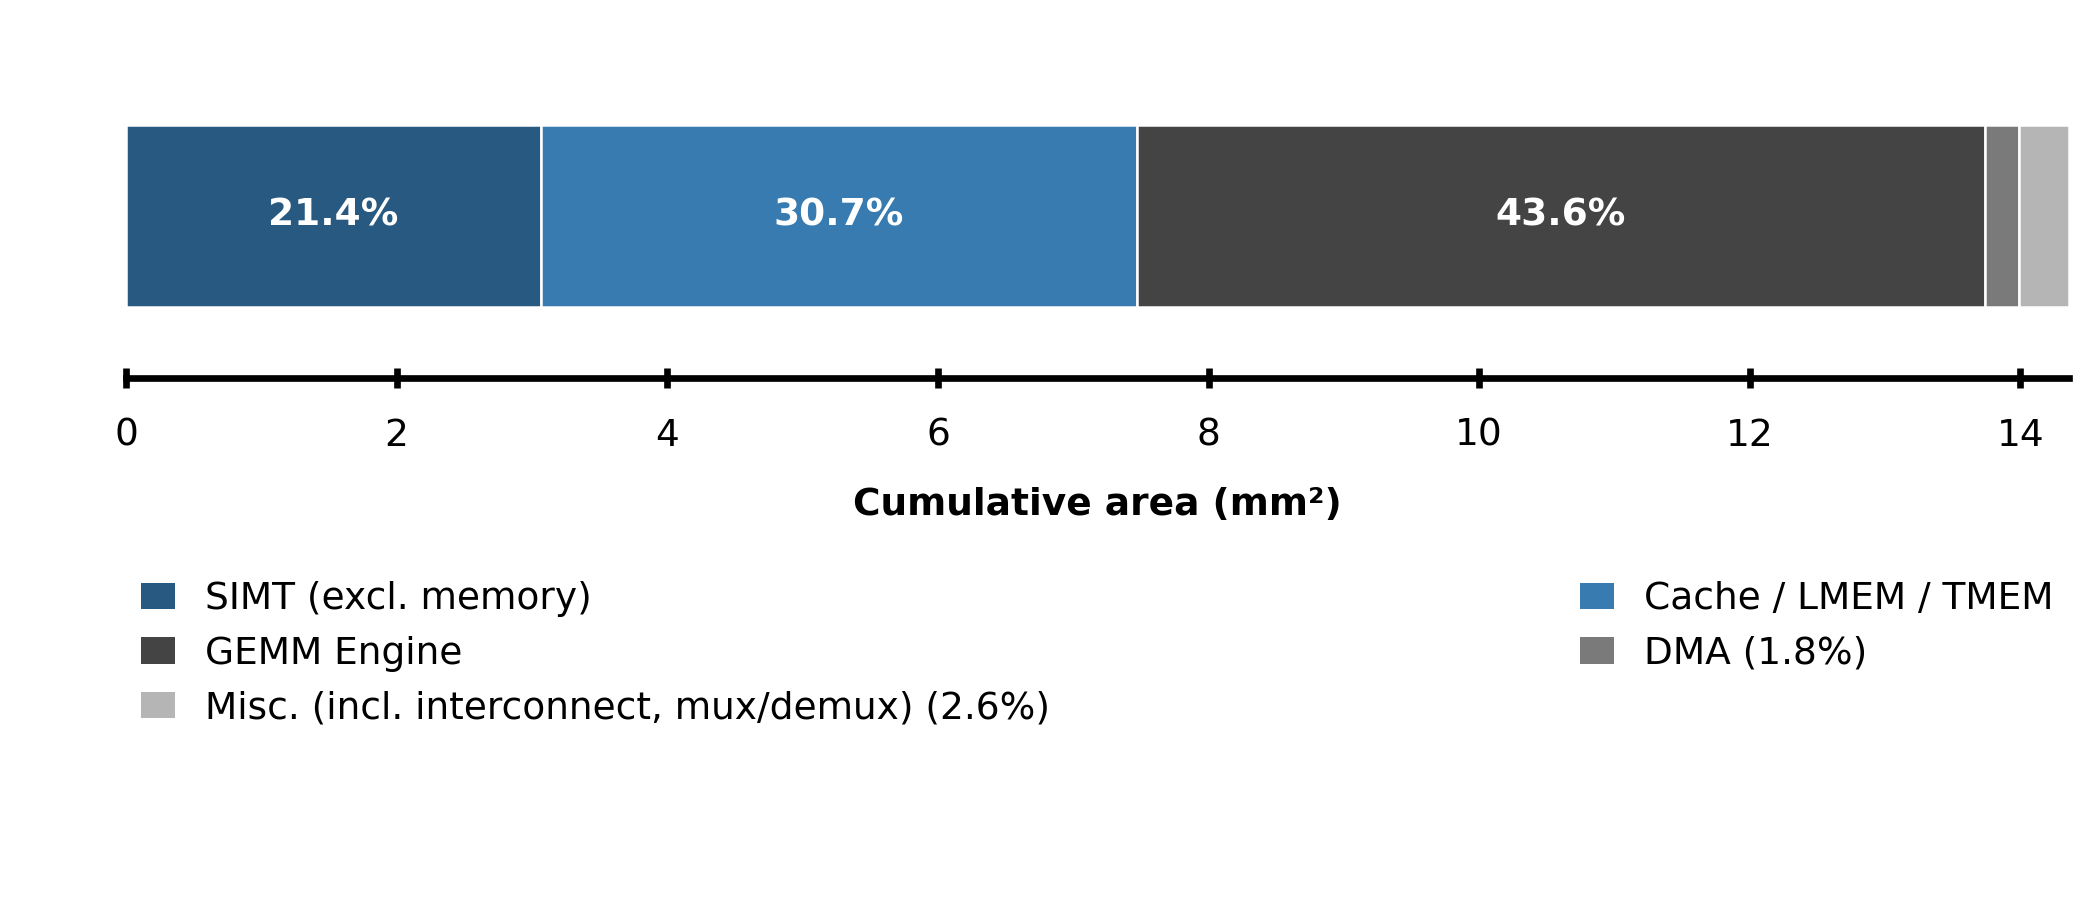
\includegraphics[width=\linewidth]{figures/top_breakdown/vortex_axi_breakdown.png}
    \caption{Full-system area breakdown of \ours{}, showing that the restricted tensor path keeps DMA and interconnect overhead low.}
    \label{fig:area-breakdown}
\end{figure}

\section{Conclusion}
WKV quantization turns both linear layers and KV-attention GEMMs into \fpint{} operations.
Realizing its benefit therefore requires native \fpint{} execution across the full model and a system that can efficiently feed the larger compute array.

\ours{} combines an \fpint{} GEMM engine with reconfigurable quantization and load directions, native $QK^T$ and PV kernels, decoupled GEMM execution, partitioned tensor and accumulator storage, and a dedicated cache-bypassed tensor path.
Tile-major layout, alignment-aware allocation, fused layout transformations, and explicit synchronization and cache management allow the runtime and kernels to satisfy the constraints of the simplified memory interconnect.

At the array level, the WKV \fpint{} GEMM engine improves TOPS/mm$^2$ by $2.21\times$ and TOPS/W by $2.97\times$ over the FP TCU, while DMA and miscellaneous interconnect logic account for only 3.5\% of the full-system area.
Across Llama2-7B and Llama3-8B W4A16KV4 inference, \ours{} reduces area-normalized end-to-end latency over the FP TCU baseline by $3.24\times$ on geomean in prefill and $4.73\times$ on geomean in decode, while reducing energy per token by $4.75\times$ and $7.93\times$, respectively.
For Llama2-7B, native \fpint{} execution introduces no measurable accuracy degradation relative to GPU execution.
These results demonstrate that array-level \fpint{} efficiency can be translated into system-level LLM inference improvements through full-stack co-design.

%%%%%%% -- PAPER CONTENT ENDS -- %%%%%%%%


%%%%%%%%% -- BIB STYLE AND FILE -- %%%%%%%%
\bibliographystyle{IEEEtranS}
\bibliography{refs}
%%%%%%%%%%%%%%%%%%%%%%%%%%%%%%%%%%%%

% \begin{figure}[t]
%     \centering
%     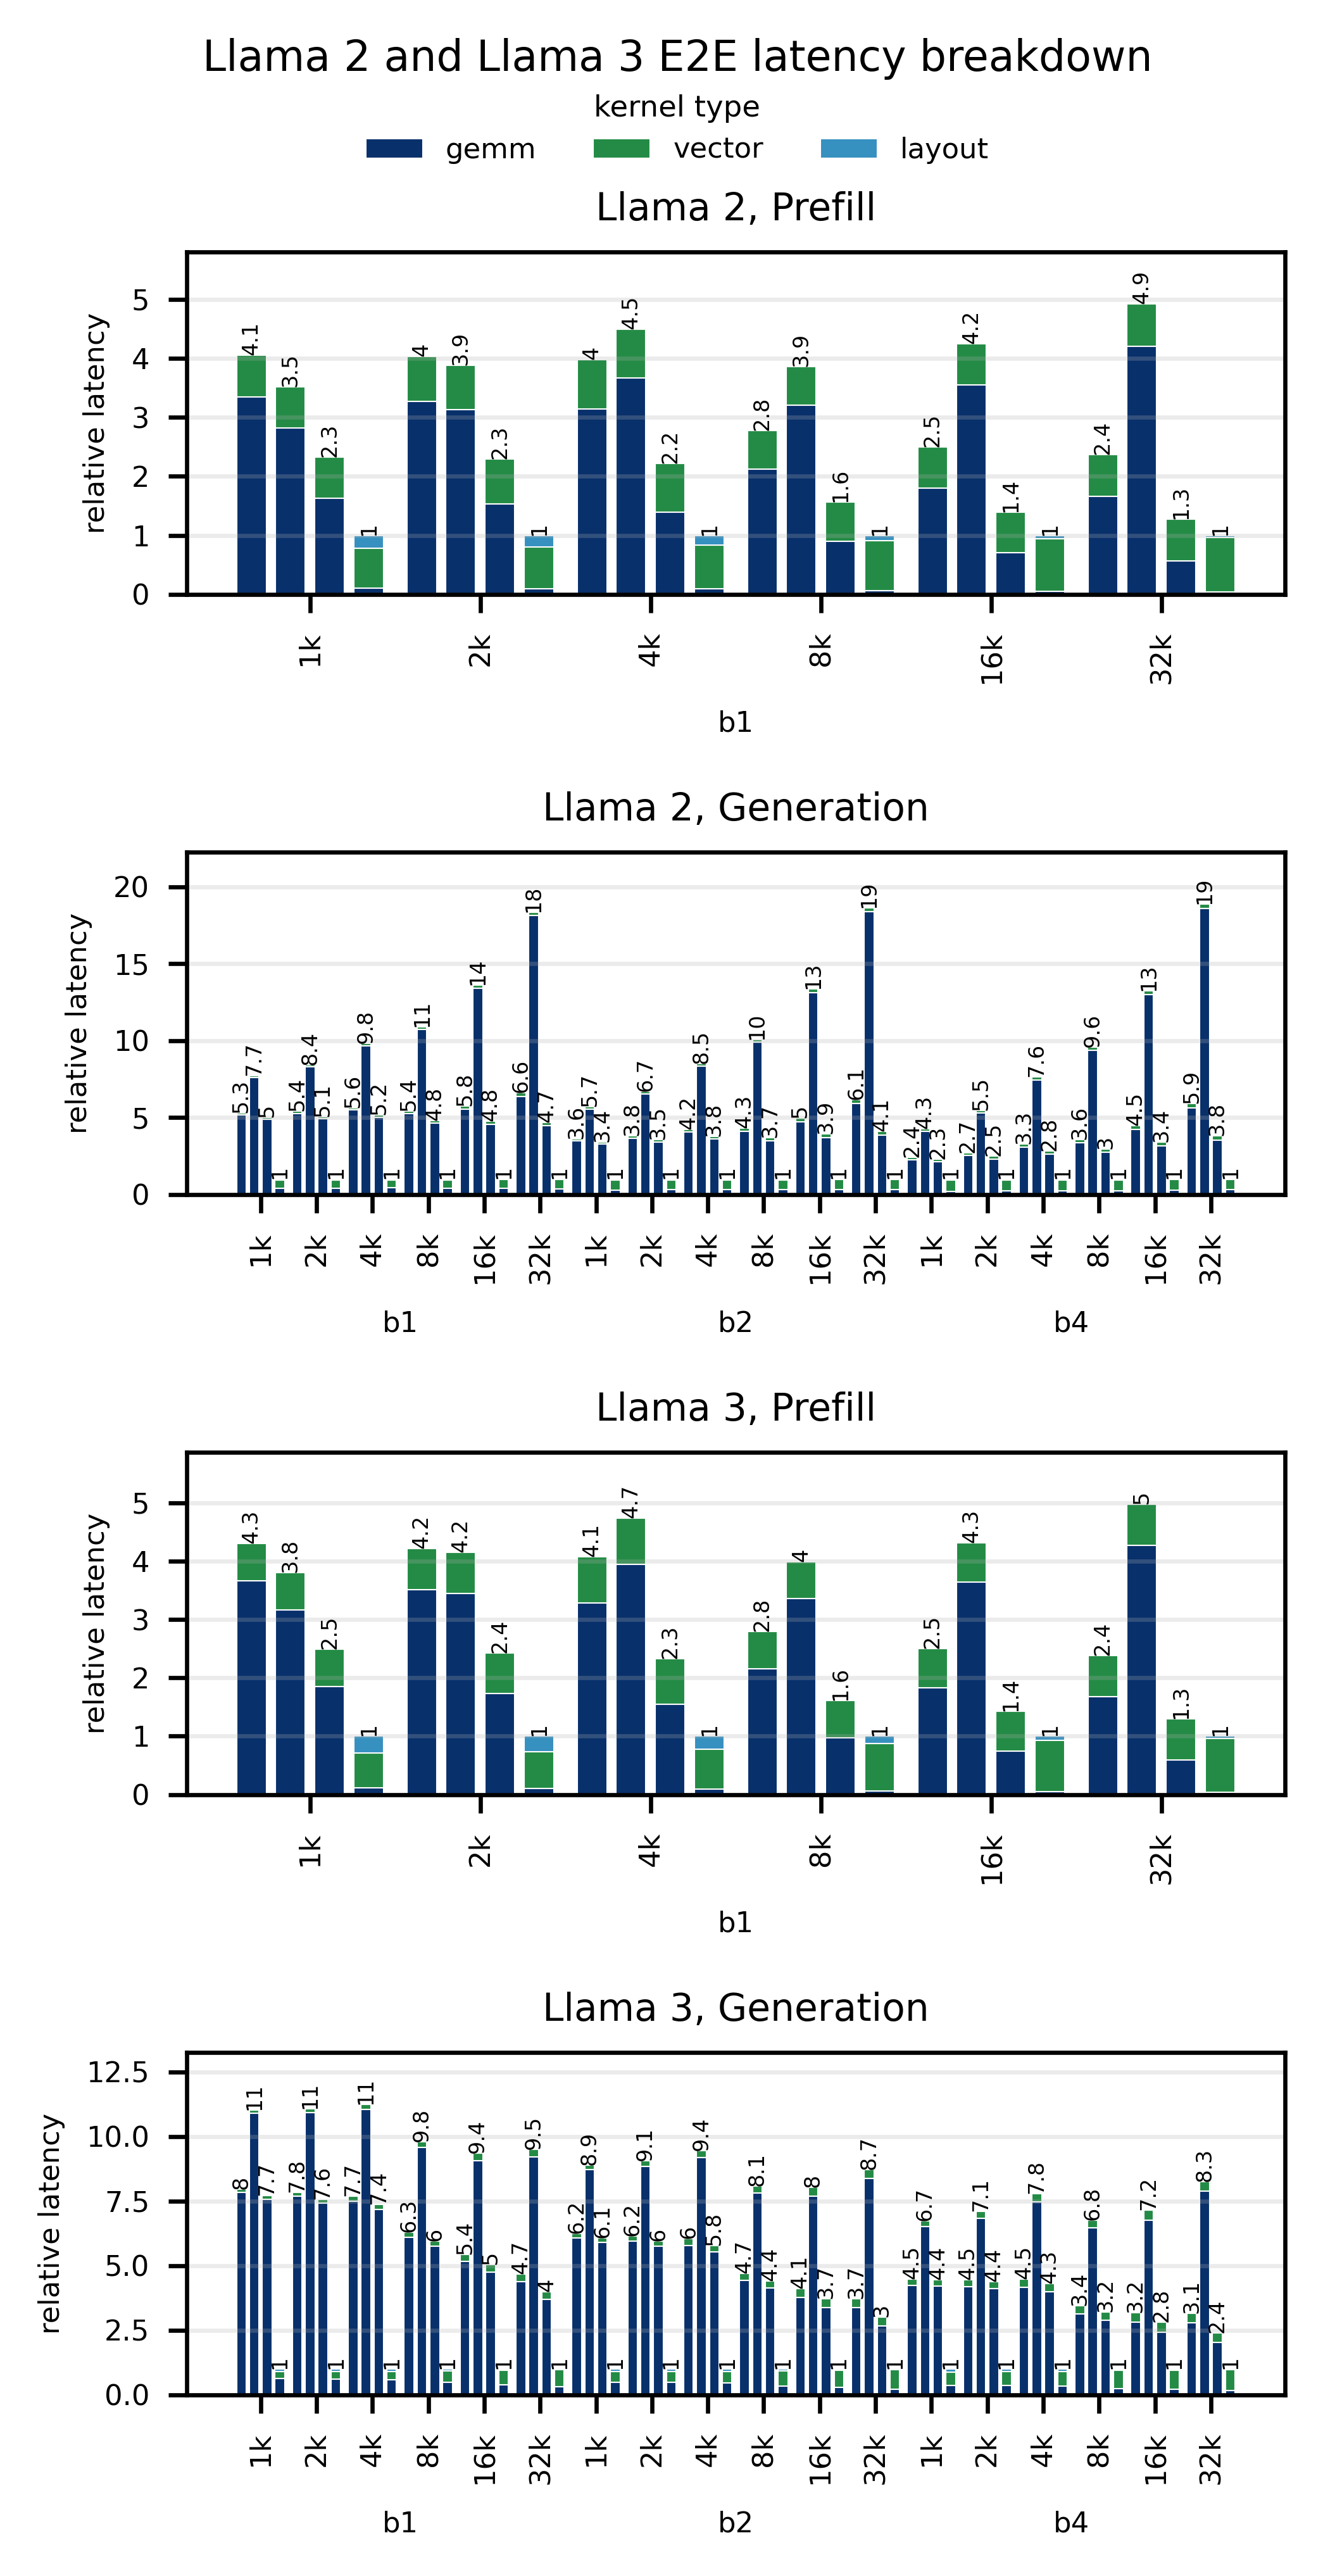
\includegraphics[width=\columnwidth]{figures/llama_e2e_latency_stacked.png}
%     \caption{one column test}
%     \label{fig:one-col-test}
% \end{figure}

\end{document}
